\chapter{Desarrollo de la interfaz de usuario}
En Ingeniería del Software nos enseñaron que para añadir una interfaz de usuario a un sistema ya hecho no había que modificar el sistema ya existente. Hay metodologías que empiezan haciendo una interfaz de usuario ``vacía'' y, a partir de ahí, van añadiéndole funcionalidad a sus botones. En nuestro caso hemos optado por el primer principio, ya que nos pareció la forma más natural de hacerlo. A continuación, explicaré cómo hice para conectar la aplicación web que he desarrollado como interfaz de usuario con el programa \texttt{Python} que calcula el horario.

\section{Diseño de la interfaz}
Antes de empezar a programar, estuve pensando cómo debería ser la interfaz. Mi objetivo era hacerla lo más sencilla posible. Lo ideal hubiese sido que el programa funcionase simplemente con pulsar un botón, pero por desgracia tuve que ponerle algunas cosas más debido a su complejidad.

En primer lugar, diseñé una primera pantalla de bienvenida en la que se le solicititaban al usuario los datos necesarios para hacer el horario: días, horas y cuatrimestre. No quise añadir nada más a esta pantalla para hacerlo lo más sencillo posible. En la \hyperref[init]{Figura \ref*{init}} se puede ver un esquema sencillo de esta idea. Es un simple formulario con tres campos y un botón para subir dichos datos al servidor. ¿Para qué más?

\begin{figure}
\centering
\scalebox{.7}{% Graphic for TeX using PGF
% Title: /home/marta/Diagrama1.dia
% Creator: Dia v0.97.3
% CreationDate: Fri Sep  8 23:31:58 2017
% For: marta
% \usepackage{tikz}
% The following commands are not supported in PSTricks at present
% We define them conditionally, so when they are implemented,
% this pgf file will use them.
\ifx\du\undefined
  \newlength{\du}
\fi
\setlength{\du}{15\unitlength}
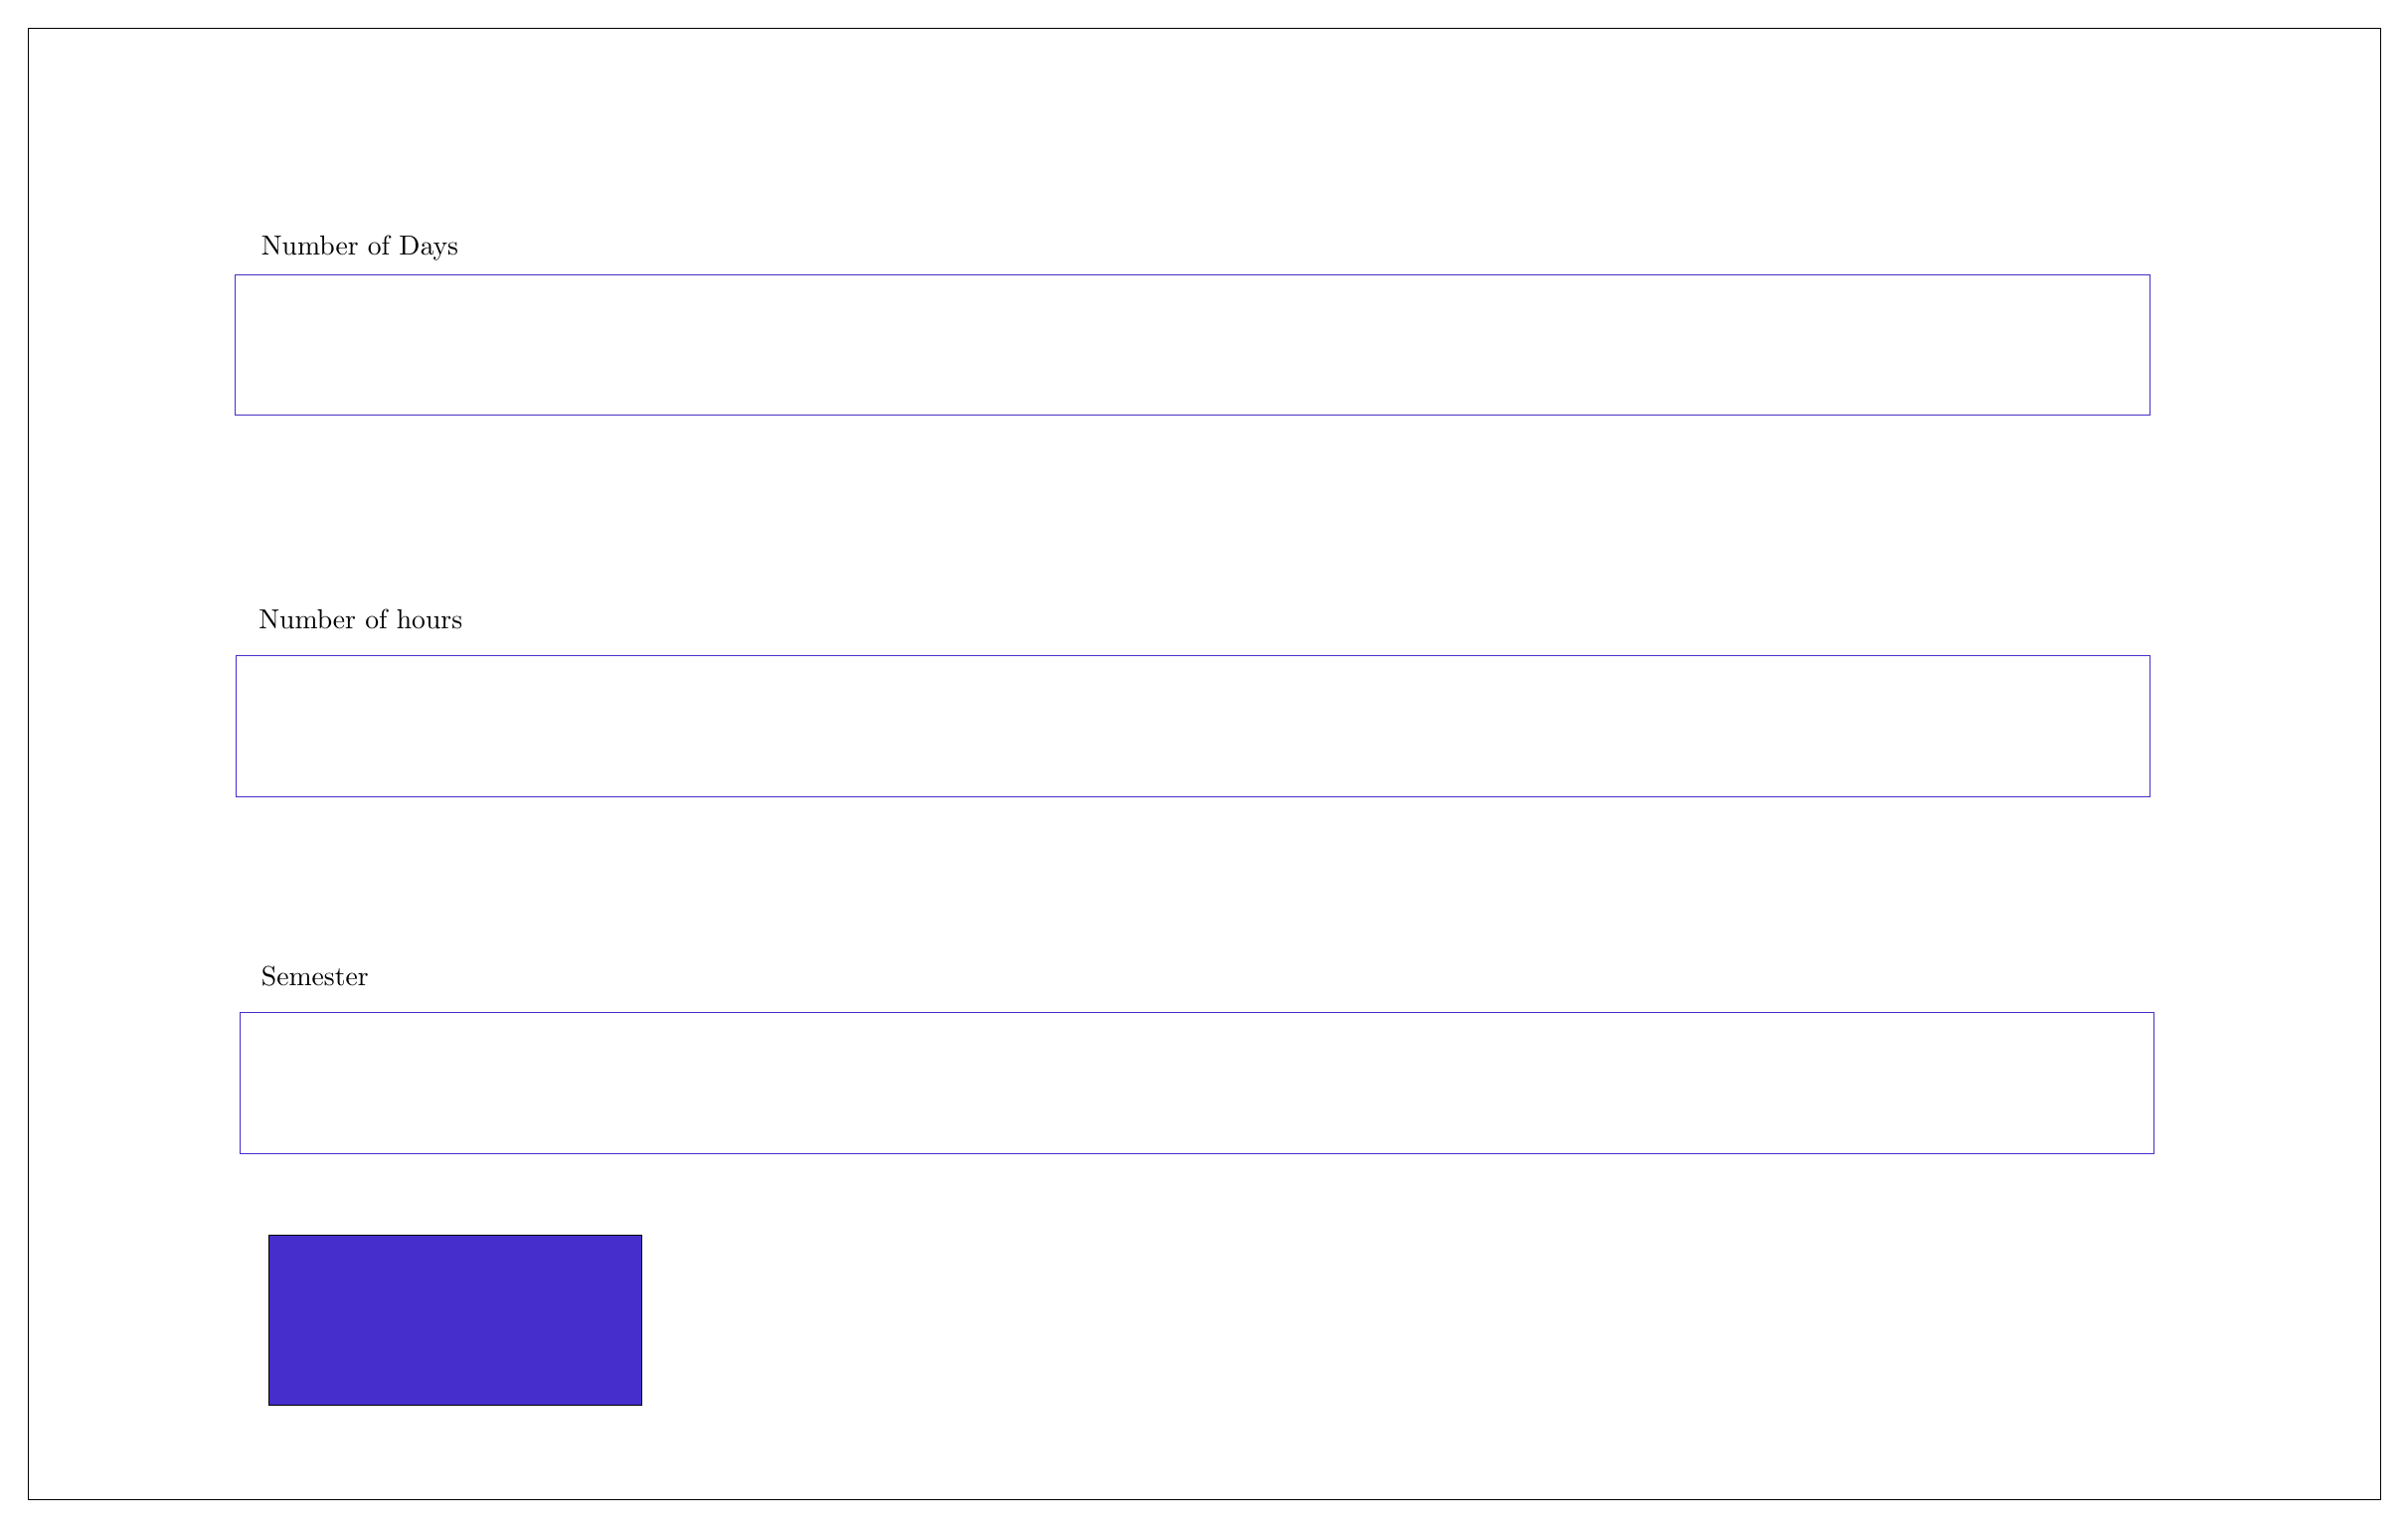
\begin{tikzpicture}
\pgftransformxscale{1.000000}
\pgftransformyscale{-1.000000}
\definecolor{dialinecolor}{rgb}{0.000000, 0.000000, 0.000000}
\pgfsetstrokecolor{dialinecolor}
\definecolor{dialinecolor}{rgb}{1.000000, 1.000000, 1.000000}
\pgfsetfillcolor{dialinecolor}
\pgfsetlinewidth{0.100000\du}
\pgfsetdash{}{0pt}
\pgfsetdash{}{0pt}
\pgfsetmiterjoin
\definecolor{dialinecolor}{rgb}{1.000000, 1.000000, 1.000000}
\pgfsetfillcolor{dialinecolor}
\fill (5.150000\du,4.950000\du)--(5.150000\du,23.750000\du)--(35.200000\du,23.750000\du)--(35.200000\du,4.950000\du)--cycle;
\definecolor{dialinecolor}{rgb}{0.000000, 0.000000, 0.000000}
\pgfsetstrokecolor{dialinecolor}
\draw (5.150000\du,4.950000\du)--(5.150000\du,23.750000\du)--(35.200000\du,23.750000\du)--(35.200000\du,4.950000\du)--cycle;
\pgfsetlinewidth{0.100000\du}
\pgfsetdash{}{0pt}
\pgfsetdash{}{0pt}
\pgfsetmiterjoin
\definecolor{dialinecolor}{rgb}{1.000000, 1.000000, 1.000000}
\pgfsetfillcolor{dialinecolor}
\fill (7.800000\du,8.100000\du)--(7.800000\du,9.900000\du)--(32.250000\du,9.900000\du)--(32.250000\du,8.100000\du)--cycle;
\definecolor{dialinecolor}{rgb}{0.270588, 0.180392, 0.800000}
\pgfsetstrokecolor{dialinecolor}
\draw (7.800000\du,8.100000\du)--(7.800000\du,9.900000\du)--(32.250000\du,9.900000\du)--(32.250000\du,8.100000\du)--cycle;
\pgfsetlinewidth{0.100000\du}
\pgfsetdash{}{0pt}
\pgfsetdash{}{0pt}
\pgfsetmiterjoin
\definecolor{dialinecolor}{rgb}{1.000000, 1.000000, 1.000000}
\pgfsetfillcolor{dialinecolor}
\fill (7.810375\du,12.965000\du)--(7.810375\du,14.765000\du)--(32.260375\du,14.765000\du)--(32.260375\du,12.965000\du)--cycle;
\definecolor{dialinecolor}{rgb}{0.270588, 0.180392, 0.800000}
\pgfsetstrokecolor{dialinecolor}
\draw (7.810375\du,12.965000\du)--(7.810375\du,14.765000\du)--(32.260375\du,14.765000\du)--(32.260375\du,12.965000\du)--cycle;
\pgfsetlinewidth{0.100000\du}
\pgfsetdash{}{0pt}
\pgfsetdash{}{0pt}
\pgfsetmiterjoin
\definecolor{dialinecolor}{rgb}{1.000000, 1.000000, 1.000000}
\pgfsetfillcolor{dialinecolor}
\fill (7.858300\du,17.530000\du)--(7.858300\du,19.330000\du)--(32.308300\du,19.330000\du)--(32.308300\du,17.530000\du)--cycle;
\definecolor{dialinecolor}{rgb}{0.270588, 0.180392, 0.800000}
\pgfsetstrokecolor{dialinecolor}
\draw (7.858300\du,17.530000\du)--(7.858300\du,19.330000\du)--(32.308300\du,19.330000\du)--(32.308300\du,17.530000\du)--cycle;
\pgfsetlinewidth{0.100000\du}
\pgfsetdash{}{0pt}
\pgfsetdash{}{0pt}
\pgfsetmiterjoin
\definecolor{dialinecolor}{rgb}{0.270588, 0.180392, 0.800000}
\pgfsetfillcolor{dialinecolor}
\fill (8.221807\du,20.371157\du)--(8.221807\du,22.543358\du)--(12.987683\du,22.543358\du)--(12.987683\du,20.371157\du)--cycle;
\definecolor{dialinecolor}{rgb}{0.000000, 0.000000, 0.000000}
\pgfsetstrokecolor{dialinecolor}
\draw (8.221807\du,20.371157\du)--(8.221807\du,22.543358\du)--(12.987683\du,22.543358\du)--(12.987683\du,20.371157\du)--cycle;
% setfont left to latex
\definecolor{dialinecolor}{rgb}{0.000000, 0.000000, 0.000000}
\pgfsetstrokecolor{dialinecolor}
\node[anchor=west] at (7.984733\du,12.502007\du){Number of hours};
% setfont left to latex
\definecolor{dialinecolor}{rgb}{0.000000, 0.000000, 0.000000}
\pgfsetstrokecolor{dialinecolor}
\node[anchor=west] at (8.017154\du,7.768553\du){Number of Days};
% setfont left to latex
\definecolor{dialinecolor}{rgb}{0.000000, 0.000000, 0.000000}
\pgfsetstrokecolor{dialinecolor}
\node[anchor=west] at (8.017154\du,17.073358\du){Semester};
\end{tikzpicture}
}
\caption{Pantalla inicial del programa}
\label{init}
\end{figure}

Después, diseñé la pantalla en la que se presentaría el horario final al usuario. En este caso, quise que el horario fuera lo más importante de la pantalla y el elemento que ocupase toda la atención. Para cambiar entre los horarios de cada grupo, decidí poner un menú \textit{dropdown}, pues era lo más disimulado. Me pareció que un sidebar ocupaba demasiado espacio y, un sidebar que se oculta y se muestra dinámicamente me pareció poco intuitivo. También añadí un botón para exportar el horario a PDF. En la \hyperref[horario]{Figura \ref*{horario}} se puede ver un esquema de esta pantalla.

\begin{figure}
\centering
\scalebox{.6}{% Graphic for TeX using PGF
% Title: /home/marta/Diagrama2.dia
% Creator: Dia v0.97.3
% CreationDate: Sat Sep  9 00:01:27 2017
% For: marta
% \usepackage{tikz}
% The following commands are not supported in PSTricks at present
% We define them conditionally, so when they are implemented,
% this pgf file will use them.
\ifx\du\undefined
  \newlength{\du}
\fi
\setlength{\du}{15\unitlength}
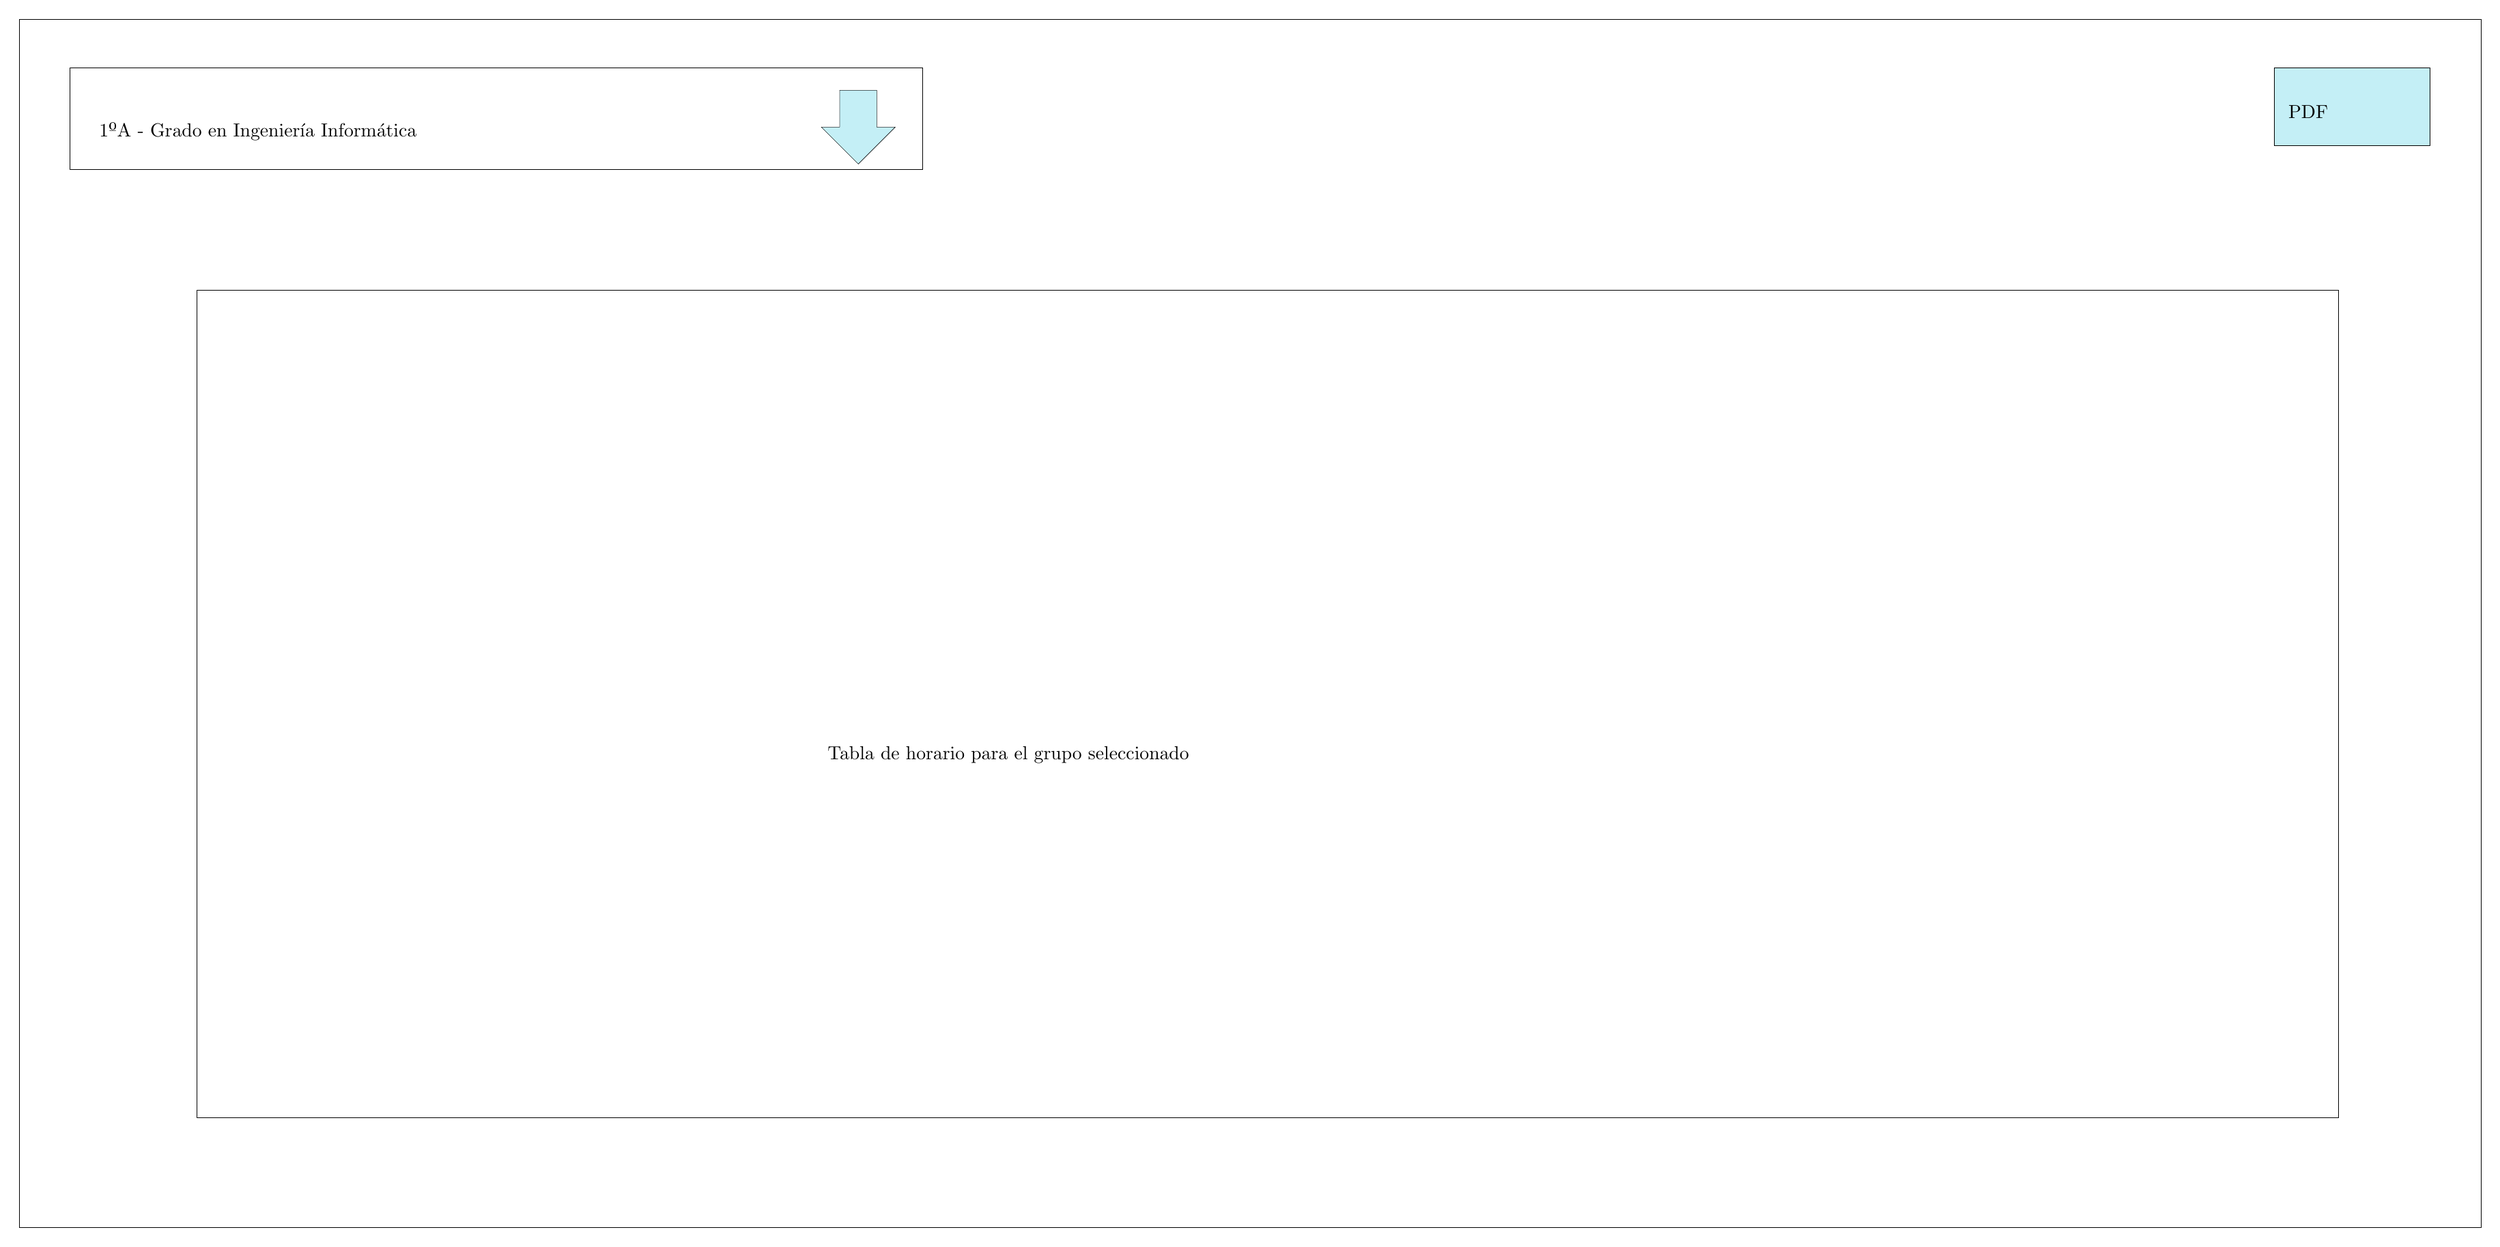
\begin{tikzpicture}
\pgftransformxscale{1.000000}
\pgftransformyscale{-1.000000}
\definecolor{dialinecolor}{rgb}{0.000000, 0.000000, 0.000000}
\pgfsetstrokecolor{dialinecolor}
\definecolor{dialinecolor}{rgb}{1.000000, 1.000000, 1.000000}
\pgfsetfillcolor{dialinecolor}
\pgfsetlinewidth{0.100000\du}
\pgfsetdash{}{0pt}
\pgfsetdash{}{0pt}
\pgfsetmiterjoin
\definecolor{dialinecolor}{rgb}{1.000000, 1.000000, 1.000000}
\pgfsetfillcolor{dialinecolor}
\fill (4.900000\du,2.550000\du)--(4.900000\du,25.050000\du)--(50.700000\du,25.050000\du)--(50.700000\du,2.550000\du)--cycle;
\definecolor{dialinecolor}{rgb}{0.000000, 0.000000, 0.000000}
\pgfsetstrokecolor{dialinecolor}
\draw (4.900000\du,2.550000\du)--(4.900000\du,25.050000\du)--(50.700000\du,25.050000\du)--(50.700000\du,2.550000\du)--cycle;
\pgfsetlinewidth{0.100000\du}
\pgfsetdash{}{0pt}
\pgfsetdash{}{0pt}
\pgfsetmiterjoin
\definecolor{dialinecolor}{rgb}{1.000000, 1.000000, 1.000000}
\pgfsetfillcolor{dialinecolor}
\fill (5.850000\du,3.450000\du)--(5.850000\du,5.350000\du)--(21.700000\du,5.350000\du)--(21.700000\du,3.450000\du)--cycle;
\definecolor{dialinecolor}{rgb}{0.000000, 0.000000, 0.000000}
\pgfsetstrokecolor{dialinecolor}
\draw (5.850000\du,3.450000\du)--(5.850000\du,5.350000\du)--(21.700000\du,5.350000\du)--(21.700000\du,3.450000\du)--cycle;
\pgfsetlinewidth{0.100000\du}
\pgfsetdash{}{0pt}
\pgfsetdash{}{0pt}
\pgfsetbuttcap
\pgfsetmiterjoin
\pgfsetlinewidth{0.100000\du}
\pgfsetbuttcap
\pgfsetmiterjoin
\pgfsetdash{}{0pt}
\definecolor{dialinecolor}{rgb}{0.768627, 0.937255, 0.964706}
\pgfsetfillcolor{dialinecolor}
\fill (20.168750\du,3.875000\du)--(20.168750\du,4.562500\du)--(19.825000\du,4.562500\du)--(20.512500\du,5.250000\du)--(21.200000\du,4.562500\du)--(20.856250\du,4.562500\du)--(20.856250\du,3.875000\du)--cycle;
\definecolor{dialinecolor}{rgb}{0.000000, 0.000000, 0.000000}
\pgfsetstrokecolor{dialinecolor}
\draw (20.168750\du,3.875000\du)--(20.168750\du,4.562500\du)--(19.825000\du,4.562500\du)--(20.512500\du,5.250000\du)--(21.200000\du,4.562500\du)--(20.856250\du,4.562500\du)--(20.856250\du,3.875000\du)--cycle;
\pgfsetbuttcap
\pgfsetmiterjoin
\pgfsetdash{}{0pt}
\definecolor{dialinecolor}{rgb}{0.000000, 0.000000, 0.000000}
\pgfsetstrokecolor{dialinecolor}
\draw (20.168750\du,3.875000\du)--(20.168750\du,4.562500\du)--(19.825000\du,4.562500\du)--(20.512500\du,5.250000\du)--(21.200000\du,4.562500\du)--(20.856250\du,4.562500\du)--(20.856250\du,3.875000\du)--cycle;
% setfont left to latex
\definecolor{dialinecolor}{rgb}{0.000000, 0.000000, 0.000000}
\pgfsetstrokecolor{dialinecolor}
\node[anchor=west] at (6.275000\du,4.650000\du){1ºA - Grado en Ingeniería Informática};
\pgfsetlinewidth{0.100000\du}
\pgfsetdash{}{0pt}
\pgfsetdash{}{0pt}
\pgfsetmiterjoin
\definecolor{dialinecolor}{rgb}{0.768627, 0.937255, 0.964706}
\pgfsetfillcolor{dialinecolor}
\fill (46.850000\du,3.450000\du)--(46.850000\du,4.900000\du)--(49.750000\du,4.900000\du)--(49.750000\du,3.450000\du)--cycle;
\definecolor{dialinecolor}{rgb}{0.000000, 0.000000, 0.000000}
\pgfsetstrokecolor{dialinecolor}
\draw (46.850000\du,3.450000\du)--(46.850000\du,4.900000\du)--(49.750000\du,4.900000\du)--(49.750000\du,3.450000\du)--cycle;
% setfont left to latex
\definecolor{dialinecolor}{rgb}{0.000000, 0.000000, 0.000000}
\pgfsetstrokecolor{dialinecolor}
\node[anchor=west] at (47.000000\du,4.275000\du){PDF};
\pgfsetlinewidth{0.100000\du}
\pgfsetdash{}{0pt}
\pgfsetdash{}{0pt}
\pgfsetmiterjoin
\definecolor{dialinecolor}{rgb}{1.000000, 1.000000, 1.000000}
\pgfsetfillcolor{dialinecolor}
\fill (8.200000\du,7.600000\du)--(8.200000\du,23.000000\du)--(48.050000\du,23.000000\du)--(48.050000\du,7.600000\du)--cycle;
\definecolor{dialinecolor}{rgb}{0.000000, 0.000000, 0.000000}
\pgfsetstrokecolor{dialinecolor}
\draw (8.200000\du,7.600000\du)--(8.200000\du,23.000000\du)--(48.050000\du,23.000000\du)--(48.050000\du,7.600000\du)--cycle;
% setfont left to latex
\definecolor{dialinecolor}{rgb}{0.000000, 0.000000, 0.000000}
\pgfsetstrokecolor{dialinecolor}
\node[anchor=west] at (19.825000\du,16.250000\du){Tabla de horario para el grupo seleccionado};
\end{tikzpicture}
}
\caption{Pantalla para mostrar el horario en el programa}
\label{horario}
\end{figure}

\section{Herramienta usada}
Actualmente, hay un montón de tecnologías o herramientas para hacer todo tipo de interfaces de usuario. Me limité a buscar herramientas para \texttt{Python}, pues así podía integrar de forma muy sencilla todo el trabajo previo ya realizado en este lenguaje. Si hubiese usado otras herramientas, tendría que haber un puente para intercambiar información entre ambas, lo que podría suponer un cuello de botella. Por ejemplo, para conectar Python con un servidor NodeJS, se tienen que hacer JSON que reciben como parámetro y devuelven ambas partes para intercambiar información. Hay herramientas en el mercado que están así implementadas, como por ejemplo, la Restful API de Wazuh (\url{https://github.com/wazuh/wazuh-api}). 

A la hora de hacer una interfaz de usuario en \textit{Python} tenía dos opciones: o bien hacer una interfaz usando \texttt{PyQt} (\url{https://wiki.python.org/moin/PyQt}) o bien hacer una \textit{aplicación web}. Finalmente, me decanté por hacer una aplicación web por las varias razones. En primer lugar, una aplicación web \textit{responsive} puede usarse tanto desde un teléfono móvil como desde un ordenador. Además, el uso de una aplicación web permite que varias personas trabajen a la vez sobre la misma usando una base de datos centralizada, en lugar de tener una copia de los datos en cada ordenador. Otra ventaja de hacer una aplicación web es que el programador se puede abstraer del sistema operativo, ya que se ejecutará en un navegador. Así, en lugar de hacer una aplicación para cada sistema operativo, sólo se hace una que se dejará ejecutando en un servidor y a la que los usuarios accederán desde su PC. Lo único que debe preocupar al programador es el navegador que se use, sobre todo si algún usuario aún sigue usando \textit{Internet Explorer}.

Cuando ya decidí qué tipo de interfaz de usuario haría, pasé a pensar con qué \textbf{herramienta} iba a hacerla. Estuve pensando en \texttt{Flask} (\url{http://flask.pocoo.org/}), pero finalmente lo descarté porque es un \textit{framework} que se usa (o se debería de usar) para hacer aplicaciones sencillas. De hecho, su eslogan es \textit{A Python Microframework}. A parte de esto, su documentación es un poco pobre. También estuve pensando en \texttt{Django} (\url{https://www.djangoproject.com/}). \texttt{Django} es fácilmente escalable, con sólo cambiar una línea en un fichero de configuración y hacer algún que otro pequeño ajuste más podemos pasar de usar \texttt{SQLite3} a usar \texttt{PostgreeSQL}, es decir, podemos pasar de usar un gestor de base de datos de ``juguete'' a uno muy potente. Además, tiene una documentación buenísima que incluye un montón de ejemplos ya hechos, además de un montón de explicaciones con muchísimo detalle. Y no solo eso, tiene además una comunidad enorme detrás, por lo que cualquier problema que surja estará resuelto en internet con bastante probabilidad.

\begin{figure}
\centering
\includegraphics[width=0.7\textwidth]{img/django_flask_trends}
\caption{Interés sobre \texttt{Django} (en azul) y sobre \texttt{Flask} a lo largo del último año en todo el mundo. Datos: Google Trends (\url{https://g.co/trends/CgxUq})}
\label{djangoflasktrends}
\end{figure}

De hecho, si consultamos los datos ofrecidos por \textit{Google Trends} (\hyperref[djangoflasktrends]{Figura \ref*{djangoflasktrends}}) podemos ver que \texttt{Django} es mucho más popular que \texttt{Flask}. Esta es una razón más para elegir uno sobre el otro. ¿Por qué? Porque si un \textit{framework} es popular, significa que tendrá una comunidad que lo mantendrá y dará soporte durante mucho más tiempo. 

\subsection{Django}
\subsubsection{Instalación}
Para instalar \texttt{Django}, lo único que tenemos que hacer es ejecutar el siguiente comando:

\begin{minted}{shell-session}
$ sudo pip install django
\end{minted}

O, si sólo queremos instalar \texttt{Django} de forma local al proyecto y no en nuestro sistema, podemos crear un \texttt{\textit{virtualenv}} (\url{https://virtualenv.pypa.io/en/stable/}). Con esto, evitamos tener nuestro sistema lleno de paquetes que sólo hemos usado para una cosa concreta. Además, también nos da más flexibilidad, pues nos permite tener instalada una versión concreta de un paquete y evita colisiones entre paquetes. 

Al igual que \texttt{Django}, \texttt{virtualenv} se instala desde \texttt{pip}:

\begin{minted}{shell-session}
$ sudo pip install virtualenv
[sudo] password for marta: 
Collecting virtualenv
  Downloading virtualenv-15.1.0-py2.py3-none-any.whl (1.8MB)
    100% |================================| 1.8MB 374kB/s 
Installing collected packages: virtualenv
Successfully installed virtualenv-15.1.0
\end{minted}

Una vez instalado, para crear un \texttt{virtualenv} en la carpeta de nuestro proyecto ejecutamos el siguiente comando:

\begin{minted}{shell-session}
$ virtualenv ENV
Using base prefix '/usr'
New python executable in ENV/bin/python
Installing setuptools, pip, wheel...done.
\end{minted}

Donde \texttt{ENV} es la carpeta en la que queremos crear el \texttt{virtualenv}. 

Una vez creado, veremos los siguientes directorios:

% \begin{minted}{shell-session}
% $ ls -l
% total 16
% drwxr-xr-x 2 marta marta 4096 sep  5 19:57 bin
% drwxr-xr-x 2 marta marta 4096 sep  5 19:57 include
% drwxr-xr-x 3 marta marta 4096 sep  5 19:57 lib
% -rw-r--r-- 1 marta marta   60 sep  5 19:57 pip-selfcheck.json
% \end{minted}

\begin{enumerate}[---]
\item Los directorios \texttt{lib} e \texttt{include} contienen librerías que instalamos en el \texttt{virtualenv}. Recién creado, sólo contienen el intérprete de \texttt{python}.
\item El directorio \texttt{bin} guarda los ejecutables tantp de los paquetes que instalaremos en el \texttt{virtualenv} como los ejecutables que necesita \texttt{virutalenv} para funcionar.
\end{enumerate}

Un \texttt{virtualenv} recién creado necesita ser activado. Para ello, ejecutamos:

\begin{minted}{shell-session}
$ source bin/activate
\end{minted}

Nada más ejecutarlo, se modificará el shell para indicarnos que estamos dentro del \texttt{virtualenv}. Si queremos ``salir'' del mismo, basta con ejecutar:

\begin{minted}{shell-session}
$ deactivate
\end{minted}

Y volveremos a nuestra shell normal.

Volviendo a la instalación de \texttt{Django}, ahora que tenemos nuestro \texttt{virtualenv} listo podemos instalar \texttt{Django} sin usar sudo:

\begin{minted}{shell-session}
$ pip install Django
Collecting Django
  Downloading Django-1.11.5-py2.py3-none-any.whl (6.9MB)
    100% |=================================| 7.0MB 152kB/s 
Collecting pytz (from Django)
  Downloading pytz-2017.2-py2.py3-none-any.whl (484kB)
    100% |=================================| 491kB 788kB/s 
Installing collected packages: pytz, Django
Successfully installed Django-1.11.5 pytz-2017.2
\end{minted}

Para comprobar que \texttt{Django} se ha instalado correctamente, usamos el siguiente comando:

\begin{minted}{shell-session}
$ python -m django --version
1.11.5
\end{minted}

\subsubsection{Creando un proyecto}
Una de las cosas que más me gusta de \texttt{Django}, es que él solo automatiza un montón de tareas. Así, como ellos mismos dicen en su documentación, el programador puede centrarse en programar única y exclusivamente. Con otros \textit{framework} tendría que estar todo un día preparando un entorno de desarrollo antes de poder ponerme manos a la obra, en cambio, lo único que tengo que hacer es ejecutar el siguiente comando:

\begin{minted}{shell-session}
$ django-admin startproject NOMBRE
\end{minted}

donde \texttt{NOMBRE} es el nombre que queremos darle a nuestro proyecto.

Este comando nos crea toda la estructura de directorios necesaria para empezar a trabajar. Dicha estructura es la que se ve en la \hyperref[djangoprojectfolders]{Figura \ref*{djangoprojectfolders}}.

\begin{figure}
\centering
\scalebox{.7}{% Graphic for TeX using PGF
% Title: /home/marta/Diagrama1.dia
% Creator: Dia v0.97.3
% CreationDate: Thu Sep  7 22:53:00 2017
% For: marta
% \usepackage{tikz}
% The following commands are not supported in PSTricks at present
% We define them conditionally, so when they are implemented,
% this pgf file will use them.
\ifx\du\undefined
  \newlength{\du}
\fi
\setlength{\du}{15\unitlength}
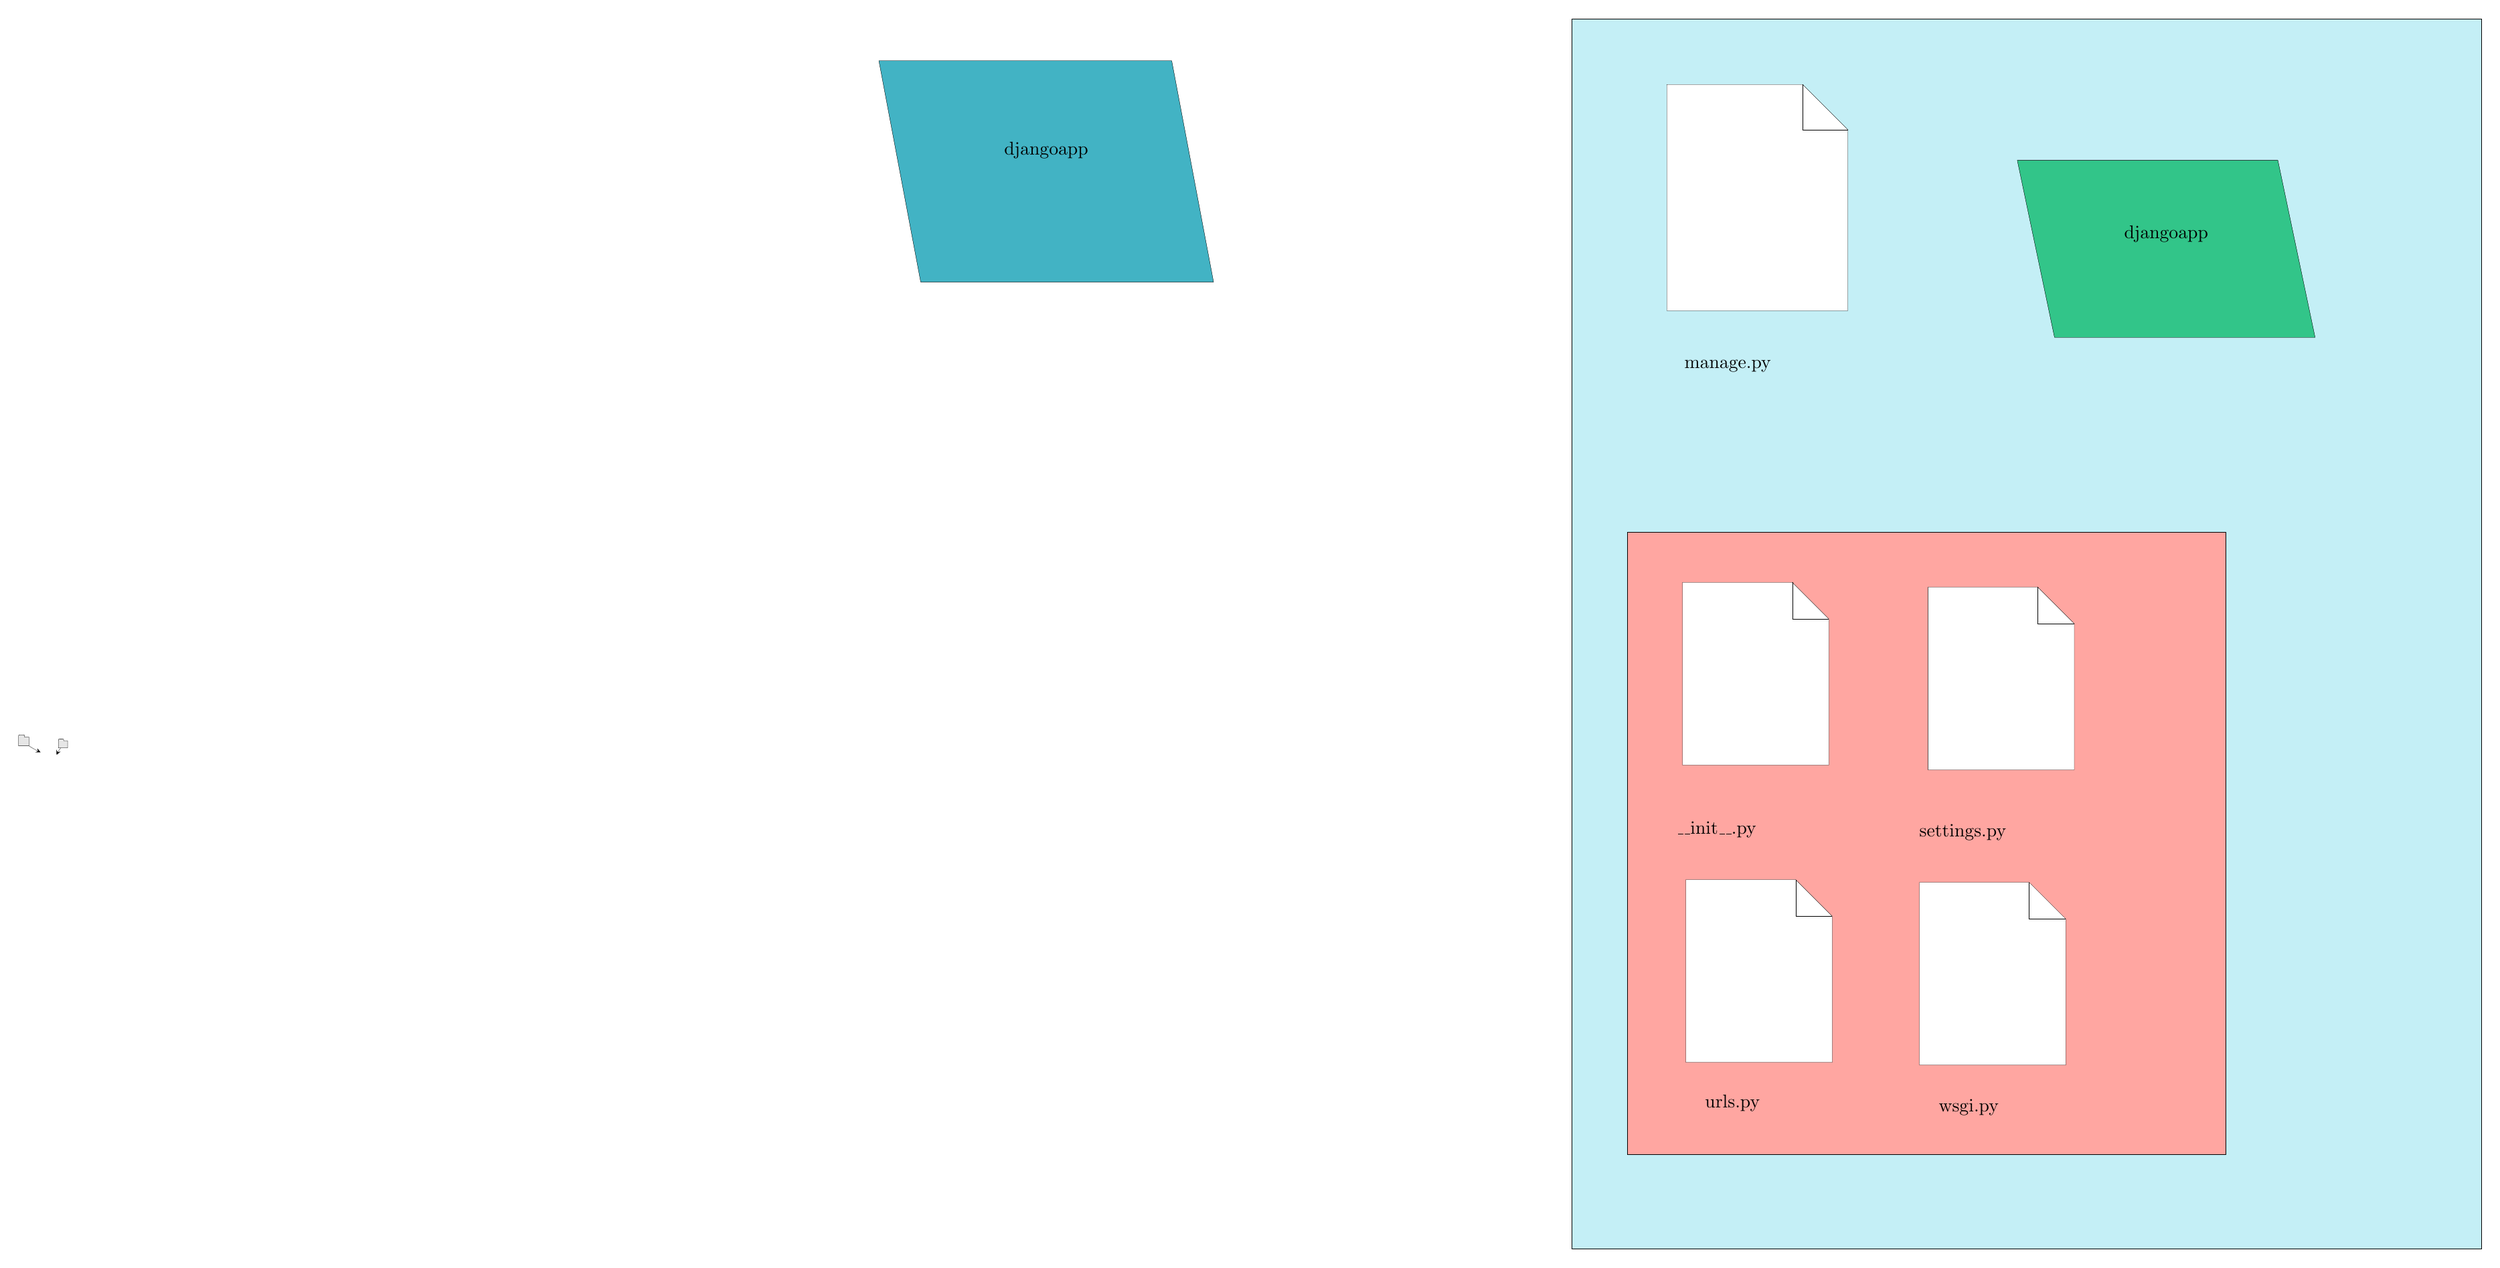
\begin{tikzpicture}
\pgftransformxscale{1.000000}
\pgftransformyscale{-1.000000}
\definecolor{dialinecolor}{rgb}{0.000000, 0.000000, 0.000000}
\pgfsetstrokecolor{dialinecolor}
\definecolor{dialinecolor}{rgb}{1.000000, 1.000000, 1.000000}
\pgfsetfillcolor{dialinecolor}
\pgfsetlinewidth{0.100000\du}
\pgfsetdash{}{0pt}
\pgfsetdash{}{0pt}
\pgfsetbuttcap
\pgfsetmiterjoin
\pgfsetlinewidth{0.100000\du}
\pgfsetbuttcap
\pgfsetmiterjoin
\pgfsetdash{}{0pt}
\definecolor{dialinecolor}{rgb}{0.901961, 0.901961, 0.901961}
\pgfsetfillcolor{dialinecolor}
\pgfpathmoveto{\pgfpoint{17.739413\du}{-13.924815\du}}
\pgfpathcurveto{\pgfpoint{17.739413\du}{-15.124814\du}}{\pgfpoint{17.739413\du}{-15.124814\du}}{\pgfpoint{18.533163\du}{-15.124814\du}}
\pgfpathcurveto{\pgfpoint{19.326913\du}{-15.124814\du}}{\pgfpoint{19.326913\du}{-15.124814\du}}{\pgfpoint{20.120663\du}{-15.124814\du}}
\pgfpathcurveto{\pgfpoint{20.914413\du}{-15.124814\du}}{\pgfpoint{20.914413\du}{-15.124814\du}}{\pgfpoint{20.914413\du}{-13.924815\du}}
\pgfpathcurveto{\pgfpoint{20.914413\du}{-13.924815\du}}{\pgfpoint{23.295663\du}{-13.924815\du}}{\pgfpoint{23.295663\du}{-13.924815\du}}
\pgfpathcurveto{\pgfpoint{23.295663\du}{-13.924815\du}}{\pgfpoint{23.295663\du}{-9.124814\du}}{\pgfpoint{23.295663\du}{-9.124814\du}}
\pgfpathcurveto{\pgfpoint{23.295663\du}{-9.124814\du}}{\pgfpoint{17.739413\du}{-9.124814\du}}{\pgfpoint{17.739413\du}{-9.124814\du}}
\pgfpathcurveto{\pgfpoint{17.739413\du}{-9.124814\du}}{\pgfpoint{17.739413\du}{-12.724814\du}}{\pgfpoint{17.739413\du}{-13.924815\du}}
\pgfusepath{fill}
\definecolor{dialinecolor}{rgb}{0.000000, 0.000000, 0.000000}
\pgfsetstrokecolor{dialinecolor}
\pgfpathmoveto{\pgfpoint{17.739413\du}{-13.924815\du}}
\pgfpathcurveto{\pgfpoint{17.739413\du}{-15.124814\du}}{\pgfpoint{17.739413\du}{-15.124814\du}}{\pgfpoint{18.533163\du}{-15.124814\du}}
\pgfpathcurveto{\pgfpoint{19.326913\du}{-15.124814\du}}{\pgfpoint{19.326913\du}{-15.124814\du}}{\pgfpoint{20.120663\du}{-15.124814\du}}
\pgfpathcurveto{\pgfpoint{20.914413\du}{-15.124814\du}}{\pgfpoint{20.914413\du}{-15.124814\du}}{\pgfpoint{20.914413\du}{-13.924815\du}}
\pgfpathcurveto{\pgfpoint{20.914413\du}{-13.924815\du}}{\pgfpoint{23.295663\du}{-13.924815\du}}{\pgfpoint{23.295663\du}{-13.924815\du}}
\pgfpathcurveto{\pgfpoint{23.295663\du}{-13.924815\du}}{\pgfpoint{23.295663\du}{-9.124814\du}}{\pgfpoint{23.295663\du}{-9.124814\du}}
\pgfpathcurveto{\pgfpoint{23.295663\du}{-9.124814\du}}{\pgfpoint{17.739413\du}{-9.124814\du}}{\pgfpoint{17.739413\du}{-9.124814\du}}
\pgfpathcurveto{\pgfpoint{17.739413\du}{-9.124814\du}}{\pgfpoint{17.739413\du}{-12.724814\du}}{\pgfpoint{17.739413\du}{-13.924815\du}}
\pgfusepath{stroke}
\pgfsetlinewidth{0.010000\du}
\pgfsetbuttcap
\pgfsetmiterjoin
\pgfsetdash{}{0pt}
\definecolor{dialinecolor}{rgb}{0.000000, 0.000000, 0.000000}
\pgfsetstrokecolor{dialinecolor}
\pgfpathmoveto{\pgfpoint{17.739413\du}{-13.924815\du}}
\pgfpathcurveto{\pgfpoint{17.739413\du}{-15.124814\du}}{\pgfpoint{17.739413\du}{-15.124814\du}}{\pgfpoint{18.533163\du}{-15.124814\du}}
\pgfpathcurveto{\pgfpoint{19.326913\du}{-15.124814\du}}{\pgfpoint{19.326913\du}{-15.124814\du}}{\pgfpoint{20.120663\du}{-15.124814\du}}
\pgfpathcurveto{\pgfpoint{20.914413\du}{-15.124814\du}}{\pgfpoint{20.914413\du}{-15.124814\du}}{\pgfpoint{20.914413\du}{-13.924815\du}}
\pgfpathcurveto{\pgfpoint{20.914413\du}{-13.924815\du}}{\pgfpoint{23.295663\du}{-13.924815\du}}{\pgfpoint{23.295663\du}{-13.924815\du}}
\pgfpathcurveto{\pgfpoint{23.295663\du}{-13.924815\du}}{\pgfpoint{23.295663\du}{-9.124814\du}}{\pgfpoint{23.295663\du}{-9.124814\du}}
\pgfpathcurveto{\pgfpoint{23.295663\du}{-9.124814\du}}{\pgfpoint{17.739413\du}{-9.124814\du}}{\pgfpoint{17.739413\du}{-9.124814\du}}
\pgfpathcurveto{\pgfpoint{17.739413\du}{-9.124814\du}}{\pgfpoint{17.739413\du}{-12.724814\du}}{\pgfpoint{17.739413\du}{-13.924815\du}}
\pgfusepath{stroke}
\pgfsetlinewidth{0.100000\du}
\pgfsetbuttcap
\pgfsetmiterjoin
\pgfsetdash{}{0pt}
\definecolor{dialinecolor}{rgb}{0.258824, 0.701961, 0.768627}
\pgfsetfillcolor{dialinecolor}
\fill (17.739413\du,-9.124814\du)--(16.945663\du,-13.324813\du)--(22.501913\du,-13.324813\du)--(23.295663\du,-9.124814\du)--cycle;
\definecolor{dialinecolor}{rgb}{0.000000, 0.000000, 0.000000}
\pgfsetstrokecolor{dialinecolor}
\draw (17.739413\du,-9.124814\du)--(16.945663\du,-13.324813\du)--(22.501913\du,-13.324813\du)--(23.295663\du,-9.124814\du)--cycle;
\pgfsetlinewidth{0.010000\du}
\pgfsetbuttcap
\pgfsetmiterjoin
\pgfsetdash{}{0pt}
\definecolor{dialinecolor}{rgb}{0.000000, 0.000000, 0.000000}
\pgfsetstrokecolor{dialinecolor}
\draw (17.739413\du,-9.124814\du)--(16.945663\du,-13.324813\du)--(22.501913\du,-13.324813\du)--(23.295663\du,-9.124814\du)--cycle;
% setfont left to latex
\definecolor{dialinecolor}{rgb}{1.000000, 1.000000, 1.000000}
\pgfsetstrokecolor{dialinecolor}
\node at (20.120663\du,-11.624814\du){djangoapp};
\pgfsetlinewidth{0.100000\du}
\pgfsetdash{}{0pt}
\pgfsetdash{}{0pt}
\pgfsetmiterjoin
\definecolor{dialinecolor}{rgb}{0.768627, 0.937255, 0.964706}
\pgfsetfillcolor{dialinecolor}
\fill (30.095663\du,-14.124814\du)--(30.095663\du,9.225186\du)--(47.345663\du,9.225186\du)--(47.345663\du,-14.124814\du)--cycle;
\definecolor{dialinecolor}{rgb}{0.000000, 0.000000, 0.000000}
\pgfsetstrokecolor{dialinecolor}
\draw (30.095663\du,-14.124814\du)--(30.095663\du,9.225186\du)--(47.345663\du,9.225186\du)--(47.345663\du,-14.124814\du)--cycle;
\pgfsetlinewidth{0.100000\du}
\pgfsetdash{}{0pt}
\pgfsetdash{}{0pt}
\pgfsetbuttcap
{
\definecolor{dialinecolor}{rgb}{0.000000, 0.000000, 0.000000}
\pgfsetfillcolor{dialinecolor}
% was here!!!
\pgfsetarrowsend{stealth}
\definecolor{dialinecolor}{rgb}{0.000000, 0.000000, 0.000000}
\pgfsetstrokecolor{dialinecolor}
\pgfpathmoveto{\pgfpoint{23.338714\du}{-9.126739\du}}
\pgfpatharc{123}{115}{51.064311\du and 51.064311\du}
\pgfusepath{stroke}
}
\pgfsetlinewidth{0.100000\du}
\pgfsetdash{}{0pt}
\pgfsetdash{}{0pt}
\pgfsetbuttcap
\pgfsetmiterjoin
\pgfsetlinewidth{0.100000\du}
\pgfsetbuttcap
\pgfsetmiterjoin
\pgfsetdash{}{0pt}
\definecolor{dialinecolor}{rgb}{1.000000, 1.000000, 1.000000}
\pgfsetfillcolor{dialinecolor}
\fill (31.895663\du,-12.874814\du)--(34.471913\du,-12.874814\du)--(35.330663\du,-12.016064\du)--(35.330663\du,-8.581064\du)--(31.895663\du,-8.581064\du)--cycle;
\definecolor{dialinecolor}{rgb}{0.000000, 0.000000, 0.000000}
\pgfsetstrokecolor{dialinecolor}
\draw (31.895663\du,-12.874814\du)--(34.471913\du,-12.874814\du)--(35.330663\du,-12.016064\du)--(35.330663\du,-8.581064\du)--(31.895663\du,-8.581064\du)--cycle;
\pgfsetbuttcap
\pgfsetmiterjoin
\pgfsetdash{}{0pt}
\definecolor{dialinecolor}{rgb}{0.000000, 0.000000, 0.000000}
\pgfsetstrokecolor{dialinecolor}
\draw (34.471913\du,-12.874814\du)--(34.471913\du,-12.016064\du)--(35.330663\du,-12.016064\du)--(35.330663\du,-12.016064\du);
% setfont left to latex
\definecolor{dialinecolor}{rgb}{0.000000, 0.000000, 0.000000}
\pgfsetstrokecolor{dialinecolor}
\node[anchor=west] at (32.113163\du,-7.527939\du){manage.py};
% setfont left to latex
\definecolor{dialinecolor}{rgb}{0.000000, 0.000000, 0.000000}
\pgfsetstrokecolor{dialinecolor}
\node[anchor=west] at (40.465663\du,-10.649814\du){};
% setfont left to latex
\definecolor{dialinecolor}{rgb}{0.000000, 0.000000, 0.000000}
\pgfsetstrokecolor{dialinecolor}
\node[anchor=west] at (33.613163\du,-10.727939\du){};
\pgfsetlinewidth{0.100000\du}
\pgfsetdash{}{0pt}
\pgfsetdash{}{0pt}
\pgfsetbuttcap
\pgfsetmiterjoin
\pgfsetlinewidth{0.100000\du}
\pgfsetbuttcap
\pgfsetmiterjoin
\pgfsetdash{}{0pt}
\definecolor{dialinecolor}{rgb}{0.901961, 0.901961, 0.901961}
\pgfsetfillcolor{dialinecolor}
\pgfpathmoveto{\pgfpoint{39.251913\du}{-11.914814\du}}
\pgfpathcurveto{\pgfpoint{39.251913\du}{-12.874814\du}}{\pgfpoint{39.251913\du}{-12.874814\du}}{\pgfpoint{39.958163\du}{-12.874814\du}}
\pgfpathcurveto{\pgfpoint{40.664413\du}{-12.874814\du}}{\pgfpoint{40.664413\du}{-12.874814\du}}{\pgfpoint{41.370663\du}{-12.874814\du}}
\pgfpathcurveto{\pgfpoint{42.076913\du}{-12.874814\du}}{\pgfpoint{42.076913\du}{-12.874814\du}}{\pgfpoint{42.076913\du}{-11.914814\du}}
\pgfpathcurveto{\pgfpoint{42.076913\du}{-11.914814\du}}{\pgfpoint{44.195663\du}{-11.914814\du}}{\pgfpoint{44.195663\du}{-11.914814\du}}
\pgfpathcurveto{\pgfpoint{44.195663\du}{-11.914814\du}}{\pgfpoint{44.195663\du}{-8.074814\du}}{\pgfpoint{44.195663\du}{-8.074814\du}}
\pgfpathcurveto{\pgfpoint{44.195663\du}{-8.074814\du}}{\pgfpoint{39.251913\du}{-8.074814\du}}{\pgfpoint{39.251913\du}{-8.074814\du}}
\pgfpathcurveto{\pgfpoint{39.251913\du}{-8.074814\du}}{\pgfpoint{39.251913\du}{-10.954814\du}}{\pgfpoint{39.251913\du}{-11.914814\du}}
\pgfusepath{fill}
\definecolor{dialinecolor}{rgb}{0.000000, 0.000000, 0.000000}
\pgfsetstrokecolor{dialinecolor}
\pgfpathmoveto{\pgfpoint{39.251913\du}{-11.914814\du}}
\pgfpathcurveto{\pgfpoint{39.251913\du}{-12.874814\du}}{\pgfpoint{39.251913\du}{-12.874814\du}}{\pgfpoint{39.958163\du}{-12.874814\du}}
\pgfpathcurveto{\pgfpoint{40.664413\du}{-12.874814\du}}{\pgfpoint{40.664413\du}{-12.874814\du}}{\pgfpoint{41.370663\du}{-12.874814\du}}
\pgfpathcurveto{\pgfpoint{42.076913\du}{-12.874814\du}}{\pgfpoint{42.076913\du}{-12.874814\du}}{\pgfpoint{42.076913\du}{-11.914814\du}}
\pgfpathcurveto{\pgfpoint{42.076913\du}{-11.914814\du}}{\pgfpoint{44.195663\du}{-11.914814\du}}{\pgfpoint{44.195663\du}{-11.914814\du}}
\pgfpathcurveto{\pgfpoint{44.195663\du}{-11.914814\du}}{\pgfpoint{44.195663\du}{-8.074814\du}}{\pgfpoint{44.195663\du}{-8.074814\du}}
\pgfpathcurveto{\pgfpoint{44.195663\du}{-8.074814\du}}{\pgfpoint{39.251913\du}{-8.074814\du}}{\pgfpoint{39.251913\du}{-8.074814\du}}
\pgfpathcurveto{\pgfpoint{39.251913\du}{-8.074814\du}}{\pgfpoint{39.251913\du}{-10.954814\du}}{\pgfpoint{39.251913\du}{-11.914814\du}}
\pgfusepath{stroke}
\pgfsetlinewidth{0.010000\du}
\pgfsetbuttcap
\pgfsetmiterjoin
\pgfsetdash{}{0pt}
\definecolor{dialinecolor}{rgb}{0.000000, 0.000000, 0.000000}
\pgfsetstrokecolor{dialinecolor}
\pgfpathmoveto{\pgfpoint{39.251913\du}{-11.914814\du}}
\pgfpathcurveto{\pgfpoint{39.251913\du}{-12.874814\du}}{\pgfpoint{39.251913\du}{-12.874814\du}}{\pgfpoint{39.958163\du}{-12.874814\du}}
\pgfpathcurveto{\pgfpoint{40.664413\du}{-12.874814\du}}{\pgfpoint{40.664413\du}{-12.874814\du}}{\pgfpoint{41.370663\du}{-12.874814\du}}
\pgfpathcurveto{\pgfpoint{42.076913\du}{-12.874814\du}}{\pgfpoint{42.076913\du}{-12.874814\du}}{\pgfpoint{42.076913\du}{-11.914814\du}}
\pgfpathcurveto{\pgfpoint{42.076913\du}{-11.914814\du}}{\pgfpoint{44.195663\du}{-11.914814\du}}{\pgfpoint{44.195663\du}{-11.914814\du}}
\pgfpathcurveto{\pgfpoint{44.195663\du}{-11.914814\du}}{\pgfpoint{44.195663\du}{-8.074814\du}}{\pgfpoint{44.195663\du}{-8.074814\du}}
\pgfpathcurveto{\pgfpoint{44.195663\du}{-8.074814\du}}{\pgfpoint{39.251913\du}{-8.074814\du}}{\pgfpoint{39.251913\du}{-8.074814\du}}
\pgfpathcurveto{\pgfpoint{39.251913\du}{-8.074814\du}}{\pgfpoint{39.251913\du}{-10.954814\du}}{\pgfpoint{39.251913\du}{-11.914814\du}}
\pgfusepath{stroke}
\pgfsetlinewidth{0.100000\du}
\pgfsetbuttcap
\pgfsetmiterjoin
\pgfsetdash{}{0pt}
\definecolor{dialinecolor}{rgb}{0.196078, 0.772549, 0.537255}
\pgfsetfillcolor{dialinecolor}
\fill (39.251913\du,-8.074814\du)--(38.545663\du,-11.434814\du)--(43.489413\du,-11.434814\du)--(44.195663\du,-8.074814\du)--cycle;
\definecolor{dialinecolor}{rgb}{0.000000, 0.000000, 0.000000}
\pgfsetstrokecolor{dialinecolor}
\draw (39.251913\du,-8.074814\du)--(38.545663\du,-11.434814\du)--(43.489413\du,-11.434814\du)--(44.195663\du,-8.074814\du)--cycle;
\pgfsetlinewidth{0.010000\du}
\pgfsetbuttcap
\pgfsetmiterjoin
\pgfsetdash{}{0pt}
\definecolor{dialinecolor}{rgb}{0.000000, 0.000000, 0.000000}
\pgfsetstrokecolor{dialinecolor}
\draw (39.251913\du,-8.074814\du)--(38.545663\du,-11.434814\du)--(43.489413\du,-11.434814\du)--(44.195663\du,-8.074814\du)--cycle;
% setfont left to latex
\definecolor{dialinecolor}{rgb}{1.000000, 1.000000, 1.000000}
\pgfsetstrokecolor{dialinecolor}
\node at (41.370663\du,-10.034814\du){djangoapp};
\pgfsetlinewidth{0.100000\du}
\pgfsetdash{}{0pt}
\pgfsetdash{}{0pt}
\pgfsetmiterjoin
\definecolor{dialinecolor}{rgb}{1.000000, 0.650980, 0.631373}
\pgfsetfillcolor{dialinecolor}
\fill (31.145663\du,-4.374814\du)--(31.145663\du,7.425186\du)--(42.499256\du,7.425186\du)--(42.499256\du,-4.374814\du)--cycle;
\definecolor{dialinecolor}{rgb}{0.000000, 0.000000, 0.000000}
\pgfsetstrokecolor{dialinecolor}
\draw (31.145663\du,-4.374814\du)--(31.145663\du,7.425186\du)--(42.499256\du,7.425186\du)--(42.499256\du,-4.374814\du)--cycle;
\pgfsetlinewidth{0.100000\du}
\pgfsetdash{}{0pt}
\pgfsetdash{}{0pt}
\pgfsetbuttcap
{
\definecolor{dialinecolor}{rgb}{0.000000, 0.000000, 0.000000}
\pgfsetfillcolor{dialinecolor}
% was here!!!
\pgfsetarrowsend{stealth}
\definecolor{dialinecolor}{rgb}{0.000000, 0.000000, 0.000000}
\pgfsetstrokecolor{dialinecolor}
\pgfpathmoveto{\pgfpoint{40.435680\du}{-8.025240\du}}
\pgfpatharc{217}{204}{19.089005\du and 19.089005\du}
\pgfusepath{stroke}
}
\pgfsetlinewidth{0.100000\du}
\pgfsetdash{}{0pt}
\pgfsetdash{}{0pt}
\pgfsetbuttcap
\pgfsetmiterjoin
\pgfsetlinewidth{0.100000\du}
\pgfsetbuttcap
\pgfsetmiterjoin
\pgfsetdash{}{0pt}
\definecolor{dialinecolor}{rgb}{1.000000, 1.000000, 1.000000}
\pgfsetfillcolor{dialinecolor}
\fill (32.195663\du,-3.424814\du)--(34.276913\du,-3.424814\du)--(34.970663\du,-2.731064\du)--(34.970663\du,0.043936\du)--(32.195663\du,0.043936\du)--cycle;
\definecolor{dialinecolor}{rgb}{0.000000, 0.000000, 0.000000}
\pgfsetstrokecolor{dialinecolor}
\draw (32.195663\du,-3.424814\du)--(34.276913\du,-3.424814\du)--(34.970663\du,-2.731064\du)--(34.970663\du,0.043936\du)--(32.195663\du,0.043936\du)--cycle;
\pgfsetbuttcap
\pgfsetmiterjoin
\pgfsetdash{}{0pt}
\definecolor{dialinecolor}{rgb}{0.000000, 0.000000, 0.000000}
\pgfsetstrokecolor{dialinecolor}
\draw (34.276913\du,-3.424814\du)--(34.276913\du,-2.731064\du)--(34.970663\du,-2.731064\du)--(34.970663\du,-2.731064\du);
% setfont left to latex
\definecolor{dialinecolor}{rgb}{0.000000, 0.000000, 0.000000}
\pgfsetstrokecolor{dialinecolor}
\node[anchor=west] at (31.970663\du,1.275186\du){\_\_init\_\_.py};
\pgfsetlinewidth{0.100000\du}
\pgfsetdash{}{0pt}
\pgfsetdash{}{0pt}
\pgfsetbuttcap
\pgfsetmiterjoin
\pgfsetlinewidth{0.100000\du}
\pgfsetbuttcap
\pgfsetmiterjoin
\pgfsetdash{}{0pt}
\definecolor{dialinecolor}{rgb}{1.000000, 1.000000, 1.000000}
\pgfsetfillcolor{dialinecolor}
\fill (36.850663\du,-3.334814\du)--(38.931913\du,-3.334814\du)--(39.625663\du,-2.641064\du)--(39.625663\du,0.133936\du)--(36.850663\du,0.133936\du)--cycle;
\definecolor{dialinecolor}{rgb}{0.000000, 0.000000, 0.000000}
\pgfsetstrokecolor{dialinecolor}
\draw (36.850663\du,-3.334814\du)--(38.931913\du,-3.334814\du)--(39.625663\du,-2.641064\du)--(39.625663\du,0.133936\du)--(36.850663\du,0.133936\du)--cycle;
\pgfsetbuttcap
\pgfsetmiterjoin
\pgfsetdash{}{0pt}
\definecolor{dialinecolor}{rgb}{0.000000, 0.000000, 0.000000}
\pgfsetstrokecolor{dialinecolor}
\draw (38.931913\du,-3.334814\du)--(38.931913\du,-2.641064\du)--(39.625663\du,-2.641064\du)--(39.625663\du,-2.641064\du);
% setfont left to latex
\definecolor{dialinecolor}{rgb}{0.000000, 0.000000, 0.000000}
\pgfsetstrokecolor{dialinecolor}
\node[anchor=west] at (36.570663\du,1.325186\du){settings.py};
\pgfsetlinewidth{0.100000\du}
\pgfsetdash{}{0pt}
\pgfsetdash{}{0pt}
\pgfsetbuttcap
\pgfsetmiterjoin
\pgfsetlinewidth{0.100000\du}
\pgfsetbuttcap
\pgfsetmiterjoin
\pgfsetdash{}{0pt}
\definecolor{dialinecolor}{rgb}{1.000000, 1.000000, 1.000000}
\pgfsetfillcolor{dialinecolor}
\fill (32.258880\du,2.217425\du)--(34.340130\du,2.217425\du)--(35.033880\du,2.911175\du)--(35.033880\du,5.686175\du)--(32.258880\du,5.686175\du)--cycle;
\definecolor{dialinecolor}{rgb}{0.000000, 0.000000, 0.000000}
\pgfsetstrokecolor{dialinecolor}
\draw (32.258880\du,2.217425\du)--(34.340130\du,2.217425\du)--(35.033880\du,2.911175\du)--(35.033880\du,5.686175\du)--(32.258880\du,5.686175\du)--cycle;
\pgfsetbuttcap
\pgfsetmiterjoin
\pgfsetdash{}{0pt}
\definecolor{dialinecolor}{rgb}{0.000000, 0.000000, 0.000000}
\pgfsetstrokecolor{dialinecolor}
\draw (34.340130\du,2.217425\du)--(34.340130\du,2.911175\du)--(35.033880\du,2.911175\du)--(35.033880\du,2.911175\du);
% setfont left to latex
\definecolor{dialinecolor}{rgb}{0.000000, 0.000000, 0.000000}
\pgfsetstrokecolor{dialinecolor}
\node[anchor=west] at (32.504280\du,6.460248\du){urls.py};
\pgfsetlinewidth{0.100000\du}
\pgfsetdash{}{0pt}
\pgfsetdash{}{0pt}
\pgfsetbuttcap
\pgfsetmiterjoin
\pgfsetlinewidth{0.100000\du}
\pgfsetbuttcap
\pgfsetmiterjoin
\pgfsetdash{}{0pt}
\definecolor{dialinecolor}{rgb}{1.000000, 1.000000, 1.000000}
\pgfsetfillcolor{dialinecolor}
\fill (36.688869\du,2.267546\du)--(38.770119\du,2.267546\du)--(39.463869\du,2.961296\du)--(39.463869\du,5.736296\du)--(36.688869\du,5.736296\du)--cycle;
\definecolor{dialinecolor}{rgb}{0.000000, 0.000000, 0.000000}
\pgfsetstrokecolor{dialinecolor}
\draw (36.688869\du,2.267546\du)--(38.770119\du,2.267546\du)--(39.463869\du,2.961296\du)--(39.463869\du,5.736296\du)--(36.688869\du,5.736296\du)--cycle;
\pgfsetbuttcap
\pgfsetmiterjoin
\pgfsetdash{}{0pt}
\definecolor{dialinecolor}{rgb}{0.000000, 0.000000, 0.000000}
\pgfsetstrokecolor{dialinecolor}
\draw (38.770119\du,2.267546\du)--(38.770119\du,2.961296\du)--(39.463869\du,2.961296\du)--(39.463869\du,2.961296\du);
% setfont left to latex
\definecolor{dialinecolor}{rgb}{0.000000, 0.000000, 0.000000}
\pgfsetstrokecolor{dialinecolor}
\node[anchor=west] at (36.938125\du,6.537358\du){wsgi.py};
\end{tikzpicture}
}
\caption{Estructura de directorios inicial de Django}
\label{djangoprojectfolders}
\end{figure}

\begin{enumerate}[---]
	\item El directorio raíz \texttt{djangoapp} es sólo un contenedor del proyecto. Se puede cambiar de nombre sin ningún problema.
	\item El script \texttt{manage.py} nos permitirá gestionar nuestro proyecto: con él crearemos las apps que compondrán el proyecto, crearemos el superusuario que gestiona la base de datos, gestionaremos la base de datos, podemos acceder a un shell de \texttt{Django}, incluye un servidor pequeño (y que sólo debe usarse en desarrollo) y un montón de cosas más. Es uno de los archivos más importantes del proyecto.
	\item El directorio interior \texttt{djangoapp} es el paquete Python del proyecto.
	\item El fichero \texttt{djangoapp/\_\_init\_\_.py} es simplemente un archivo para que Python considere ese directorio como un paquete.
	\item El fichero \texttt{djangoapp/settings.py} contiene la configuración del proyecto. Por ejemplo, en este fichero se puede configurar el gestor de base de datos que se utilizará.
	\item El fichero \texttt{djangoapp/urls.py} contiene las declaraciones en forma de expresión regular de las URLs del proyecto. Estas URLs son las que se utilizarán para acceder a cada uno de los componentes del proyecto desde el navegador.
	\item El fichero \texttt{djangoapp/wsgi.py} contiene un punto de entrada para servidores web compatibles con WSGI para servir el proyecto django.
\end{enumerate}

Para asegurarnos de que el proyecto se ha creado correctamente, ejecutamos el siguiente comando:

\begin{minted}{shell-session}
$ python manage.py runserver
Performing system checks...

System check identified no issues (0 silenced).

You have 13 unapplied migration(s). Your project may not work properly until you apply the migrations for app(s): admin, auth, contenttypes, sessions.
Run 'python manage.py migrate' to apply them.

September 05, 2017 - 19:09:31
Django version 1.11.5, using settings 'djangoapp.settings'
Starting development server at http://127.0.0.1:8000/
Quit the server with CONTROL-C.
\end{minted}

Al acceder desde el navegador a la url \texttt{http://127.0.0.1:8000}, veremos la panatalla de la \hyperref[djangook]{Figura \ref*{djangook}}.

\begin{figure}
\centering
\includegraphics[width=0.7\textwidth]{img/djangook}
\caption{¡Hola mundo! en Django}
\label{djangook}
\end{figure}

El comando \texttt{runserver} ejecuta un servidor de desarrollo escrito en Python. Gracias a esto, el desarrollador puede centrarse en desarrollar la aplicación sin tener que estar lidiando con la configuración de un servidor de producción. Ahora bien, este servidor sólo debe usarse para desarrollo. Una ventaja de este servidor es que se reinicia sólo cuando se modifica el código Python. Una comodidad más para el programador.

\section{Creando la aplicación de horarios}
Una vez tenemos nuestro proyecto creado, es hora de crear la aplicación que se encargará de comunicarse con el módulo Python que hace los horarios. El lector puede preguntarse, ¿cuál es la diferencia entre una app y un proyecto? Una app debe implementar una funcionalidad pequeña (por ejemplo, crear un horario) mientras que un proyecto encapsula varias apps bajo una determinada configuración. Sí, una app \texttt{Django} se puede usar en varios proyectos sin ningún problema.

Al igual que para crear el proyecto, \texttt{Django} ofrece un comando para crear apps:

\begin{minted}{shell-session}
$ python manage.py startapp timetables
\end{minted}

Se puede crear la app en cualquier directorio, aunque por sencillez, yo la creé justo en el mismo directorio que \texttt{manage.py}. Al crear la app, \texttt{Django} crea automáticamente la siguiente estructura de directorios de la \hyperref[djangoappfolders]{Figura \ref*{djangoappfolders}}.

\begin{figure}
\centering
\scalebox{.7}{% Graphic for TeX using PGF
% Title: /home/marta/Diagrama2.dia
% Creator: Dia v0.97.3
% CreationDate: Thu Sep  7 23:06:01 2017
% For: marta
% \usepackage{tikz}
% The following commands are not supported in PSTricks at present
% We define them conditionally, so when they are implemented,
% this pgf file will use them.
\ifx\du\undefined
  \newlength{\du}
\fi
\setlength{\du}{15\unitlength}
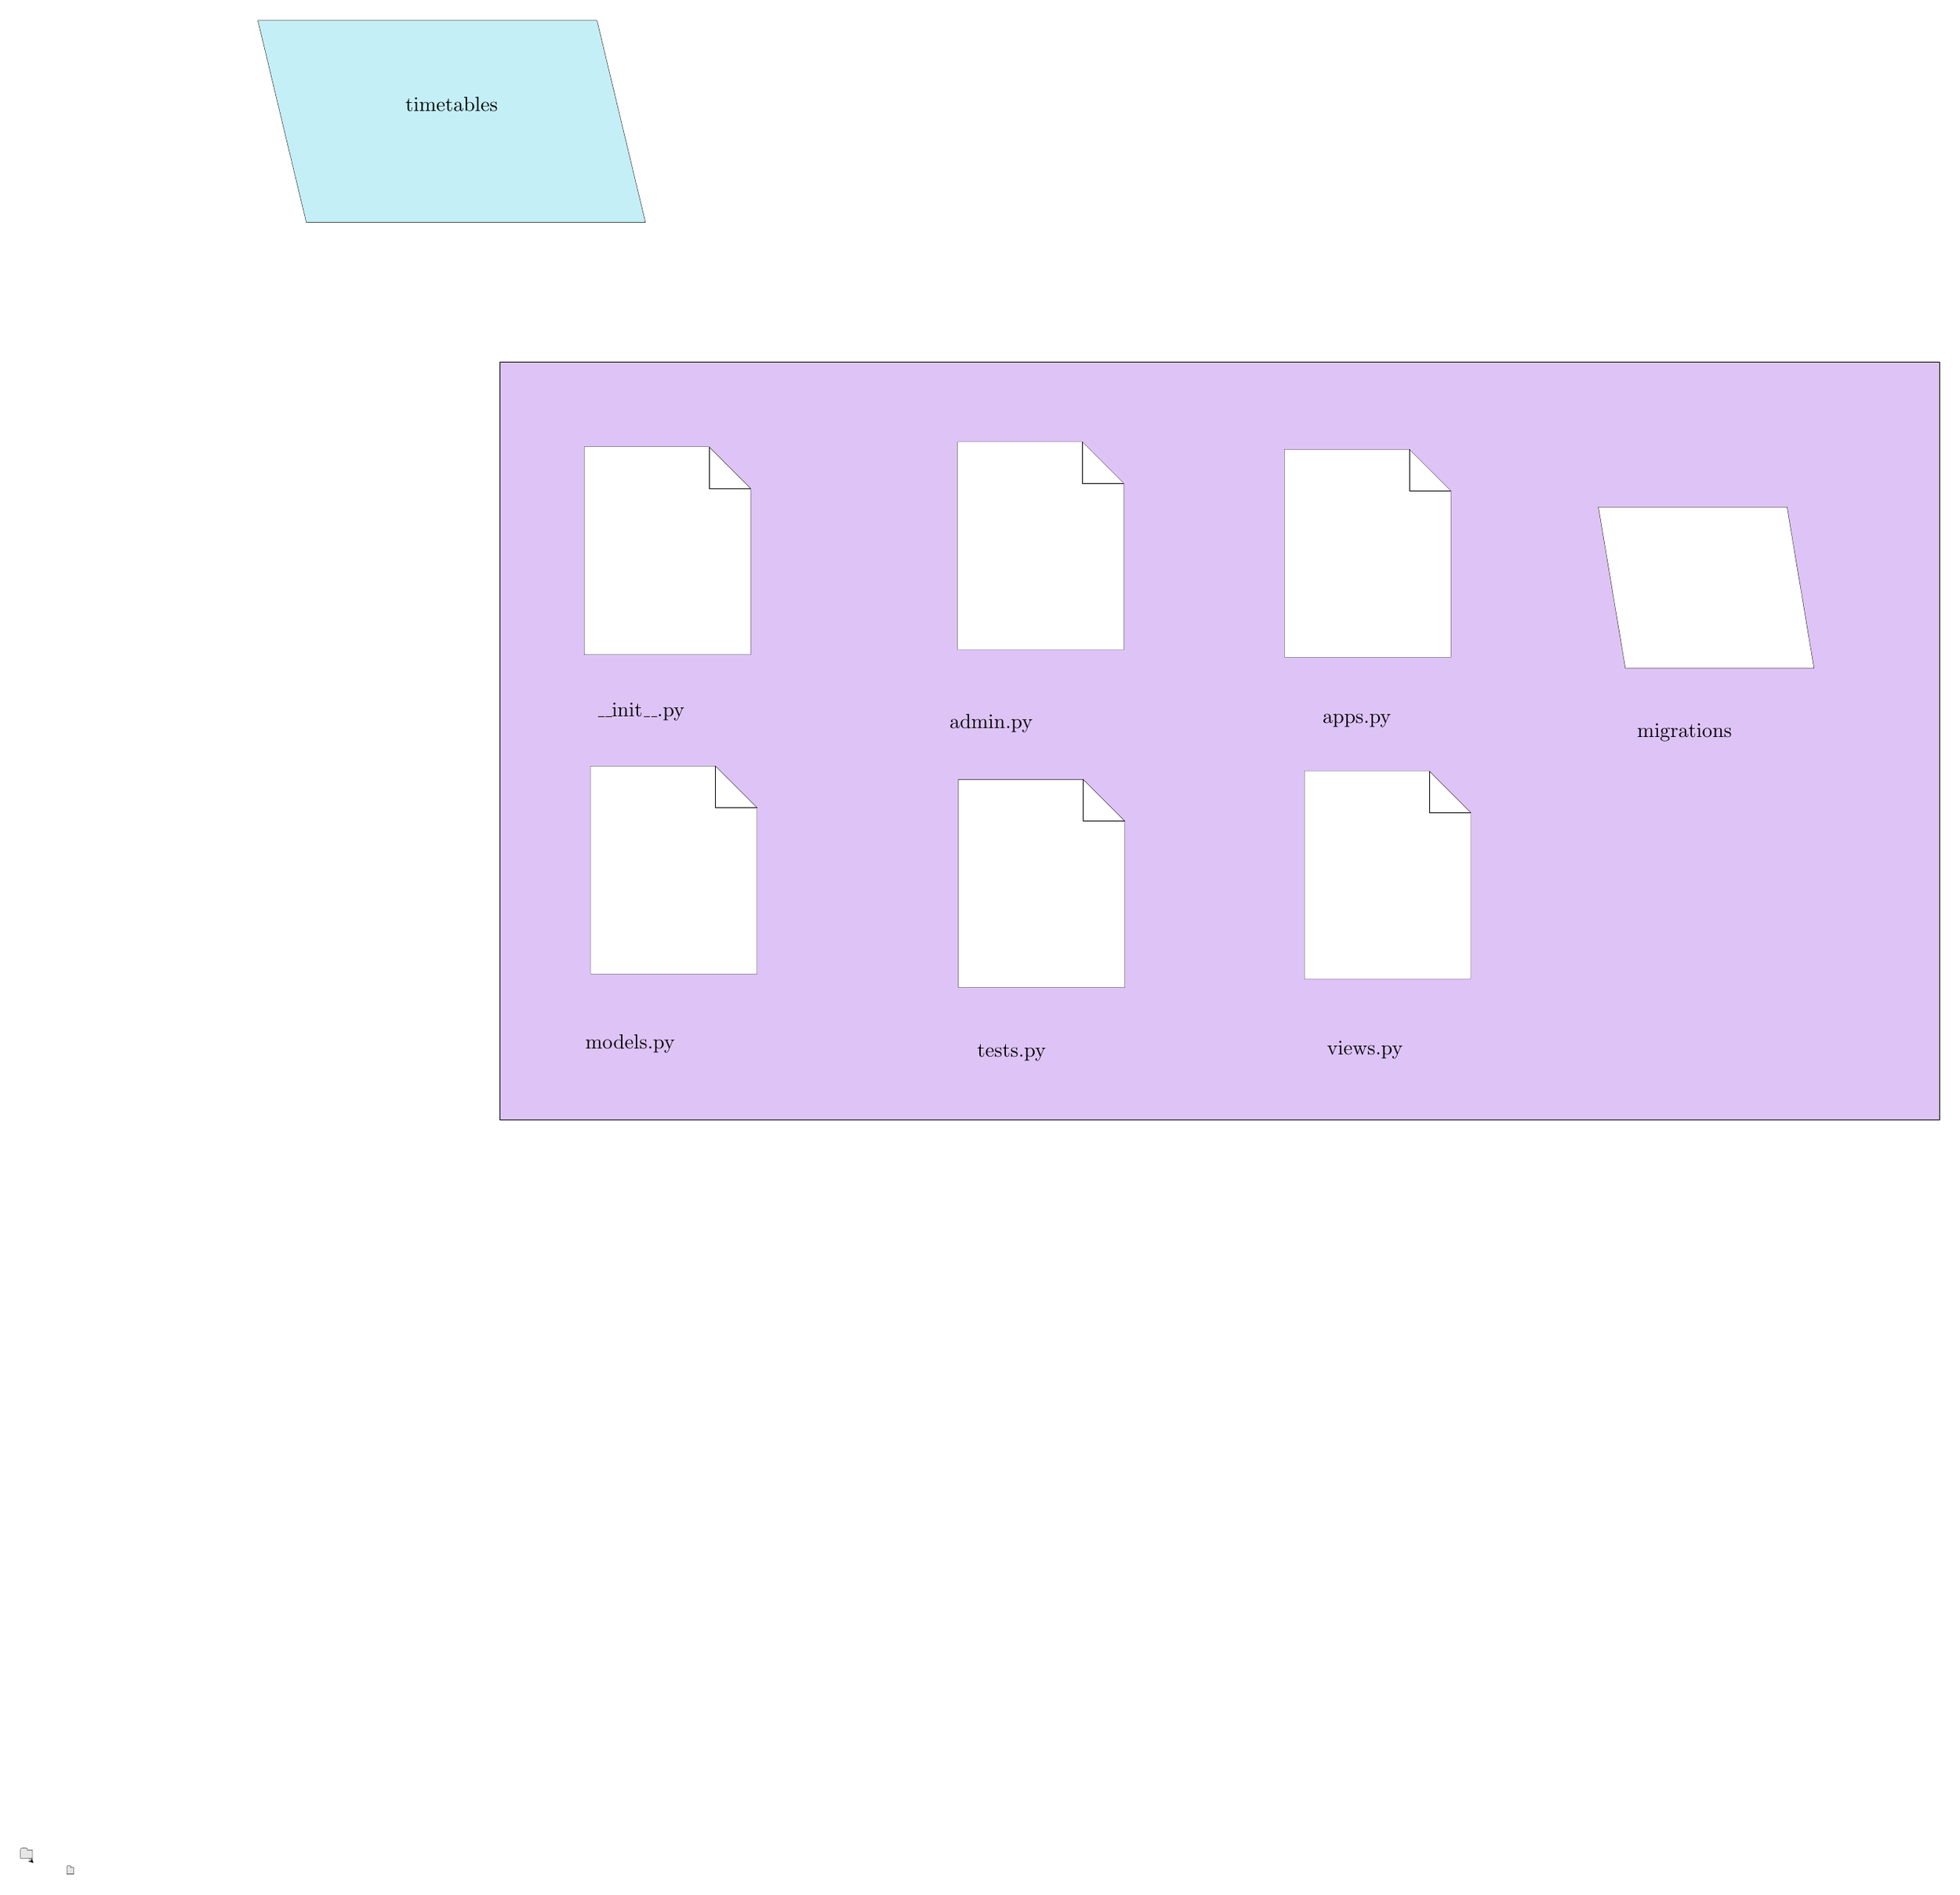
\begin{tikzpicture}
\pgftransformxscale{1.000000}
\pgftransformyscale{-1.000000}
\definecolor{dialinecolor}{rgb}{0.000000, 0.000000, 0.000000}
\pgfsetstrokecolor{dialinecolor}
\definecolor{dialinecolor}{rgb}{1.000000, 1.000000, 1.000000}
\pgfsetfillcolor{dialinecolor}
\pgfsetlinewidth{0.100000\du}
\pgfsetdash{}{0pt}
\pgfsetdash{}{0pt}
\pgfsetbuttcap
\pgfsetmiterjoin
\pgfsetlinewidth{0.100000\du}
\pgfsetbuttcap
\pgfsetmiterjoin
\pgfsetdash{}{0pt}
\definecolor{dialinecolor}{rgb}{0.901961, 0.901961, 0.901961}
\pgfsetfillcolor{dialinecolor}
\pgfpathmoveto{\pgfpoint{5.081250\du}{-33.060000\du}}
\pgfpathcurveto{\pgfpoint{5.081250\du}{-34.050000\du}}{\pgfpoint{5.081250\du}{-34.050000\du}}{\pgfpoint{5.912500\du}{-34.050000\du}}
\pgfpathcurveto{\pgfpoint{6.743750\du}{-34.050000\du}}{\pgfpoint{6.743750\du}{-34.050000\du}}{\pgfpoint{7.575000\du}{-34.050000\du}}
\pgfpathcurveto{\pgfpoint{8.406250\du}{-34.050000\du}}{\pgfpoint{8.406250\du}{-34.050000\du}}{\pgfpoint{8.406250\du}{-33.060000\du}}
\pgfpathcurveto{\pgfpoint{8.406250\du}{-33.060000\du}}{\pgfpoint{10.900000\du}{-33.060000\du}}{\pgfpoint{10.900000\du}{-33.060000\du}}
\pgfpathcurveto{\pgfpoint{10.900000\du}{-33.060000\du}}{\pgfpoint{10.900000\du}{-29.100000\du}}{\pgfpoint{10.900000\du}{-29.100000\du}}
\pgfpathcurveto{\pgfpoint{10.900000\du}{-29.100000\du}}{\pgfpoint{5.081250\du}{-29.100000\du}}{\pgfpoint{5.081250\du}{-29.100000\du}}
\pgfpathcurveto{\pgfpoint{5.081250\du}{-29.100000\du}}{\pgfpoint{5.081250\du}{-32.069999\du}}{\pgfpoint{5.081250\du}{-33.060000\du}}
\pgfusepath{fill}
\definecolor{dialinecolor}{rgb}{0.000000, 0.000000, 0.000000}
\pgfsetstrokecolor{dialinecolor}
\pgfpathmoveto{\pgfpoint{5.081250\du}{-33.060000\du}}
\pgfpathcurveto{\pgfpoint{5.081250\du}{-34.050000\du}}{\pgfpoint{5.081250\du}{-34.050000\du}}{\pgfpoint{5.912500\du}{-34.050000\du}}
\pgfpathcurveto{\pgfpoint{6.743750\du}{-34.050000\du}}{\pgfpoint{6.743750\du}{-34.050000\du}}{\pgfpoint{7.575000\du}{-34.050000\du}}
\pgfpathcurveto{\pgfpoint{8.406250\du}{-34.050000\du}}{\pgfpoint{8.406250\du}{-34.050000\du}}{\pgfpoint{8.406250\du}{-33.060000\du}}
\pgfpathcurveto{\pgfpoint{8.406250\du}{-33.060000\du}}{\pgfpoint{10.900000\du}{-33.060000\du}}{\pgfpoint{10.900000\du}{-33.060000\du}}
\pgfpathcurveto{\pgfpoint{10.900000\du}{-33.060000\du}}{\pgfpoint{10.900000\du}{-29.100000\du}}{\pgfpoint{10.900000\du}{-29.100000\du}}
\pgfpathcurveto{\pgfpoint{10.900000\du}{-29.100000\du}}{\pgfpoint{5.081250\du}{-29.100000\du}}{\pgfpoint{5.081250\du}{-29.100000\du}}
\pgfpathcurveto{\pgfpoint{5.081250\du}{-29.100000\du}}{\pgfpoint{5.081250\du}{-32.069999\du}}{\pgfpoint{5.081250\du}{-33.060000\du}}
\pgfusepath{stroke}
\pgfsetlinewidth{0.010000\du}
\pgfsetbuttcap
\pgfsetmiterjoin
\pgfsetdash{}{0pt}
\definecolor{dialinecolor}{rgb}{0.000000, 0.000000, 0.000000}
\pgfsetstrokecolor{dialinecolor}
\pgfpathmoveto{\pgfpoint{5.081250\du}{-33.060000\du}}
\pgfpathcurveto{\pgfpoint{5.081250\du}{-34.050000\du}}{\pgfpoint{5.081250\du}{-34.050000\du}}{\pgfpoint{5.912500\du}{-34.050000\du}}
\pgfpathcurveto{\pgfpoint{6.743750\du}{-34.050000\du}}{\pgfpoint{6.743750\du}{-34.050000\du}}{\pgfpoint{7.575000\du}{-34.050000\du}}
\pgfpathcurveto{\pgfpoint{8.406250\du}{-34.050000\du}}{\pgfpoint{8.406250\du}{-34.050000\du}}{\pgfpoint{8.406250\du}{-33.060000\du}}
\pgfpathcurveto{\pgfpoint{8.406250\du}{-33.060000\du}}{\pgfpoint{10.900000\du}{-33.060000\du}}{\pgfpoint{10.900000\du}{-33.060000\du}}
\pgfpathcurveto{\pgfpoint{10.900000\du}{-33.060000\du}}{\pgfpoint{10.900000\du}{-29.100000\du}}{\pgfpoint{10.900000\du}{-29.100000\du}}
\pgfpathcurveto{\pgfpoint{10.900000\du}{-29.100000\du}}{\pgfpoint{5.081250\du}{-29.100000\du}}{\pgfpoint{5.081250\du}{-29.100000\du}}
\pgfpathcurveto{\pgfpoint{5.081250\du}{-29.100000\du}}{\pgfpoint{5.081250\du}{-32.069999\du}}{\pgfpoint{5.081250\du}{-33.060000\du}}
\pgfusepath{stroke}
\pgfsetlinewidth{0.100000\du}
\pgfsetbuttcap
\pgfsetmiterjoin
\pgfsetdash{}{0pt}
\definecolor{dialinecolor}{rgb}{0.768627, 0.937255, 0.964706}
\pgfsetfillcolor{dialinecolor}
\fill (5.081250\du,-29.100000\du)--(4.250000\du,-32.564999\du)--(10.068750\du,-32.564999\du)--(10.900000\du,-29.100000\du)--cycle;
\definecolor{dialinecolor}{rgb}{0.000000, 0.000000, 0.000000}
\pgfsetstrokecolor{dialinecolor}
\draw (5.081250\du,-29.100000\du)--(4.250000\du,-32.564999\du)--(10.068750\du,-32.564999\du)--(10.900000\du,-29.100000\du)--cycle;
\pgfsetlinewidth{0.010000\du}
\pgfsetbuttcap
\pgfsetmiterjoin
\pgfsetdash{}{0pt}
\definecolor{dialinecolor}{rgb}{0.000000, 0.000000, 0.000000}
\pgfsetstrokecolor{dialinecolor}
\draw (5.081250\du,-29.100000\du)--(4.250000\du,-32.564999\du)--(10.068750\du,-32.564999\du)--(10.900000\du,-29.100000\du)--cycle;
% setfont left to latex
\definecolor{dialinecolor}{rgb}{0.000000, 0.000000, 0.000000}
\pgfsetstrokecolor{dialinecolor}
\node at (7.575000\du,-31.127500\du){timetables};
\pgfsetlinewidth{0.100000\du}
\pgfsetdash{}{0pt}
\pgfsetdash{}{0pt}
\pgfsetmiterjoin
\definecolor{dialinecolor}{rgb}{0.870588, 0.768627, 0.964706}
\pgfsetfillcolor{dialinecolor}
\fill (8.400000\du,-26.700000\du)--(8.400000\du,-13.700000\du)--(33.100000\du,-13.700000\du)--(33.100000\du,-26.700000\du)--cycle;
\definecolor{dialinecolor}{rgb}{0.000000, 0.000000, 0.000000}
\pgfsetstrokecolor{dialinecolor}
\draw (8.400000\du,-26.700000\du)--(8.400000\du,-13.700000\du)--(33.100000\du,-13.700000\du)--(33.100000\du,-26.700000\du)--cycle;
\pgfsetlinewidth{0.100000\du}
\pgfsetdash{}{0pt}
\pgfsetdash{}{0pt}
\pgfsetbuttcap
{
\definecolor{dialinecolor}{rgb}{0.000000, 0.000000, 0.000000}
\pgfsetfillcolor{dialinecolor}
% was here!!!
\pgfsetarrowsend{stealth}
\definecolor{dialinecolor}{rgb}{0.000000, 0.000000, 0.000000}
\pgfsetstrokecolor{dialinecolor}
\pgfpathmoveto{\pgfpoint{9.331398\du}{-29.051534\du}}
\pgfpatharc{140}{135}{34.537577\du and 34.537577\du}
\pgfusepath{stroke}
}
\pgfsetlinewidth{0.100000\du}
\pgfsetdash{}{0pt}
\pgfsetdash{}{0pt}
\pgfsetbuttcap
\pgfsetmiterjoin
\pgfsetlinewidth{0.100000\du}
\pgfsetbuttcap
\pgfsetmiterjoin
\pgfsetdash{}{0pt}
\definecolor{dialinecolor}{rgb}{1.000000, 1.000000, 1.000000}
\pgfsetfillcolor{dialinecolor}
\fill (9.850000\du,-25.250000\du)--(11.991250\du,-25.250000\du)--(12.705000\du,-24.536250\du)--(12.705000\du,-21.681250\du)--(9.850000\du,-21.681250\du)--cycle;
\definecolor{dialinecolor}{rgb}{0.000000, 0.000000, 0.000000}
\pgfsetstrokecolor{dialinecolor}
\draw (9.850000\du,-25.250000\du)--(11.991250\du,-25.250000\du)--(12.705000\du,-24.536250\du)--(12.705000\du,-21.681250\du)--(9.850000\du,-21.681250\du)--cycle;
\pgfsetbuttcap
\pgfsetmiterjoin
\pgfsetdash{}{0pt}
\definecolor{dialinecolor}{rgb}{0.000000, 0.000000, 0.000000}
\pgfsetstrokecolor{dialinecolor}
\draw (11.991250\du,-25.250000\du)--(11.991250\du,-24.536250\du)--(12.705000\du,-24.536250\du)--(12.705000\du,-24.536250\du);
% setfont left to latex
\definecolor{dialinecolor}{rgb}{0.000000, 0.000000, 0.000000}
\pgfsetstrokecolor{dialinecolor}
\node[anchor=west] at (9.950000\du,-20.700000\du){\_\_init\_\_.py};
\pgfsetlinewidth{0.100000\du}
\pgfsetdash{}{0pt}
\pgfsetdash{}{0pt}
\pgfsetbuttcap
\pgfsetmiterjoin
\pgfsetlinewidth{0.100000\du}
\pgfsetbuttcap
\pgfsetmiterjoin
\pgfsetdash{}{0pt}
\definecolor{dialinecolor}{rgb}{1.000000, 1.000000, 1.000000}
\pgfsetfillcolor{dialinecolor}
\fill (9.960000\du,-19.770000\du)--(12.101250\du,-19.770000\du)--(12.815000\du,-19.056250\du)--(12.815000\du,-16.201250\du)--(9.960000\du,-16.201250\du)--cycle;
\definecolor{dialinecolor}{rgb}{0.000000, 0.000000, 0.000000}
\pgfsetstrokecolor{dialinecolor}
\draw (9.960000\du,-19.770000\du)--(12.101250\du,-19.770000\du)--(12.815000\du,-19.056250\du)--(12.815000\du,-16.201250\du)--(9.960000\du,-16.201250\du)--cycle;
\pgfsetbuttcap
\pgfsetmiterjoin
\pgfsetdash{}{0pt}
\definecolor{dialinecolor}{rgb}{0.000000, 0.000000, 0.000000}
\pgfsetstrokecolor{dialinecolor}
\draw (12.101250\du,-19.770000\du)--(12.101250\du,-19.056250\du)--(12.815000\du,-19.056250\du)--(12.815000\du,-19.056250\du);
% setfont left to latex
\definecolor{dialinecolor}{rgb}{0.000000, 0.000000, 0.000000}
\pgfsetstrokecolor{dialinecolor}
\node[anchor=west] at (9.750000\du,-15.000000\du){models.py};
\pgfsetlinewidth{0.100000\du}
\pgfsetdash{}{0pt}
\pgfsetdash{}{0pt}
\pgfsetbuttcap
\pgfsetmiterjoin
\pgfsetlinewidth{0.100000\du}
\pgfsetbuttcap
\pgfsetmiterjoin
\pgfsetdash{}{0pt}
\definecolor{dialinecolor}{rgb}{1.000000, 1.000000, 1.000000}
\pgfsetfillcolor{dialinecolor}
\fill (21.865000\du,-25.205000\du)--(24.006250\du,-25.205000\du)--(24.720000\du,-24.491250\du)--(24.720000\du,-21.636250\du)--(21.865000\du,-21.636250\du)--cycle;
\definecolor{dialinecolor}{rgb}{0.000000, 0.000000, 0.000000}
\pgfsetstrokecolor{dialinecolor}
\draw (21.865000\du,-25.205000\du)--(24.006250\du,-25.205000\du)--(24.720000\du,-24.491250\du)--(24.720000\du,-21.636250\du)--(21.865000\du,-21.636250\du)--cycle;
\pgfsetbuttcap
\pgfsetmiterjoin
\pgfsetdash{}{0pt}
\definecolor{dialinecolor}{rgb}{0.000000, 0.000000, 0.000000}
\pgfsetstrokecolor{dialinecolor}
\draw (24.006250\du,-25.205000\du)--(24.006250\du,-24.491250\du)--(24.720000\du,-24.491250\du)--(24.720000\du,-24.491250\du);
% setfont left to latex
\definecolor{dialinecolor}{rgb}{0.000000, 0.000000, 0.000000}
\pgfsetstrokecolor{dialinecolor}
\node[anchor=west] at (22.400000\du,-20.550000\du){apps.py};
% setfont left to latex
\definecolor{dialinecolor}{rgb}{0.000000, 0.000000, 0.000000}
\pgfsetstrokecolor{dialinecolor}
\node[anchor=west] at (16.000000\du,-20.500000\du){admin.py};
\pgfsetlinewidth{0.100000\du}
\pgfsetdash{}{0pt}
\pgfsetdash{}{0pt}
\pgfsetbuttcap
\pgfsetmiterjoin
\pgfsetlinewidth{0.100000\du}
\pgfsetbuttcap
\pgfsetmiterjoin
\pgfsetdash{}{0pt}
\definecolor{dialinecolor}{rgb}{1.000000, 1.000000, 1.000000}
\pgfsetfillcolor{dialinecolor}
\fill (16.255000\du,-25.335000\du)--(18.396250\du,-25.335000\du)--(19.110000\du,-24.621250\du)--(19.110000\du,-21.766250\du)--(16.255000\du,-21.766250\du)--cycle;
\definecolor{dialinecolor}{rgb}{0.000000, 0.000000, 0.000000}
\pgfsetstrokecolor{dialinecolor}
\draw (16.255000\du,-25.335000\du)--(18.396250\du,-25.335000\du)--(19.110000\du,-24.621250\du)--(19.110000\du,-21.766250\du)--(16.255000\du,-21.766250\du)--cycle;
\pgfsetbuttcap
\pgfsetmiterjoin
\pgfsetdash{}{0pt}
\definecolor{dialinecolor}{rgb}{0.000000, 0.000000, 0.000000}
\pgfsetstrokecolor{dialinecolor}
\draw (18.396250\du,-25.335000\du)--(18.396250\du,-24.621250\du)--(19.110000\du,-24.621250\du)--(19.110000\du,-24.621250\du);
\pgfsetlinewidth{0.100000\du}
\pgfsetdash{}{0pt}
\pgfsetdash{}{0pt}
\pgfsetbuttcap
\pgfsetmiterjoin
\pgfsetlinewidth{0.100000\du}
\pgfsetbuttcap
\pgfsetmiterjoin
\pgfsetdash{}{0pt}
\definecolor{dialinecolor}{rgb}{1.000000, 1.000000, 1.000000}
\pgfsetfillcolor{dialinecolor}
\fill (16.270000\du,-19.540000\du)--(18.411250\du,-19.540000\du)--(19.125000\du,-18.826250\du)--(19.125000\du,-15.971250\du)--(16.270000\du,-15.971250\du)--cycle;
\definecolor{dialinecolor}{rgb}{0.000000, 0.000000, 0.000000}
\pgfsetstrokecolor{dialinecolor}
\draw (16.270000\du,-19.540000\du)--(18.411250\du,-19.540000\du)--(19.125000\du,-18.826250\du)--(19.125000\du,-15.971250\du)--(16.270000\du,-15.971250\du)--cycle;
\pgfsetbuttcap
\pgfsetmiterjoin
\pgfsetdash{}{0pt}
\definecolor{dialinecolor}{rgb}{0.000000, 0.000000, 0.000000}
\pgfsetstrokecolor{dialinecolor}
\draw (18.411250\du,-19.540000\du)--(18.411250\du,-18.826250\du)--(19.125000\du,-18.826250\du)--(19.125000\du,-18.826250\du);
% setfont left to latex
\definecolor{dialinecolor}{rgb}{0.000000, 0.000000, 0.000000}
\pgfsetstrokecolor{dialinecolor}
\node[anchor=west] at (16.475000\du,-14.850000\du){tests.py};
\pgfsetlinewidth{0.100000\du}
\pgfsetdash{}{0pt}
\pgfsetdash{}{0pt}
\pgfsetbuttcap
\pgfsetmiterjoin
\pgfsetlinewidth{0.100000\du}
\pgfsetbuttcap
\pgfsetmiterjoin
\pgfsetdash{}{0pt}
\definecolor{dialinecolor}{rgb}{1.000000, 1.000000, 1.000000}
\pgfsetfillcolor{dialinecolor}
\fill (22.205000\du,-19.685000\du)--(24.346250\du,-19.685000\du)--(25.060000\du,-18.971250\du)--(25.060000\du,-16.116250\du)--(22.205000\du,-16.116250\du)--cycle;
\definecolor{dialinecolor}{rgb}{0.000000, 0.000000, 0.000000}
\pgfsetstrokecolor{dialinecolor}
\draw (22.205000\du,-19.685000\du)--(24.346250\du,-19.685000\du)--(25.060000\du,-18.971250\du)--(25.060000\du,-16.116250\du)--(22.205000\du,-16.116250\du)--cycle;
\pgfsetbuttcap
\pgfsetmiterjoin
\pgfsetdash{}{0pt}
\definecolor{dialinecolor}{rgb}{0.000000, 0.000000, 0.000000}
\pgfsetstrokecolor{dialinecolor}
\draw (24.346250\du,-19.685000\du)--(24.346250\du,-18.971250\du)--(25.060000\du,-18.971250\du)--(25.060000\du,-18.971250\du);
% setfont left to latex
\definecolor{dialinecolor}{rgb}{0.000000, 0.000000, 0.000000}
\pgfsetstrokecolor{dialinecolor}
\node[anchor=west] at (22.475000\du,-14.900000\du){views.py};
\pgfsetlinewidth{0.100000\du}
\pgfsetdash{}{0pt}
\pgfsetdash{}{0pt}
\pgfsetbuttcap
\pgfsetmiterjoin
\pgfsetlinewidth{0.100000\du}
\pgfsetbuttcap
\pgfsetmiterjoin
\pgfsetdash{}{0pt}
\definecolor{dialinecolor}{rgb}{0.901961, 0.901961, 0.901961}
\pgfsetfillcolor{dialinecolor}
\pgfpathmoveto{\pgfpoint{27.712500\du}{-24.610000\du}}
\pgfpathcurveto{\pgfpoint{27.712500\du}{-25.400000\du}}{\pgfpoint{27.712500\du}{-25.400000\du}}{\pgfpoint{28.175000\du}{-25.400000\du}}
\pgfpathcurveto{\pgfpoint{28.637500\du}{-25.400000\du}}{\pgfpoint{28.637500\du}{-25.400000\du}}{\pgfpoint{29.100000\du}{-25.400000\du}}
\pgfpathcurveto{\pgfpoint{29.562500\du}{-25.400000\du}}{\pgfpoint{29.562500\du}{-25.400000\du}}{\pgfpoint{29.562500\du}{-24.610000\du}}
\pgfpathcurveto{\pgfpoint{29.562500\du}{-24.610000\du}}{\pgfpoint{30.950000\du}{-24.610000\du}}{\pgfpoint{30.950000\du}{-24.610000\du}}
\pgfpathcurveto{\pgfpoint{30.950000\du}{-24.610000\du}}{\pgfpoint{30.950000\du}{-21.450000\du}}{\pgfpoint{30.950000\du}{-21.450000\du}}
\pgfpathcurveto{\pgfpoint{30.950000\du}{-21.450000\du}}{\pgfpoint{27.712500\du}{-21.450000\du}}{\pgfpoint{27.712500\du}{-21.450000\du}}
\pgfpathcurveto{\pgfpoint{27.712500\du}{-21.450000\du}}{\pgfpoint{27.712500\du}{-23.820000\du}}{\pgfpoint{27.712500\du}{-24.610000\du}}
\pgfusepath{fill}
\definecolor{dialinecolor}{rgb}{0.000000, 0.000000, 0.000000}
\pgfsetstrokecolor{dialinecolor}
\pgfpathmoveto{\pgfpoint{27.712500\du}{-24.610000\du}}
\pgfpathcurveto{\pgfpoint{27.712500\du}{-25.400000\du}}{\pgfpoint{27.712500\du}{-25.400000\du}}{\pgfpoint{28.175000\du}{-25.400000\du}}
\pgfpathcurveto{\pgfpoint{28.637500\du}{-25.400000\du}}{\pgfpoint{28.637500\du}{-25.400000\du}}{\pgfpoint{29.100000\du}{-25.400000\du}}
\pgfpathcurveto{\pgfpoint{29.562500\du}{-25.400000\du}}{\pgfpoint{29.562500\du}{-25.400000\du}}{\pgfpoint{29.562500\du}{-24.610000\du}}
\pgfpathcurveto{\pgfpoint{29.562500\du}{-24.610000\du}}{\pgfpoint{30.950000\du}{-24.610000\du}}{\pgfpoint{30.950000\du}{-24.610000\du}}
\pgfpathcurveto{\pgfpoint{30.950000\du}{-24.610000\du}}{\pgfpoint{30.950000\du}{-21.450000\du}}{\pgfpoint{30.950000\du}{-21.450000\du}}
\pgfpathcurveto{\pgfpoint{30.950000\du}{-21.450000\du}}{\pgfpoint{27.712500\du}{-21.450000\du}}{\pgfpoint{27.712500\du}{-21.450000\du}}
\pgfpathcurveto{\pgfpoint{27.712500\du}{-21.450000\du}}{\pgfpoint{27.712500\du}{-23.820000\du}}{\pgfpoint{27.712500\du}{-24.610000\du}}
\pgfusepath{stroke}
\pgfsetlinewidth{0.010000\du}
\pgfsetbuttcap
\pgfsetmiterjoin
\pgfsetdash{}{0pt}
\definecolor{dialinecolor}{rgb}{0.000000, 0.000000, 0.000000}
\pgfsetstrokecolor{dialinecolor}
\pgfpathmoveto{\pgfpoint{27.712500\du}{-24.610000\du}}
\pgfpathcurveto{\pgfpoint{27.712500\du}{-25.400000\du}}{\pgfpoint{27.712500\du}{-25.400000\du}}{\pgfpoint{28.175000\du}{-25.400000\du}}
\pgfpathcurveto{\pgfpoint{28.637500\du}{-25.400000\du}}{\pgfpoint{28.637500\du}{-25.400000\du}}{\pgfpoint{29.100000\du}{-25.400000\du}}
\pgfpathcurveto{\pgfpoint{29.562500\du}{-25.400000\du}}{\pgfpoint{29.562500\du}{-25.400000\du}}{\pgfpoint{29.562500\du}{-24.610000\du}}
\pgfpathcurveto{\pgfpoint{29.562500\du}{-24.610000\du}}{\pgfpoint{30.950000\du}{-24.610000\du}}{\pgfpoint{30.950000\du}{-24.610000\du}}
\pgfpathcurveto{\pgfpoint{30.950000\du}{-24.610000\du}}{\pgfpoint{30.950000\du}{-21.450000\du}}{\pgfpoint{30.950000\du}{-21.450000\du}}
\pgfpathcurveto{\pgfpoint{30.950000\du}{-21.450000\du}}{\pgfpoint{27.712500\du}{-21.450000\du}}{\pgfpoint{27.712500\du}{-21.450000\du}}
\pgfpathcurveto{\pgfpoint{27.712500\du}{-21.450000\du}}{\pgfpoint{27.712500\du}{-23.820000\du}}{\pgfpoint{27.712500\du}{-24.610000\du}}
\pgfusepath{stroke}
\pgfsetlinewidth{0.100000\du}
\pgfsetbuttcap
\pgfsetmiterjoin
\pgfsetdash{}{0pt}
\definecolor{dialinecolor}{rgb}{1.000000, 1.000000, 1.000000}
\pgfsetfillcolor{dialinecolor}
\fill (27.712500\du,-21.450000\du)--(27.250000\du,-24.215000\du)--(30.487500\du,-24.215000\du)--(30.950000\du,-21.450000\du)--cycle;
\definecolor{dialinecolor}{rgb}{0.000000, 0.000000, 0.000000}
\pgfsetstrokecolor{dialinecolor}
\draw (27.712500\du,-21.450000\du)--(27.250000\du,-24.215000\du)--(30.487500\du,-24.215000\du)--(30.950000\du,-21.450000\du)--cycle;
\pgfsetlinewidth{0.010000\du}
\pgfsetbuttcap
\pgfsetmiterjoin
\pgfsetdash{}{0pt}
\definecolor{dialinecolor}{rgb}{0.000000, 0.000000, 0.000000}
\pgfsetstrokecolor{dialinecolor}
\draw (27.712500\du,-21.450000\du)--(27.250000\du,-24.215000\du)--(30.487500\du,-24.215000\du)--(30.950000\du,-21.450000\du)--cycle;
% setfont left to latex
\definecolor{dialinecolor}{rgb}{0.000000, 0.000000, 0.000000}
\pgfsetstrokecolor{dialinecolor}
\node at (29.100000\du,-23.027500\du){};
% setfont left to latex
\definecolor{dialinecolor}{rgb}{0.000000, 0.000000, 0.000000}
\pgfsetstrokecolor{dialinecolor}
\node[anchor=west] at (27.800000\du,-20.350000\du){migrations};
\end{tikzpicture}
}
\caption{Estructura de directorios inicial de una aplicación Django}
\label{djangoappfolders}
\end{figure}

Una vez hemos creado nuestra app, es muy importante añadirla a la configuración de nuestro proyecto y que éste sepa que nuestra app existe. Para ello, sólo tenemos que modificar el fichero \texttt{djangoapp/settings.py} y añadir nuestra app a la lista \texttt{INSTALLED\_APPS}:

\newpage
\begin{minted}{python}
INSTALLED_APPS = [
    'timetables.apps.TimetablesConfig',
    'django.contrib.admin',
    'django.contrib.auth',
    'django.contrib.contenttypes',
    'django.contrib.sessions',
    'django.contrib.messages',
    'django.contrib.staticfiles',
]
\end{minted}

Ya lo tenemos todo preparado para empezar a trabajar en nuestra app.

\subsection{Definiendo los modelos}
\begin{figure}
\centering
\scalebox{.7}{% Graphic for TeX using PGF
% Title: /home/marta/Documents/Git/TFG/Diagrama1.dia
% Creator: Dia v0.97.3
% CreationDate: Fri Sep  8 18:40:19 2017
% For: marta
% \usepackage{tikz}
% The following commands are not supported in PSTricks at present
% We define them conditionally, so when they are implemented,
% this pgf file will use them.
\ifx\du\undefined
  \newlength{\du}
\fi
\setlength{\du}{15\unitlength}
\begin{tikzpicture}
\pgftransformxscale{1.000000}
\pgftransformyscale{-1.000000}
\definecolor{dialinecolor}{rgb}{0.000000, 0.000000, 0.000000}
\pgfsetstrokecolor{dialinecolor}
\definecolor{dialinecolor}{rgb}{1.000000, 1.000000, 1.000000}
\pgfsetfillcolor{dialinecolor}
\pgfsetlinewidth{0.100000\du}
\pgfsetdash{}{0pt}
\definecolor{dialinecolor}{rgb}{1.000000, 1.000000, 1.000000}
\pgfsetfillcolor{dialinecolor}
\fill (4.650000\du,4.950000\du)--(4.650000\du,5.850000\du)--(13.265000\du,5.850000\du)--(13.265000\du,4.950000\du)--cycle;
\definecolor{dialinecolor}{rgb}{0.000000, 0.000000, 0.000000}
\pgfsetstrokecolor{dialinecolor}
\draw (4.650000\du,4.950000\du)--(4.650000\du,5.850000\du)--(13.265000\du,5.850000\du)--(13.265000\du,4.950000\du)--cycle;
% setfont left to latex
\definecolor{dialinecolor}{rgb}{0.000000, 0.000000, 0.000000}
\pgfsetstrokecolor{dialinecolor}
\node at (8.957500\du,5.650000\du){Subject};
\definecolor{dialinecolor}{rgb}{1.000000, 1.000000, 1.000000}
\pgfsetfillcolor{dialinecolor}
\fill (4.650000\du,5.850000\du)--(4.650000\du,14.050000\du)--(13.265000\du,14.050000\du)--(13.265000\du,5.850000\du)--cycle;
\definecolor{dialinecolor}{rgb}{0.000000, 0.000000, 0.000000}
\pgfsetstrokecolor{dialinecolor}
\draw (4.650000\du,5.850000\du)--(4.650000\du,14.050000\du)--(13.265000\du,14.050000\du)--(13.265000\du,5.850000\du)--cycle;
% setfont left to latex
\pgfsetlinewidth{0.010000\du}
\pgfsetmiterjoin
\definecolor{dialinecolor}{rgb}{0.000000, 0.000000, 0.000000}
\pgfsetfillcolor{dialinecolor}
\fill (4.800000\du,6.350000\du)--(4.900000\du,6.500000\du)--(5.000000\du,6.350000\du)--(4.900000\du,6.200000\du)--cycle;
\definecolor{dialinecolor}{rgb}{0.000000, 0.000000, 0.000000}
\pgfsetstrokecolor{dialinecolor}
\node[anchor=west] at (5.100000\du,6.650000\du){ID};
\definecolor{dialinecolor}{rgb}{0.000000, 0.000000, 0.000000}
\pgfsetstrokecolor{dialinecolor}
\node[anchor=west] at (10.220000\du,6.650000\du){Integer};
% setfont left to latex
\pgfsetlinewidth{0.010000\du}
\definecolor{dialinecolor}{rgb}{0.000000, 0.000000, 0.000000}
\pgfsetfillcolor{dialinecolor}
\pgfpathellipse{\pgfpoint{4.900000\du}{7.150000\du}}{\pgfpoint{0.100000\du}{0\du}}{\pgfpoint{0\du}{0.100000\du}}
\pgfusepath{fill}
\definecolor{dialinecolor}{rgb}{0.000000, 0.000000, 0.000000}
\pgfsetstrokecolor{dialinecolor}
\node[anchor=west] at (5.100000\du,7.450000\du){Name};
\definecolor{dialinecolor}{rgb}{0.000000, 0.000000, 0.000000}
\pgfsetstrokecolor{dialinecolor}
\node[anchor=west] at (10.220000\du,7.450000\du){Char};
% setfont left to latex
\pgfsetlinewidth{0.010000\du}
\definecolor{dialinecolor}{rgb}{0.000000, 0.000000, 0.000000}
\pgfsetfillcolor{dialinecolor}
\pgfpathellipse{\pgfpoint{4.900000\du}{7.950000\du}}{\pgfpoint{0.100000\du}{0\du}}{\pgfpoint{0\du}{0.100000\du}}
\pgfusepath{fill}
\definecolor{dialinecolor}{rgb}{0.000000, 0.000000, 0.000000}
\pgfsetstrokecolor{dialinecolor}
\node[anchor=west] at (5.100000\du,8.250000\du){Theory Hours};
\definecolor{dialinecolor}{rgb}{0.000000, 0.000000, 0.000000}
\pgfsetstrokecolor{dialinecolor}
\node[anchor=west] at (10.220000\du,8.250000\du){Integer};
% setfont left to latex
\pgfsetlinewidth{0.010000\du}
\definecolor{dialinecolor}{rgb}{0.000000, 0.000000, 0.000000}
\pgfsetfillcolor{dialinecolor}
\pgfpathellipse{\pgfpoint{4.900000\du}{8.750000\du}}{\pgfpoint{0.100000\du}{0\du}}{\pgfpoint{0\du}{0.100000\du}}
\pgfusepath{fill}
\definecolor{dialinecolor}{rgb}{0.000000, 0.000000, 0.000000}
\pgfsetstrokecolor{dialinecolor}
\node[anchor=west] at (5.100000\du,9.050000\du){Lab Hours};
\definecolor{dialinecolor}{rgb}{0.000000, 0.000000, 0.000000}
\pgfsetstrokecolor{dialinecolor}
\node[anchor=west] at (10.220000\du,9.050000\du){Integer};
% setfont left to latex
\pgfsetlinewidth{0.010000\du}
\definecolor{dialinecolor}{rgb}{0.000000, 0.000000, 0.000000}
\pgfsetfillcolor{dialinecolor}
\pgfpathellipse{\pgfpoint{4.900000\du}{9.550000\du}}{\pgfpoint{0.100000\du}{0\du}}{\pgfpoint{0\du}{0.100000\du}}
\pgfusepath{fill}
\definecolor{dialinecolor}{rgb}{0.000000, 0.000000, 0.000000}
\pgfsetstrokecolor{dialinecolor}
\node[anchor=west] at (5.100000\du,9.850000\du){Acronym};
\definecolor{dialinecolor}{rgb}{0.000000, 0.000000, 0.000000}
\pgfsetstrokecolor{dialinecolor}
\node[anchor=west] at (10.220000\du,9.850000\du){Char};
% setfont left to latex
\pgfsetlinewidth{0.010000\du}
\definecolor{dialinecolor}{rgb}{0.000000, 0.000000, 0.000000}
\pgfsetfillcolor{dialinecolor}
\pgfpathellipse{\pgfpoint{4.900000\du}{10.350000\du}}{\pgfpoint{0.100000\du}{0\du}}{\pgfpoint{0\du}{0.100000\du}}
\pgfusepath{fill}
\definecolor{dialinecolor}{rgb}{0.000000, 0.000000, 0.000000}
\pgfsetstrokecolor{dialinecolor}
\node[anchor=west] at (5.100000\du,10.650000\du){Speciality};
\definecolor{dialinecolor}{rgb}{0.000000, 0.000000, 0.000000}
\pgfsetstrokecolor{dialinecolor}
\node[anchor=west] at (10.220000\du,10.650000\du){Char};
% setfont left to latex
\pgfsetlinewidth{0.010000\du}
\definecolor{dialinecolor}{rgb}{0.000000, 0.000000, 0.000000}
\pgfsetfillcolor{dialinecolor}
\pgfpathellipse{\pgfpoint{4.900000\du}{11.150000\du}}{\pgfpoint{0.100000\du}{0\du}}{\pgfpoint{0\du}{0.100000\du}}
\pgfusepath{fill}
\definecolor{dialinecolor}{rgb}{0.000000, 0.000000, 0.000000}
\pgfsetstrokecolor{dialinecolor}
\node[anchor=west] at (5.100000\du,11.450000\du){Year};
\definecolor{dialinecolor}{rgb}{0.000000, 0.000000, 0.000000}
\pgfsetstrokecolor{dialinecolor}
\node[anchor=west] at (10.220000\du,11.450000\du){Integer};
% setfont left to latex
\pgfsetlinewidth{0.010000\du}
\definecolor{dialinecolor}{rgb}{0.000000, 0.000000, 0.000000}
\pgfsetfillcolor{dialinecolor}
\pgfpathellipse{\pgfpoint{4.900000\du}{11.950000\du}}{\pgfpoint{0.100000\du}{0\du}}{\pgfpoint{0\du}{0.100000\du}}
\pgfusepath{fill}
\definecolor{dialinecolor}{rgb}{0.000000, 0.000000, 0.000000}
\pgfsetstrokecolor{dialinecolor}
\node[anchor=west] at (5.100000\du,12.250000\du){Semester};
\definecolor{dialinecolor}{rgb}{0.000000, 0.000000, 0.000000}
\pgfsetstrokecolor{dialinecolor}
\node[anchor=west] at (10.220000\du,12.250000\du){Integer};
% setfont left to latex
\pgfsetlinewidth{0.010000\du}
\definecolor{dialinecolor}{rgb}{0.000000, 0.000000, 0.000000}
\pgfsetfillcolor{dialinecolor}
\pgfpathellipse{\pgfpoint{4.900000\du}{12.750000\du}}{\pgfpoint{0.100000\du}{0\du}}{\pgfpoint{0\du}{0.100000\du}}
\pgfusepath{fill}
\definecolor{dialinecolor}{rgb}{0.000000, 0.000000, 0.000000}
\pgfsetstrokecolor{dialinecolor}
\node[anchor=west] at (5.100000\du,13.050000\du){Degree};
\definecolor{dialinecolor}{rgb}{0.000000, 0.000000, 0.000000}
\pgfsetstrokecolor{dialinecolor}
\node[anchor=west] at (10.220000\du,13.050000\du){Char};
% setfont left to latex
\pgfsetlinewidth{0.010000\du}
\definecolor{dialinecolor}{rgb}{0.000000, 0.000000, 0.000000}
\pgfsetfillcolor{dialinecolor}
\pgfpathellipse{\pgfpoint{4.900000\du}{13.550000\du}}{\pgfpoint{0.100000\du}{0\du}}{\pgfpoint{0\du}{0.100000\du}}
\pgfusepath{fill}
\definecolor{dialinecolor}{rgb}{0.000000, 0.000000, 0.000000}
\pgfsetstrokecolor{dialinecolor}
\node[anchor=west] at (5.100000\du,13.850000\du){Students};
\definecolor{dialinecolor}{rgb}{0.000000, 0.000000, 0.000000}
\pgfsetstrokecolor{dialinecolor}
\node[anchor=west] at (10.220000\du,13.850000\du){Integer};
\pgfsetlinewidth{0.100000\du}
\pgfsetdash{}{0pt}
\definecolor{dialinecolor}{rgb}{1.000000, 1.000000, 1.000000}
\pgfsetfillcolor{dialinecolor}
\fill (4.600000\du,19.000000\du)--(4.600000\du,19.900000\du)--(12.445000\du,19.900000\du)--(12.445000\du,19.000000\du)--cycle;
\definecolor{dialinecolor}{rgb}{0.000000, 0.000000, 0.000000}
\pgfsetstrokecolor{dialinecolor}
\draw (4.600000\du,19.000000\du)--(4.600000\du,19.900000\du)--(12.445000\du,19.900000\du)--(12.445000\du,19.000000\du)--cycle;
% setfont left to latex
\definecolor{dialinecolor}{rgb}{0.000000, 0.000000, 0.000000}
\pgfsetstrokecolor{dialinecolor}
\node at (8.522500\du,19.700000\du){Classroom};
\definecolor{dialinecolor}{rgb}{1.000000, 1.000000, 1.000000}
\pgfsetfillcolor{dialinecolor}
\fill (4.600000\du,19.900000\du)--(4.600000\du,23.300000\du)--(12.445000\du,23.300000\du)--(12.445000\du,19.900000\du)--cycle;
\definecolor{dialinecolor}{rgb}{0.000000, 0.000000, 0.000000}
\pgfsetstrokecolor{dialinecolor}
\draw (4.600000\du,19.900000\du)--(4.600000\du,23.300000\du)--(12.445000\du,23.300000\du)--(12.445000\du,19.900000\du)--cycle;
% setfont left to latex
\pgfsetlinewidth{0.010000\du}
\pgfsetmiterjoin
\definecolor{dialinecolor}{rgb}{0.000000, 0.000000, 0.000000}
\pgfsetfillcolor{dialinecolor}
\fill (4.750000\du,20.400000\du)--(4.850000\du,20.550000\du)--(4.950000\du,20.400000\du)--(4.850000\du,20.250000\du)--cycle;
\definecolor{dialinecolor}{rgb}{0.000000, 0.000000, 0.000000}
\pgfsetstrokecolor{dialinecolor}
\node[anchor=west] at (5.050000\du,20.700000\du){ID};
\definecolor{dialinecolor}{rgb}{0.000000, 0.000000, 0.000000}
\pgfsetstrokecolor{dialinecolor}
\node[anchor=west] at (9.400000\du,20.700000\du){Integer};
% setfont left to latex
\pgfsetlinewidth{0.010000\du}
\definecolor{dialinecolor}{rgb}{0.000000, 0.000000, 0.000000}
\pgfsetfillcolor{dialinecolor}
\pgfpathellipse{\pgfpoint{4.850000\du}{21.200000\du}}{\pgfpoint{0.100000\du}{0\du}}{\pgfpoint{0\du}{0.100000\du}}
\pgfusepath{fill}
\definecolor{dialinecolor}{rgb}{0.000000, 0.000000, 0.000000}
\pgfsetstrokecolor{dialinecolor}
\node[anchor=west] at (5.050000\du,21.500000\du){Name};
\definecolor{dialinecolor}{rgb}{0.000000, 0.000000, 0.000000}
\pgfsetstrokecolor{dialinecolor}
\node[anchor=west] at (9.400000\du,21.500000\du){Char};
% setfont left to latex
\pgfsetlinewidth{0.010000\du}
\definecolor{dialinecolor}{rgb}{0.000000, 0.000000, 0.000000}
\pgfsetfillcolor{dialinecolor}
\pgfpathellipse{\pgfpoint{4.850000\du}{22.000000\du}}{\pgfpoint{0.100000\du}{0\du}}{\pgfpoint{0\du}{0.100000\du}}
\pgfusepath{fill}
\definecolor{dialinecolor}{rgb}{0.000000, 0.000000, 0.000000}
\pgfsetstrokecolor{dialinecolor}
\node[anchor=west] at (5.050000\du,22.300000\du){Capacity};
\definecolor{dialinecolor}{rgb}{0.000000, 0.000000, 0.000000}
\pgfsetstrokecolor{dialinecolor}
\node[anchor=west] at (9.400000\du,22.300000\du){Char};
% setfont left to latex
\pgfsetlinewidth{0.010000\du}
\definecolor{dialinecolor}{rgb}{0.000000, 0.000000, 0.000000}
\pgfsetfillcolor{dialinecolor}
\pgfpathellipse{\pgfpoint{4.850000\du}{22.800000\du}}{\pgfpoint{0.100000\du}{0\du}}{\pgfpoint{0\du}{0.100000\du}}
\pgfusepath{fill}
\definecolor{dialinecolor}{rgb}{0.000000, 0.000000, 0.000000}
\pgfsetstrokecolor{dialinecolor}
\node[anchor=west] at (5.050000\du,23.100000\du){IsPractice};
\definecolor{dialinecolor}{rgb}{0.000000, 0.000000, 0.000000}
\pgfsetstrokecolor{dialinecolor}
\node[anchor=west] at (9.400000\du,23.100000\du){Char};
\pgfsetlinewidth{0.100000\du}
\pgfsetdash{}{0pt}
\definecolor{dialinecolor}{rgb}{1.000000, 1.000000, 1.000000}
\pgfsetfillcolor{dialinecolor}
\fill (3.900000\du,28.150000\du)--(3.900000\du,29.050000\du)--(12.900000\du,29.050000\du)--(12.900000\du,28.150000\du)--cycle;
\definecolor{dialinecolor}{rgb}{0.000000, 0.000000, 0.000000}
\pgfsetstrokecolor{dialinecolor}
\draw (3.900000\du,28.150000\du)--(3.900000\du,29.050000\du)--(12.900000\du,29.050000\du)--(12.900000\du,28.150000\du)--cycle;
% setfont left to latex
\definecolor{dialinecolor}{rgb}{0.000000, 0.000000, 0.000000}
\pgfsetstrokecolor{dialinecolor}
\node at (8.400000\du,28.850000\du){Group};
\definecolor{dialinecolor}{rgb}{1.000000, 1.000000, 1.000000}
\pgfsetfillcolor{dialinecolor}
\fill (3.900000\du,29.050000\du)--(3.900000\du,35.650000\du)--(12.900000\du,35.650000\du)--(12.900000\du,29.050000\du)--cycle;
\definecolor{dialinecolor}{rgb}{0.000000, 0.000000, 0.000000}
\pgfsetstrokecolor{dialinecolor}
\draw (3.900000\du,29.050000\du)--(3.900000\du,35.650000\du)--(12.900000\du,35.650000\du)--(12.900000\du,29.050000\du)--cycle;
% setfont left to latex
\pgfsetlinewidth{0.010000\du}
\pgfsetmiterjoin
\definecolor{dialinecolor}{rgb}{0.000000, 0.000000, 0.000000}
\pgfsetfillcolor{dialinecolor}
\fill (4.050000\du,29.550000\du)--(4.150000\du,29.700000\du)--(4.250000\du,29.550000\du)--(4.150000\du,29.400000\du)--cycle;
\definecolor{dialinecolor}{rgb}{0.000000, 0.000000, 0.000000}
\pgfsetstrokecolor{dialinecolor}
\node[anchor=west] at (4.350000\du,29.850000\du){ID};
\definecolor{dialinecolor}{rgb}{0.000000, 0.000000, 0.000000}
\pgfsetstrokecolor{dialinecolor}
\node[anchor=west] at (8.700000\du,29.850000\du){Integer};
% setfont left to latex
\pgfsetlinewidth{0.010000\du}
\definecolor{dialinecolor}{rgb}{0.000000, 0.000000, 0.000000}
\pgfsetfillcolor{dialinecolor}
\pgfpathellipse{\pgfpoint{4.150000\du}{30.350000\du}}{\pgfpoint{0.100000\du}{0\du}}{\pgfpoint{0\du}{0.100000\du}}
\pgfusepath{fill}
\definecolor{dialinecolor}{rgb}{0.000000, 0.000000, 0.000000}
\pgfsetstrokecolor{dialinecolor}
\node[anchor=west] at (4.350000\du,30.650000\du){Name};
\definecolor{dialinecolor}{rgb}{0.000000, 0.000000, 0.000000}
\pgfsetstrokecolor{dialinecolor}
\node[anchor=west] at (8.700000\du,30.650000\du){Char};
% setfont left to latex
\pgfsetlinewidth{0.010000\du}
\definecolor{dialinecolor}{rgb}{0.000000, 0.000000, 0.000000}
\pgfsetfillcolor{dialinecolor}
\pgfpathellipse{\pgfpoint{4.150000\du}{31.150000\du}}{\pgfpoint{0.100000\du}{0\du}}{\pgfpoint{0\du}{0.100000\du}}
\pgfusepath{fill}
\definecolor{dialinecolor}{rgb}{0.000000, 0.000000, 0.000000}
\pgfsetstrokecolor{dialinecolor}
\node[anchor=west] at (4.350000\du,31.450000\du){Shift};
\definecolor{dialinecolor}{rgb}{0.000000, 0.000000, 0.000000}
\pgfsetstrokecolor{dialinecolor}
\node[anchor=west] at (8.700000\du,31.450000\du){Char};
% setfont left to latex
\pgfsetlinewidth{0.010000\du}
\definecolor{dialinecolor}{rgb}{0.000000, 0.000000, 0.000000}
\pgfsetfillcolor{dialinecolor}
\pgfpathellipse{\pgfpoint{4.150000\du}{31.950000\du}}{\pgfpoint{0.100000\du}{0\du}}{\pgfpoint{0\du}{0.100000\du}}
\pgfusepath{fill}
\definecolor{dialinecolor}{rgb}{0.000000, 0.000000, 0.000000}
\pgfsetstrokecolor{dialinecolor}
\node[anchor=west] at (4.350000\du,32.250000\du){Year};
\definecolor{dialinecolor}{rgb}{0.000000, 0.000000, 0.000000}
\pgfsetstrokecolor{dialinecolor}
\node[anchor=west] at (8.700000\du,32.250000\du){Integer};
% setfont left to latex
\pgfsetlinewidth{0.010000\du}
\definecolor{dialinecolor}{rgb}{0.000000, 0.000000, 0.000000}
\pgfsetfillcolor{dialinecolor}
\pgfpathellipse{\pgfpoint{4.150000\du}{32.750000\du}}{\pgfpoint{0.100000\du}{0\du}}{\pgfpoint{0\du}{0.100000\du}}
\pgfusepath{fill}
\definecolor{dialinecolor}{rgb}{0.000000, 0.000000, 0.000000}
\pgfsetstrokecolor{dialinecolor}
\node[anchor=west] at (4.350000\du,33.050000\du){Degree};
\definecolor{dialinecolor}{rgb}{0.000000, 0.000000, 0.000000}
\pgfsetstrokecolor{dialinecolor}
\node[anchor=west] at (8.700000\du,33.050000\du){Char};
% setfont left to latex
\pgfsetlinewidth{0.010000\du}
\definecolor{dialinecolor}{rgb}{0.000000, 0.000000, 0.000000}
\pgfsetfillcolor{dialinecolor}
\pgfpathellipse{\pgfpoint{4.150000\du}{33.550000\du}}{\pgfpoint{0.100000\du}{0\du}}{\pgfpoint{0\du}{0.100000\du}}
\pgfusepath{fill}
\definecolor{dialinecolor}{rgb}{0.000000, 0.000000, 0.000000}
\pgfsetstrokecolor{dialinecolor}
\node[anchor=west] at (4.350000\du,33.850000\du){Speciality};
\definecolor{dialinecolor}{rgb}{0.000000, 0.000000, 0.000000}
\pgfsetstrokecolor{dialinecolor}
\node[anchor=west] at (8.700000\du,33.850000\du){Char};
% setfont left to latex
\pgfsetlinewidth{0.010000\du}
\definecolor{dialinecolor}{rgb}{0.000000, 0.000000, 0.000000}
\pgfsetfillcolor{dialinecolor}
\pgfpathellipse{\pgfpoint{4.150000\du}{34.350000\du}}{\pgfpoint{0.100000\du}{0\du}}{\pgfpoint{0\du}{0.100000\du}}
\pgfusepath{fill}
\definecolor{dialinecolor}{rgb}{0.000000, 0.000000, 0.000000}
\pgfsetstrokecolor{dialinecolor}
\node[anchor=west] at (4.350000\du,34.650000\du){Semester};
\definecolor{dialinecolor}{rgb}{0.000000, 0.000000, 0.000000}
\pgfsetstrokecolor{dialinecolor}
\node[anchor=west] at (8.700000\du,34.650000\du){Char};
% setfont left to latex
\pgfsetlinewidth{0.010000\du}
\definecolor{dialinecolor}{rgb}{0.000000, 0.000000, 0.000000}
\pgfsetfillcolor{dialinecolor}
\pgfpathellipse{\pgfpoint{4.150000\du}{35.150000\du}}{\pgfpoint{0.100000\du}{0\du}}{\pgfpoint{0\du}{0.100000\du}}
\pgfusepath{fill}
\definecolor{dialinecolor}{rgb}{0.000000, 0.000000, 0.000000}
\pgfsetstrokecolor{dialinecolor}
\node[anchor=west] at (4.350000\du,35.450000\du){Classroom};
\definecolor{dialinecolor}{rgb}{0.000000, 0.000000, 0.000000}
\pgfsetstrokecolor{dialinecolor}
\node[anchor=west] at (8.700000\du,35.450000\du){ForeignKey};
\pgfsetlinewidth{0.100000\du}
\pgfsetdash{}{0pt}
\definecolor{dialinecolor}{rgb}{1.000000, 1.000000, 1.000000}
\pgfsetfillcolor{dialinecolor}
\fill (18.050000\du,14.550000\du)--(18.050000\du,15.450000\du)--(26.665000\du,15.450000\du)--(26.665000\du,14.550000\du)--cycle;
\definecolor{dialinecolor}{rgb}{0.000000, 0.000000, 0.000000}
\pgfsetstrokecolor{dialinecolor}
\draw (18.050000\du,14.550000\du)--(18.050000\du,15.450000\du)--(26.665000\du,15.450000\du)--(26.665000\du,14.550000\du)--cycle;
% setfont left to latex
\definecolor{dialinecolor}{rgb}{0.000000, 0.000000, 0.000000}
\pgfsetstrokecolor{dialinecolor}
\node at (22.357500\du,15.250000\du){SubjectClassroom};
\definecolor{dialinecolor}{rgb}{1.000000, 1.000000, 1.000000}
\pgfsetfillcolor{dialinecolor}
\fill (18.050000\du,15.450000\du)--(18.050000\du,18.050000\du)--(26.665000\du,18.050000\du)--(26.665000\du,15.450000\du)--cycle;
\definecolor{dialinecolor}{rgb}{0.000000, 0.000000, 0.000000}
\pgfsetstrokecolor{dialinecolor}
\draw (18.050000\du,15.450000\du)--(18.050000\du,18.050000\du)--(26.665000\du,18.050000\du)--(26.665000\du,15.450000\du)--cycle;
% setfont left to latex
\pgfsetlinewidth{0.010000\du}
\pgfsetmiterjoin
\definecolor{dialinecolor}{rgb}{0.000000, 0.000000, 0.000000}
\pgfsetfillcolor{dialinecolor}
\fill (18.200000\du,15.950000\du)--(18.300000\du,16.100000\du)--(18.400000\du,15.950000\du)--(18.300000\du,15.800000\du)--cycle;
\definecolor{dialinecolor}{rgb}{0.000000, 0.000000, 0.000000}
\pgfsetstrokecolor{dialinecolor}
\node[anchor=west] at (18.500000\du,16.250000\du){ID};
\definecolor{dialinecolor}{rgb}{0.000000, 0.000000, 0.000000}
\pgfsetstrokecolor{dialinecolor}
\node[anchor=west] at (22.465000\du,16.250000\du){Integer};
% setfont left to latex
\pgfsetlinewidth{0.010000\du}
\definecolor{dialinecolor}{rgb}{0.000000, 0.000000, 0.000000}
\pgfsetfillcolor{dialinecolor}
\pgfpathellipse{\pgfpoint{18.300000\du}{16.750000\du}}{\pgfpoint{0.100000\du}{0\du}}{\pgfpoint{0\du}{0.100000\du}}
\pgfusepath{fill}
\definecolor{dialinecolor}{rgb}{0.000000, 0.000000, 0.000000}
\pgfsetstrokecolor{dialinecolor}
\node[anchor=west] at (18.500000\du,17.050000\du){Subject};
\definecolor{dialinecolor}{rgb}{0.000000, 0.000000, 0.000000}
\pgfsetstrokecolor{dialinecolor}
\node[anchor=west] at (22.465000\du,17.050000\du){ForeignKey};
% setfont left to latex
\pgfsetlinewidth{0.010000\du}
\definecolor{dialinecolor}{rgb}{0.000000, 0.000000, 0.000000}
\pgfsetfillcolor{dialinecolor}
\pgfpathellipse{\pgfpoint{18.300000\du}{17.550000\du}}{\pgfpoint{0.100000\du}{0\du}}{\pgfpoint{0\du}{0.100000\du}}
\pgfusepath{fill}
\definecolor{dialinecolor}{rgb}{0.000000, 0.000000, 0.000000}
\pgfsetstrokecolor{dialinecolor}
\node[anchor=west] at (18.500000\du,17.850000\du){Classroom};
\definecolor{dialinecolor}{rgb}{0.000000, 0.000000, 0.000000}
\pgfsetstrokecolor{dialinecolor}
\node[anchor=west] at (22.465000\du,17.850000\du){ForeignKey};
\pgfsetlinewidth{0.100000\du}
\pgfsetdash{}{0pt}
\pgfsetdash{}{0pt}
\pgfsetmiterjoin
\pgfsetbuttcap
{
\definecolor{dialinecolor}{rgb}{0.000000, 0.000000, 0.000000}
\pgfsetfillcolor{dialinecolor}
% was here!!!
\pgfsetarrowsend{stealth}
{\pgfsetcornersarced{\pgfpoint{0.000000\du}{0.000000\du}}\definecolor{dialinecolor}{rgb}{0.000000, 0.000000, 0.000000}
\pgfsetstrokecolor{dialinecolor}
\draw (8.650000\du,28.150000\du)--(8.650000\du,25.735518\du)--(8.649747\du,25.735518\du)--(8.649747\du,23.321035\du);
}}
% setfont left to latex
\definecolor{dialinecolor}{rgb}{0.000000, 0.000000, 0.000000}
\pgfsetstrokecolor{dialinecolor}
\node[anchor=west] at (8.950000\du,27.850000\du){n};
\definecolor{dialinecolor}{rgb}{0.000000, 0.000000, 0.000000}
\pgfsetstrokecolor{dialinecolor}
\node[anchor=west] at (8.949747\du,24.321035\du){1};
\pgfsetlinewidth{0.100000\du}
\pgfsetdash{}{0pt}
\pgfsetdash{}{0pt}
\pgfsetmiterjoin
\pgfsetbuttcap
{
\definecolor{dialinecolor}{rgb}{0.000000, 0.000000, 0.000000}
\pgfsetfillcolor{dialinecolor}
% was here!!!
\pgfsetarrowsend{stealth}
{\pgfsetcornersarced{\pgfpoint{0.000000\du}{0.000000\du}}\definecolor{dialinecolor}{rgb}{0.000000, 0.000000, 0.000000}
\pgfsetstrokecolor{dialinecolor}
\draw (12.452452\du,22.130246\du)--(15.251226\du,22.130246\du)--(15.251226\du,17.550000\du)--(18.050000\du,17.550000\du);
}}
% setfont left to latex
\definecolor{dialinecolor}{rgb}{0.000000, 0.000000, 0.000000}
\pgfsetstrokecolor{dialinecolor}
\node[anchor=west] at (12.752452\du,21.830246\du){1};
\definecolor{dialinecolor}{rgb}{0.000000, 0.000000, 0.000000}
\pgfsetstrokecolor{dialinecolor}
\node[anchor=east] at (17.750000\du,17.250000\du){n};
\pgfsetlinewidth{0.100000\du}
\pgfsetdash{}{0pt}
\pgfsetdash{}{0pt}
\pgfsetmiterjoin
\pgfsetbuttcap
{
\definecolor{dialinecolor}{rgb}{0.000000, 0.000000, 0.000000}
\pgfsetfillcolor{dialinecolor}
% was here!!!
\pgfsetarrowsend{stealth}
{\pgfsetcornersarced{\pgfpoint{0.000000\du}{0.000000\du}}\definecolor{dialinecolor}{rgb}{0.000000, 0.000000, 0.000000}
\pgfsetstrokecolor{dialinecolor}
\draw (13.335379\du,10.805594\du)--(15.692689\du,10.805594\du)--(15.692689\du,15.950000\du)--(18.050000\du,15.950000\du);
}}
% setfont left to latex
\definecolor{dialinecolor}{rgb}{0.000000, 0.000000, 0.000000}
\pgfsetstrokecolor{dialinecolor}
\node[anchor=west] at (13.635379\du,10.505594\du){1};
\definecolor{dialinecolor}{rgb}{0.000000, 0.000000, 0.000000}
\pgfsetstrokecolor{dialinecolor}
\node[anchor=east] at (17.750000\du,15.650000\du){n};
\end{tikzpicture}
}
\caption{Estructura de tablas en la base de datos}
\label{djangomodels}
\end{figure}

En la \hyperref[djangomodels]{Figura \ref*{djangomodels}} podemos ver el modelo de de base de datos que he diseñado. El diseño que muestro es el de tablas SQL final, pero del diseño a la implementación en \texttt{Django} hay algunas cosas que cambian, ya que \texttt{Django} dispone de un \textit{Object-Relational Mapping} (ORM) \cite{orm}. Un \textit{Object-Relational Mapping} es una herramienta que convierte clases de objectos en tablas SQL. Así, nos abstraemos del concepto de tabla y la concebimos e implementamos como objetos. Por debajo, el \textit{Object-Relational Mapping} crea las tablas y relaciones SQL.

Respecto al modelo de bases de datos definido, la verdad es que no lo tuve muy difícil: he hecho una tabla para cada tipo de dato que almacenábamos en CSV antes de hacer la interfaz.

\begin{enumerate}[---]
    \item \textbf{Asignatura}: en este modelo, guardo todos los datos relativos a una asignatura, y además, las clases de prácticas en las que una asignatura puede impartirse.

Todos los campos son campos SQL normales, menos la relación con el de clases. El campo en el que guardo las clases en las que puede impartirse una asignatura es un campo especial de \texttt{Django} llamado \texttt{ManyToManyField}. Este campo es, por así decirlo, una lista de \textit{foreign keys} a la tabla \texttt{Classroom}. En el SQL normal es imposible hacer algo así, de hecho, \textbf{rompe la primera forma normal} en la normalización de bases de datos: cada campo debe tener un único valor (no una lista). Entonces, ¿cómo es esto posible? En realidad \texttt{Django} no está tan mal hecho como para hacer bases de datos con mala calidad. Cuando le especificamos a \texttt{Django} que haga un \texttt{ManyToManyField}, crea por debajo una nueva tabla en la que guardar dicha relación.

    \item \textbf{Clase}: en este modelo, guardo todos los datos relativos a un aula. Aunque en el modelo de clases Python inicial se separó entre clase de prácticas y clase de teoría, no tenía tanto sentido hacer esta separación en el modelo de base de datos. Tanto la clase de prácticas como la de teoría tenían los mismos campos y, lo único que he hecho para diferenciarlas es añadir un campo al modelo para indicar si una clase es de prácticas o o no. De hecho, con esta definición del modelo he podido definir clases que son a la vez de teoría y de prácticas. Por ejemplo, las prácticas de la asignatura \textit{Álgebra Lineal y Métodos Discretos} del Grado en Ingeniería Informática pueden hacerse en las aulas de la planta 1, al igual que otras tantas asignaturas. Pero todas las clases de teoría que se imparten en tercero y en cuarto curso del Grado en Ingeniería Informática son en la planta 1 también. Por tanto, el campo \texttt{ispractice} puede tomar los valores \texttt{Yes}, \texttt{No} y \texttt{Both}


    \item \textbf{Grupo}: en este modelo, guardo todos los datos relativos a un grupo, además de los cuatrimestres en los que ``existe'' un grupo. Esto es necesario debido a que hay grupos que sólo existen en un determinado cuatrimestre. Por ejemplo, los grupos de tercero del Grado en Ingeniería Informática troncales sólo existen en el primer cuatrimestre y los grupos de tercero del Grado en Ingeniería Informática sólo existen en el segundo. 

Definiendo los cuatrimestres en los que existe un grupo he utilizado otra utilidad de \texttt{Django}, el \texttt{validate\_comma\_separated\_integer\_list}. En verdad, este campo no es más que un string, pero que a la hora de ser guardado comprueba que encaje con la siguiente expresión regular:

\mint{text}|\d+(,\d+)*|

Es decir, una serie de números separados por comas. 

Soy consciente de que en este caso sí que estoy rompiendo la primera forma normal de bases de datos, ya que en este caso \texttt{Django} no crea una tabla especial para albergar este tipo de relación. Aún así, debido a su poca embergadura, decidí dejarlo así. Además, desde Python me ha resultado mucho más cómoda esta solución, pues es bastante fácil extraer una lista a partir de un dato en este formato, sólo hay que llamar a la función \texttt{split}:

\mint{python}|semester.split(',')|

\end{enumerate}

Un último detalle sobre la definición de la base de datos. \texttt{Django} añade las claves primarias numéricas (IDs) automáticamente. Aunque el usuario puede añadir una clave primaria a mano, lo mejor es abstraerse de eso y dejar que el ORM de \texttt{Django} se encargue. Así, las definiciones de nuestros modelos se parecerán más aún a una clase Python que a una tabla SQL.

Una vez tenemos nuestros modelos definidos, pasamos a activarlos. Para ello, hacemos una migración de la base de datos:

\begin{minted}{shell-session}
$ python manage.py makemigrations timetables
Migrations for 'timetables':
  timetables/migrations/0001_initial.py:
    - Create model Subjects
    - Create model Groups
    - Create model Classroom
    - Add field classroom to subject
    - Add field classroom to group
\end{minted}

Cuando se ejecuta el comando \texttt{makemigrations}, \texttt{Django} toma nota de los cambios que hemos hecho en la base de datos (en este caso, hemos añadido nuevos modelos) y guarda dichos cambios como una \textit{migración}. Tal y como se ha dicho antes, las migraciones son los cambios que se van haciendo a la base de datos. Lo bueno de estas migraciones es que se pueden modificar y leer de forma clara. Pero no vamos a entrar en eso ahora.

Una vez hemos guardado los cambios en la base de datos, ahora hay que hacer efectivos dichos cambios:

\begin{minted}{shell-session}
$ python manage.py migrate
Operations to perform:
  Apply all migrations: admin, auth, contenttypes, timetables, sessions
Running migrations:
  Rendering model states... DONE
  Applying timetables.0001_initial... OK
\end{minted}

El comando \texttt{migrate} toma todos las migraciones que no se hayan aplicado aún (\texttt{Django} controla esto usando una tabla especial en la base de datos llamada \texttt{django\_migrations}) y las aplica a la base de datos.

La ventaja de usar migraciones es que permiten al usuario hacer cambios en la estructura de la base de datos sin la necesidad de eliminar la base de datos o tablas y sin perder datos. El lector puede preguntarse, ¿por qué son comandos separados? Sencillo, las migraciones (es decir, el historial de cambios en la base de datos) pueden subirse a un sistema de control de versiones y pueden ser usadas por otros desarrolladores y en producción.

\subsection{Guardando información en la base de datos}
A la hora de decidir cómo el usuario iba a almacenar en la base de datos toda esta información me estuve planteando varias alternativas. Desde el primer momento descarté que el usuario lo hiciera a mano, ya que esto puede llegar a ser una tarea muy engorrosa. Lo ideal hubiera sido que el sistema se pudiera conectar a la base de datos de la Universidad de Granada para importar de ahí información actualizada. Esta opción fue rápidamente descartada por el tutor, ya que no es fácil conseguir acceso a una base de datos con información tan valiosa. Otra opción que tuve en mente fue importar en la base de datos del programa los datos exportados desde las bases de datos de la Universidad de Granada en un formato estándar, como por ejemplo; XML, JSON o CSV. Al igual que antes, esta y cualquier otra opción que supusiera conectarse o pedir datos a la Universidad de Granada se descartó.

Así que finalmente decidí hacer un script que, usando la API de \texttt{Django} leyera información de los CSVs que hicimos con los datos y los guardase en la base de datos. Esto tiene ciertas ventajas, como por ejemplo, la \textbf{flexibilidad} que da. Permite al usuario guardar los datos de forma muy sencilla: con un simple CSV. Y si el usuario, por cualquier razón, tiene los datos en otro formato, bastaría con modificar dicho script o hacer uno propio. Incluso, si finalmente este proyecto es usado por la \textit{Universidad de Granada}, se podría hacer un script propio que guardase la información. 

Lo más importante de todo es no obligar al usuario a guardar los datos en un determinado formato, sino dejarlo elegir. 

Por supuesto, soy consciente de que esto de hacer un script que lea los datos desde un CSV y los guarde en una base de datos usando la API de \texttt{Django} no es algo que cualquier usuario pueda comprender o modificar. Sino que el proceso de instalación y de importación de los datos debe ser hecho por un usuario avanzado o un técnico, que le deje al usuario todo listo para empezar a trabajar. Como estos datos no es algo que se suela cambiar mucho (no todos los días se añaden nuevas clases a un edificio ni nuevas asignaturas a un plan de estudios), se puede usar el \textbf{Administrador de \texttt{Django}} para hacer pequeñas modificaciones. Sobre ésto último hablaremos más adelante.

\subsubsection{Sobre el script para guardar la información}
Antes he hablado sobre un script que he hecho para importar datos desde unos CSVs. Me gustaría detallar más sobre dicho script, pues seguro que resultará de utilidad al lector. Dicho script es dinámico, es decir, no tiene escrito en ninguna línea de su código los nombres de las clases \texttt{Django} que tiene que instanciar. El script recibe como parámetro dichos nombres. Así, nos serviría el mismo script para guardar sólo las asignaturas o para guardar tanto las asignaturas como las clases. De hecho, hice el script con la intención de usarlo en futuros proyectos.

Aunque sea muy práctico el hecho de que el script instancie las clases que el usuario le pasa por parámetro de forma dinámica, lo cierto es que hace que el código sea poco legible. No se sabe muy bien qué clase está instanciando ni qué variables está añadiendo a dicha clase en cada momento. Esto puede hacer que, cuando un usuario se disponga a modificar el script, tenga que emplear algo más de esfuerzo en dicha tarea. Por ello, me gustaría dejar documentado su funcionamiento.

Para llamar al script y poder guardar todos los datos (clases, asignaturas y grupos) hay que ejecutar el siguiente comando:

\begin{minted}[breaklines, breakafter=d]{shell-session}
$ python store_csv.py ../Dataset/classrooms.csv Classroom ../Dataset/subjects.csv Subjects ../Dataset/groups.csv Groups
\end{minted}

Es decir, recibe como parámetros una lista donde el primer elemento es el archivo CSV con los datos y, el segundo, el modelo \texttt{Django} que instancia.

Nada más empezar el script tiene una lista de parámetros con la siguiente estructura:

\begin{displaymath}
    \Bigg[path\_csv\_class_1, class_1, \ldots, path\_csv\_class_n, class_n \Bigg]
\end{displaymath}

Pero, por comodidad, lo primero que hace es tranformarla en una lista de tuplas:

\begin{displaymath}
    \Bigg[(path\_csv\_class_1, class_1), \ldots, (path\_csv\_class_n, class_n) \Bigg]
\end{displaymath}

A partir de ahí, itera sobre la lista resultante. En primer lugar, guarda los datos del CSV en un \texttt{pandas} \textit{Dataframe} (\cite{dataframe}). A continuación, itera sobre cada fila de la tabla e instancia un objeto de la clase $class_i$. Es importante recalcar, que el objeto se instancia a partir de un string con su nombre. Una vez instanciado, se le dan valor a cada uno de sus atributos usando los nombres de las columnas de la tabla del \textit{Dataframe}. Por tanto, si el usuario tiene intención de modificar esta estructura, debe tener en cuenta que las variables del CSV deben llamarse igual que los atributos del modelo.

\subsection{El administrador de \texttt{Django}}
Previamente se ha comentado que, en caso de que alguna pequeña modificación en algún dato fuese necesaria, se puede hacer a través del administrador de \texttt{Django}. Dicho administrador, permite borrar, modificar y añadir nuevos datos a través de una interfaz web muy amigable.

Para ello, hay que seguir varios pasos muy sencillos:
\begin{enumerate}
\item En primer lugar, hay que crear un superusuario para poder acceder al panel de administración. Esto se hace a través del siguiente comando:

\begin{minted}{shell-session}
$ python manage.py createsuperuser       
Username (leave blank to use 'marta'): 
Email address: 
Password: 
Password (again): 
Superuser created successfully.
\end{minted}

Si tratamos de poner una contraseña demasiado común, se producirá un error y tendremos que elegir otra:

\begin{minted}{shell-session}
$ python manage.py createsuperuser
Username: admin
Email address: 
Password: 
Password (again): 
This password is too short. It must contain at least 8 characters.
This password is too common.
Password: ^C
Operation cancelled.
\end{minted}

\item Una vez creado un usuario, debemos indicarle al administrador los modelos que hemos hecho. Para ello, modificamos el fichero \texttt{timetables/admin.py} y registramos los modelos \texttt{Django} que hemos definido. Por ejemplo, para registrar el modelo de asignaturas bastaría con añadir la siguiente línea de código:

\mint{python}|admin.site.register(Subjects)|

\item A continuación, arrancamos el servidor de desarrollo (con el que se hizo el \textit{hola mundo} anteriormente):

\begin{minted}{shell-session}
$ python manage.py runserver
\end{minted}

\item Y, por último, accedemos en nuestro navegador a la URL \texttt{http://127.0.0.1:8000/admin/}. Al acceder, veremos la pantalla de la \hyperref[djangoadminpanel]{Figura \ref*{djangoadminpanel}}.

\begin{figure}
\centering
\includegraphics[width=\textwidth]{img/djangoadminpanel}
\caption{Pantalla inicial del panel de administración}
\label{djangoadminpanel}
\end{figure}

\end{enumerate} 

Por ejemplo, si a la asignatura \textit{Nuevos Paradigmas de Interacción} del \textit{Grado en Ingeniería Informática} se le añadiese una hora más de prácticas, se podría modificar tal y como se ve en la \hyperref[djangoadminmodify]{Figura \ref*{djangoadminmodify}}.

\begin{figure}
\centering
\includegraphics[width=\textwidth]{img/djangoadminmodify}
\caption{Panel para modificar la información de una asignatura}
\label{djangoadminmodify}
\end{figure}

Soy consciente de que sería una buena idea personalizar un poco la interfaz del administrador, para que sea más parecida a la del horario. Esto le daría al usuario la sensación de seguir dentro del programa y no la sensación de estar usando uno diferente. De hecho, una de las cosas a mejorar en el fururo sería esta interfaz, simplificándola más aún y dándole una estética más acorde al resto del proyecto.

\subsection{Definiendo las funciones del servidor: las urls de \texttt{Django}}
Cuando uno hace un programa en C, define en un archivo las cabeceras de las distintas funciones que componen su programa. Este proceso requiere haber definido previamente qué funciones se necesitan y, declarándolas de esta forma, el programador puede abstraerse y quedarse sólo en la definición de la misma.

Algo parecido pasa en \texttt{Django}, con la diferencia de que en nuestro caso no tenemos unas funciones que implementar y una cabecera. Tenemos un sitio web plagado de enlaces en los que el usuario va a hacer click. Cada enlace, representa una funcionalidad de la aplicación que necesita su respectiva implementación.

Ahí es donde entran en juego las URLs de \texttt{Django}. Dichas URLs se definen en el archivo \texttt{urls.py}. Hay dos archivos \texttt{urls.py} diferentes:
\begin{enumerate}[---]
    \item El archivo de URLs del proyecto.
    \item El archivo de URLs de la app.
\end{enumerate}

El primero, corresponde al archivo de URLs del proyecto en concreto y el segundo, al de la app. Este último no se crea por defecto cuando ejecutamos el comando \texttt{startapp} sino que hay que crearlo a mano. La forma correcta de trabajar con ambos ficheros es definir todas las URLs relativas a la app dentro del fichero \texttt{urls.py} de la app y, una vez definidas, importarlas dichas URLs en el fichero \texttt{urls.py} del proyecto. Así, si tenemos varias apps que se ejecutan en un mismo proyecto, nuestro código será mucho más legible y organizado. 

También es importante hablar sobre el formato en el que se definen las URLs. Se definen como \textbf{expresiones regulares}. Así, dentro de una misma acción podemos englobar muchos enlaces. Por ejemplo, imaginemos por un momento que estamos haciendo un blog. En un blog, hay un enlace para cada entrada que se está escribiendo, en dicho enlace suele incluirse información como el ID de la entrada, su fecha o el título para diferenciar cada enlace a cada entrada del blog de las otras entradas. ¿Se tendría que definir entonces un enlace para cada entrada? ¡No! (¡Vaya locura!) Simplemente sería necesario definir una expresión regular con el formato de dicha URL. Si nuestro blog incluyese por ejemplo una parte para escribir nuevas entradas, el formato de la URL para acceder a esta parte sería diferente al formato de URL para acceder a una entrada ya escrita. Así de sencillo se definen las ``cabeceras'' de funciones en \texttt{Django}. Por último, cuando definimos una expresión regular, el text que haga \textit{matching} con la expresión regular se pasará como parámetro a nuestro servidor.

Cuando nuestro servidor recibe una solicitud, por ejemplo ``/showdata/1A'', \texttt{Django} va a cargar el archivo \texttt{djangoapp.urls} y va a comprobar todos los \texttt{urlpatterns} que tengamos definidos, en orden, hasta que encuentre uno que haga \textit{matching}. Una vez haya encontrado la URL correcta, llamará a su vista correspondiente pasándole varios argumentos que se explicarán a continuación.

Vamos a detallar el funcionamiento de las URLs poniendo de ejemplo el proyecto del horario realizado. Para ello, debemos recordar los esquemas iniciales que hice sobre la interfaz. 

\subsubsection{La pantalla inicial}
Nada más iniciar la app, se muestra un pequeño formulario con tres campos. Este es el \texttt{index.html} de toda la vida. En este caso, no quiero poner nada más que la URL del servidor en el navegador para acceder a esta pantalla inicial. Por tanto, la primera URL a definir es la URL vacía.

\begin{minted}{python}
url(r'^$', views.index, name='index'),
\end{minted}

El símbolo $\land$ se utiliza para indicar el comienzo de la expresión regular y el símbolo $\$$, para indicar el final. Por tanto, en este caso al estar ambos símbolos juntos, se indica que entre el comienzo y el final no hay nada más que vacío.

¿Qué significa lo que hay justo detrás de la expresión regular? \texttt{views.index} es la llamada que se ejecutará en el servidor cuando se reciba una petición en dicha URL y el parámetro \texttt{name}, define el nombre de la URL. Este nombre es el que se utilizará para hacer referencia a la URL desde cualquier parte del proyecto pero, en especial, desde las plantillas de \texttt{Django} que se explicarán más adelante.

En la pantalla inicial, había un botón para enviar al servidor los parámetros del horario que se desea realizar. Y nada más. Por tanto, para esta pantalla inicial debemos definir una acción o botón (URL) que al ser pulsado, mande al servidor los parámetros. Por ejemplo, como lo que hacemos en este caso es enviar información al servidor, podemos definir una URL llamada \texttt{senddata}:

\begin{minted}{python}
url(r'^senddata/$', views.senddata, name='senddata'),
\end{minted}

En este caso, no se ha definido ninguna expresión regular dentro de la URL porque la función \texttt{views.senddata} no recibe ningún parámetro. Los datos que se introducen en el formulario inicial, se envían al servidor sí pero el cómo se detallará más adelante. Por ahora sólo debemos saber que no se envían en forma de parámetro en la URL.

\subsubsection{La pantalla para mostrar los horarios}
En esta pantalla tenemos dos enlaces: el primero, es un botón que genera el horario en PDF y el segundo, es un \textit{dropdown} que permite seleccionar el grupo que queramos y ver su horario.

El enlace para generar el horario en PDF se define exactamente igual que el enlace para enviar los parámetros del horario al servidor, ya que no recibe ningún parámetro especial que necesite ser definido en forma de expresión regular:

\begin{minted}{python}
url(r'^pdf/$', views.pdf, name='pdf')
\end{minted}

Ahora bien, el \textit{dropdown} que permite elegir grupo sí: 

\begin{minted}{python}
url(r'^showdata/(?P<groupname>\w+)$', views.showdata, name='showdata'),
\end{minted}

En este ejemplo, se ve bastante claro cómo se define una expresión regular en una URL. En primer lugar, debemos señalar que dicha expresión regular es un parámetro, para ello, usamos los carácteres \texttt{?P}. A continuación, debemos indicar el nombre del parámetro que en este caso es el nombre del grupo \texttt{<groupname>} y, por último, la expresión regular que define dicho parámetro. En este caso, como el nombre de un grupo puede estar formado tanto por carácteres como por números, he usado la expresión regular \texttt{$\setminus$w+} (\textit{word}). 

Así, para ver el horario del grupo $1^{\circ}$ A, tendríamos que acceder a la siguiente URL \texttt{<URL\_SERVIDOR>/showdata/1A} y para ver el horario del grupo $3^{\circ}$ C, \texttt{<URL\_SERVIDOR>/showdata/3C}.

\subsubsection{Importando las URLs en de la app en el proyecto}
Como se dijo anteriormente, hay dos tipos de ficheros \texttt{urls.py}: el que define las URLs de la app y el que define las URLs del proyecto. Acabamos de definir el fichero de URLs de nuestra app pero, ¿cómo se importa ese fichero a nuestro proyecto? ¡En una sola línea de código!

\begin{minted}{python}
url(r'^', include('timetables.urls', namespace="timetables")),
\end{minted}

En este caso, le indicamos a nuestro proyecto una expresión regular que abarca el resto de expresiones regulares de la app. Como se dijo antes, cuando se definió la URL de la pantalla inicial, queremos que con poner la URL del servidor en el navegador ya nos aparezca la pantalla inicial. Por eso, también aquí se usa una expresión regular vacía, pero con una diferencia, en este caso no se añade el símbolo $\$$. ¿Por qué? Porque la URL aún no ha acabado, sino que a esta expresión regular se le concatenarán las expresiones regulares que se importan ejecutando la función \texttt{include}. 

Esto tiene una gran comodidad: si tuviésemos varias apps, podríamos englobar toda su funcionalidad bajo una URL común. En este caso, todas las URLs de nuestra aplicación se engloban en una URL vacía y todas las URLs del panel de administración de \texttt{Django} se engloban bajo la URL \texttt{admin/}. 

Además, si en el futuro añadimos más funcionalidad al proyecto y la parte del horario pasase a ser algo secundario, con sólo cambiar una expresión regular podríamos cambiar la URL para acceder a la funcionalidad del proyecto y dejar libre el \texttt{index.html}.

\subsection{Definiendo el servidor: las vistas de \texttt{Django}}
A la hora de definir una URL, se incluía en la definición el nombre de una función Python. Dicha función se ejecutará cuando el servidor reciba una petición a esa determinada URL. Así, podemos asociar botones y acciones en la interfaz de usuario a funciones. Una vista sirve generalmente una función o petición específica y tiene un template asociado. Volviendo al ejemplo del blog, podríamos tener una vista para mostrar una lista con las útimas entradas, otra para mostrar una entrada completa, otra para crear nuevas entradas, etc.

Dichas funciones reciben un parámetro llamado \texttt{request} que contiene información sobre la petición HTTP que se le ha realizado al servidor. Este parámetro es un \textbf{diccionario} (JSON), por lo que se puede acceder a sus variables a partir de su nombre.

Cada vista es responsable de hacer una cosa: o bien devolver un objeto \texttt{HttpResponse} que contiene la página solicitada o bien lanzar una excepción (por ejemplo, un error 404). Mientras una vista haga eso, podemos programar cualquier otra cosa: leer archivos, cargar registros de la base de datos, crear un zip...

Las vistas están definidas en el archivo \texttt{views.py} de nuestra aplicación. A diferencia del archivo \texttt{urls.py}, no hay un archivo de vistas para el proyecto, sino que cada aplicación define sus propias vistas.

El nombre que reciben estas funciones es \textbf{vistas}. ¿De dónde viene este nombre? Del modelo \textbf{MVT} (\textit{Model, View, Template}) en el que \texttt{Django} está basado.

A continuación voy a explicar de forma breve las distintas vistas que componen el modelo.

\subsubsection{La pantalla inicial}
En la pantalla inicial habíamos definido previamente dos URLs: una para cargar la página y otra para enviar.

La vista para cargar la página \texttt{index} lo único que hace es renderizar la plantilla \texttt{Django} en la que está definida la página inicial. Sobre las plantillas hablaremos a continuación.

La vista para enviar al servidor los parámetros del horario sí que tiene más contenido. En primer lugar porque no es una petición \texttt{GET} sino que, al ser un formulario, es una petición \texttt{POST}. En dicha petición \texttt{POST} se incluyen los parámetros que el usuario ha especificado. 

\textbf{Es muy importante asegurar que los parámetros especificados por el usuario son correctos}, ya que éste puede escribir cualquier cosa en el formulario. Por ejemplo, en vez de escribir ``\textit{5}'' puede escribir ``\textit{cinco}''. Incluso, puede que algún listo intente hacer un ataque \textbf{SQL Inyection}, escribiendo algo así como ``\textit{; DELETE * FROM Subjects}''. No podemos permitir que eso suceda. 

¿Cómo hacer esta comprobación? Usando \textbf{expresiones regulares}. Por ejemplo, si lo que queremos asegurar que el usuario ha introducido un número de una cifra, usaremos la expresión regular \texttt{$\setminus$d} (\textit{digit}). Podemos hacer también otro tipo de comprobaciones, por ejemplo, en el problema de hacer horarios, el número de días no puede ser mayor que cinco, ni puede haber más de 13 horas de clase. Tampoco hay asignaturas un tercer cuatrimestre. Todo esto también se tiene que controlar mediante excepciones, porque si no, el programa no funcionará y el usuario se quedará sin saber por qué. Todo este proceso de comprobaciones se denomina \textbf{\textit{input validation}}.

En la \hyperref[exception]{Figura \ref*{exception}} vemos un ejemplo. ¿Qué pasa si un usuario nos da una relación días-horas demasiado baja? En algún momento la tabla de horario se quedará sin espacio para poder almacenar una asignatura más y en ese momento saltará un error del tipo \textit{Index out of range}. El usuario se quedará extrañado pues no sabrá muy bien qué significa eso. En su lugar, es mejor añadir un error algo más claro: ``es físicamente imposible hacer un horario con un número tan bajo de horas''. 

\begin{figure}
\centering
\includegraphics[width=\textwidth]{img/ValidationError}
\caption{Excepción controlada: es físicamente imposible hacer un horario con un número tan bajo de horas}
\label{exception}
\end{figure}

Una vez que se ha comprobado que los datos proporcionados por el usuario son correctos, pasamos a generar el horario en sí. Para ello, he hecho una especie de \textit{main} que comunica el servidor con la vista. Así, se consigue un código mucho más organizado y legible.

Una vez tuve el horario calculado, me enfrenté a uno de los mayores retos en este proyecto: ¿cómo le envío al template HTML un \texttt{numpy array}? Una tabla no puede meterse como parámetro en una URL y tampoco puede guardarse en una base de datos. 

Después de un tiempo investigando, encontré algo llamado \textbf{sesiones} \cite{sessions}. Las sesiones permiten guardar información ``en \textit{cache}'' sobre la sesión del usuario actual. En el caso de \texttt{Django}, esta información se guarda en el propio servidor. Más concretamente, se guarda en la base de datos usando un modelo especial, aunque se pueden configurar distintos otros tipos de sesiones fácilmente.

Para enviar información a la plantilla HTML usando este mecanismo, es necesario convertir la tabla (de tipo \texttt{numpy array}) a un JSON (es decir, un diccionario). Para ello, añadí una nueva función a la clase \texttt{Timetable} que devolvía la tabla convertida a JSON. Con esto además, pude añadirle las distintas horas del día como primera columna para que me fuese más sencillo hacer la tabla en la plantilla HTML.

Una vez tenía hecho el horario y listo para ser mostrado al usuario, esta función termina redireccionando toda esta información a la vista encargada de mostrar la información al usuario: \texttt{showdata}.

\subsubsection{La pantalla para mostrar los horarios}
En esta pantalla había dos vistas principales: la que mostraba el horario de cada grupo (\texttt{showdata}) y la que exportaba el horario final a PDF (\texttt{pdf}).

Esta primera vista, se carga automáticamente cuando envíamos al servidor los parámetros para hacer un horario. Como parámetro recibe el nombre de un grupo. Como parámetro ``por defecto'', recibe el nombre del primer grupo registrado (por ejemplo, $1^{\circ} A$).

Cuando en la interfaz se hace click en cualquiera de los elementos del \textit{dropdown}, se hace una nueva petición a \texttt{showdata} con el grupo elegido como parámetro. En la vista, se selecciona el grupo deseado del diccionario JSON previamente generado y se muestra formateado en forma de tabla.

En cuanto a la vista \texttt{pdf}, en primer lugar llama a la función para generar un PDF. Dicha función necesita trabajar con una tabla de numpy, por lo que antes de nada vuelve a transformar el objeto JSON en un objeto Python de la clase \texttt{Timetable} definida. Una vez el objeto ha sido transformado, se llama a las funciones definidas en el capítulo de impresión en PDF.

Por último, una vez el fichero PDF ha sido creado, lo abro con python y lo muestro en el navegador, indicando que el contenido que se va a mostrar es un PDF. Así, el usuario no necesita ni descargar el fichero ni tener instalado un visor de PDF. Desde el propio navegador puede verlo, tal y como se ve en la \hyperref[pdf]{Figura \ref*{pdf}}.

\begin{figure}
\centering
\includegraphics[width=\textwidth]{img/pdf}
\caption{Vista del PDF generado, desde el navegador}
\label{pdf}
\end{figure}

\subsection{Creando el \textit{frontend}, lo que el usuario va a ver}
Ya tenemos toda la infraestructura software necesaria en el \textit{backend} (en el lado del servidor), pero aún no hemos dicho nada sobre el \textit{frontend} (en el lado del cliente). Con \texttt{Django} es bastante fácil definir un \textit{frontend}: utilizando el sistema de  \textbf{plantillas} de \texttt{Django}. De esta forma, podemos separar el diseño de la página del código Python, es decir, no hacer que la vista cree un HTML.

Las plantillas de \texttt{Django} permiten generar HTML de forma dinámica. Una plantilla contiene las partes estáticas del HTML de salida y también tienen una sintaxis especial para indicar cómo se va a insertar el contenido generado de forma dinámica. 


En la \hyperref[djangotemplates]{Figura \ref*{djangotemplates}} se ve la estructura de directorios recomendada para los templates de \texttt{Django}. El directorio \texttt{templates} no se crea por defecto cuando se ejecuta el comando \texttt{startapp} sino que, al igual que el fichero \texttt{urls.py}, hay que crearlo. Dentro de dicho directorio, lo recomendable es crear otro directorio llamado igual que nuestra aplicación (en este caso, \texttt{timetables}) y ya dentro de éste último es donde se colocan las plantillas. 

\begin{figure}
\centering
\scalebox{.7}{% Graphic for TeX using PGF
% Title: /home/marta/Diagrama1.dia
% Creator: Dia v0.97.3
% CreationDate: Sun Sep 10 12:36:05 2017
% For: marta
% \usepackage{tikz}
% The following commands are not supported in PSTricks at present
% We define them conditionally, so when they are implemented,
% this pgf file will use them.
\ifx\du\undefined
  \newlength{\du}
\fi
\setlength{\du}{15\unitlength}
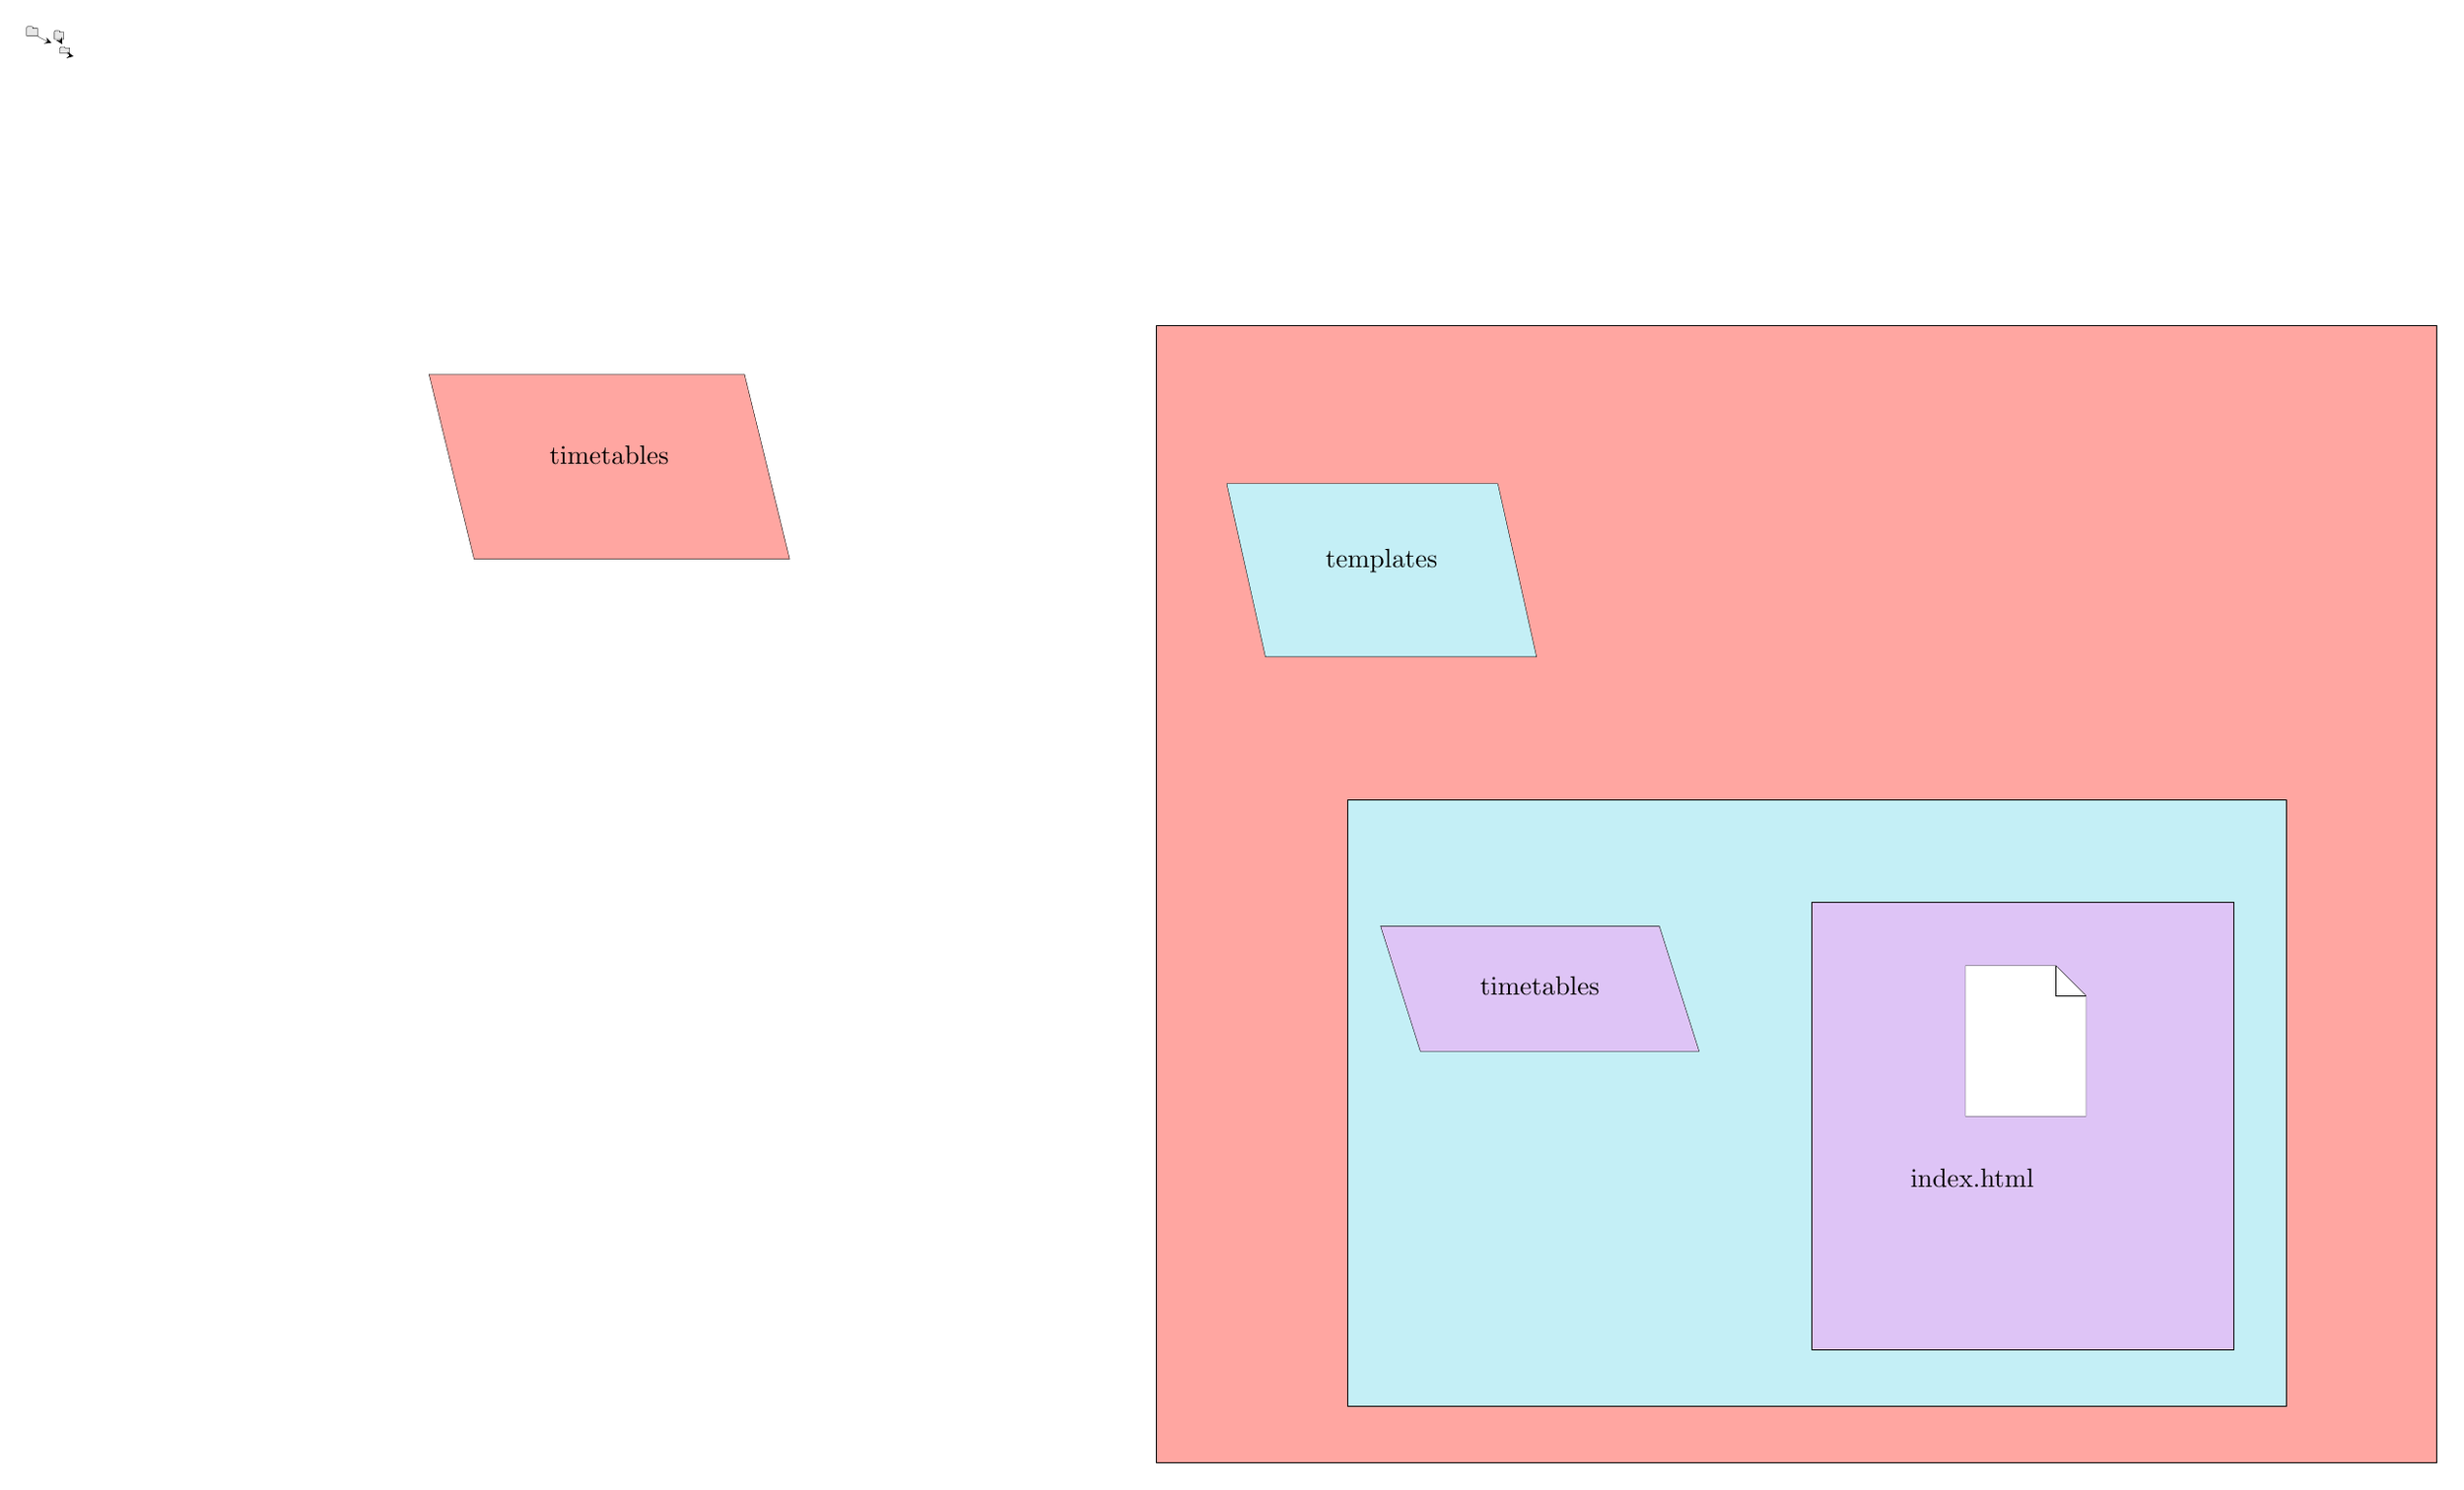
\begin{tikzpicture}
\pgftransformxscale{1.000000}
\pgftransformyscale{-1.000000}
\definecolor{dialinecolor}{rgb}{0.000000, 0.000000, 0.000000}
\pgfsetstrokecolor{dialinecolor}
\definecolor{dialinecolor}{rgb}{1.000000, 1.000000, 1.000000}
\pgfsetfillcolor{dialinecolor}
\pgfsetlinewidth{0.100000\du}
\pgfsetdash{}{0pt}
\pgfsetdash{}{0pt}
\pgfsetbuttcap
\pgfsetmiterjoin
\pgfsetlinewidth{0.100000\du}
\pgfsetbuttcap
\pgfsetmiterjoin
\pgfsetdash{}{0pt}
\definecolor{dialinecolor}{rgb}{0.901961, 0.901961, 0.901961}
\pgfsetfillcolor{dialinecolor}
\pgfpathmoveto{\pgfpoint{6.155357\du}{4.400000\du}}
\pgfpathcurveto{\pgfpoint{6.155357\du}{3.700000\du}}{\pgfpoint{6.155357\du}{3.700000\du}}{\pgfpoint{6.753572\du}{3.700000\du}}
\pgfpathcurveto{\pgfpoint{7.351786\du}{3.700000\du}}{\pgfpoint{7.351786\du}{3.700000\du}}{\pgfpoint{7.950000\du}{3.700000\du}}
\pgfpathcurveto{\pgfpoint{8.548214\du}{3.700000\du}}{\pgfpoint{8.548214\du}{3.700000\du}}{\pgfpoint{8.548214\du}{4.400000\du}}
\pgfpathcurveto{\pgfpoint{8.548214\du}{4.400000\du}}{\pgfpoint{10.342857\du}{4.400000\du}}{\pgfpoint{10.342857\du}{4.400000\du}}
\pgfpathcurveto{\pgfpoint{10.342857\du}{4.400000\du}}{\pgfpoint{10.342857\du}{7.200000\du}}{\pgfpoint{10.342857\du}{7.200000\du}}
\pgfpathcurveto{\pgfpoint{10.342857\du}{7.200000\du}}{\pgfpoint{6.155357\du}{7.200000\du}}{\pgfpoint{6.155357\du}{7.200000\du}}
\pgfpathcurveto{\pgfpoint{6.155357\du}{7.200000\du}}{\pgfpoint{6.155357\du}{5.100000\du}}{\pgfpoint{6.155357\du}{4.400000\du}}
\pgfusepath{fill}
\definecolor{dialinecolor}{rgb}{0.000000, 0.000000, 0.000000}
\pgfsetstrokecolor{dialinecolor}
\pgfpathmoveto{\pgfpoint{6.155357\du}{4.400000\du}}
\pgfpathcurveto{\pgfpoint{6.155357\du}{3.700000\du}}{\pgfpoint{6.155357\du}{3.700000\du}}{\pgfpoint{6.753572\du}{3.700000\du}}
\pgfpathcurveto{\pgfpoint{7.351786\du}{3.700000\du}}{\pgfpoint{7.351786\du}{3.700000\du}}{\pgfpoint{7.950000\du}{3.700000\du}}
\pgfpathcurveto{\pgfpoint{8.548214\du}{3.700000\du}}{\pgfpoint{8.548214\du}{3.700000\du}}{\pgfpoint{8.548214\du}{4.400000\du}}
\pgfpathcurveto{\pgfpoint{8.548214\du}{4.400000\du}}{\pgfpoint{10.342857\du}{4.400000\du}}{\pgfpoint{10.342857\du}{4.400000\du}}
\pgfpathcurveto{\pgfpoint{10.342857\du}{4.400000\du}}{\pgfpoint{10.342857\du}{7.200000\du}}{\pgfpoint{10.342857\du}{7.200000\du}}
\pgfpathcurveto{\pgfpoint{10.342857\du}{7.200000\du}}{\pgfpoint{6.155357\du}{7.200000\du}}{\pgfpoint{6.155357\du}{7.200000\du}}
\pgfpathcurveto{\pgfpoint{6.155357\du}{7.200000\du}}{\pgfpoint{6.155357\du}{5.100000\du}}{\pgfpoint{6.155357\du}{4.400000\du}}
\pgfusepath{stroke}
\pgfsetlinewidth{0.010000\du}
\pgfsetbuttcap
\pgfsetmiterjoin
\pgfsetdash{}{0pt}
\definecolor{dialinecolor}{rgb}{0.000000, 0.000000, 0.000000}
\pgfsetstrokecolor{dialinecolor}
\pgfpathmoveto{\pgfpoint{6.155357\du}{4.400000\du}}
\pgfpathcurveto{\pgfpoint{6.155357\du}{3.700000\du}}{\pgfpoint{6.155357\du}{3.700000\du}}{\pgfpoint{6.753572\du}{3.700000\du}}
\pgfpathcurveto{\pgfpoint{7.351786\du}{3.700000\du}}{\pgfpoint{7.351786\du}{3.700000\du}}{\pgfpoint{7.950000\du}{3.700000\du}}
\pgfpathcurveto{\pgfpoint{8.548214\du}{3.700000\du}}{\pgfpoint{8.548214\du}{3.700000\du}}{\pgfpoint{8.548214\du}{4.400000\du}}
\pgfpathcurveto{\pgfpoint{8.548214\du}{4.400000\du}}{\pgfpoint{10.342857\du}{4.400000\du}}{\pgfpoint{10.342857\du}{4.400000\du}}
\pgfpathcurveto{\pgfpoint{10.342857\du}{4.400000\du}}{\pgfpoint{10.342857\du}{7.200000\du}}{\pgfpoint{10.342857\du}{7.200000\du}}
\pgfpathcurveto{\pgfpoint{10.342857\du}{7.200000\du}}{\pgfpoint{6.155357\du}{7.200000\du}}{\pgfpoint{6.155357\du}{7.200000\du}}
\pgfpathcurveto{\pgfpoint{6.155357\du}{7.200000\du}}{\pgfpoint{6.155357\du}{5.100000\du}}{\pgfpoint{6.155357\du}{4.400000\du}}
\pgfusepath{stroke}
\pgfsetlinewidth{0.100000\du}
\pgfsetbuttcap
\pgfsetmiterjoin
\pgfsetdash{}{0pt}
\definecolor{dialinecolor}{rgb}{1.000000, 0.650980, 0.631373}
\pgfsetfillcolor{dialinecolor}
\fill (6.155357\du,7.200000\du)--(5.557143\du,4.750000\du)--(9.744643\du,4.750000\du)--(10.342857\du,7.200000\du)--cycle;
\definecolor{dialinecolor}{rgb}{0.000000, 0.000000, 0.000000}
\pgfsetstrokecolor{dialinecolor}
\draw (6.155357\du,7.200000\du)--(5.557143\du,4.750000\du)--(9.744643\du,4.750000\du)--(10.342857\du,7.200000\du)--cycle;
\pgfsetlinewidth{0.010000\du}
\pgfsetbuttcap
\pgfsetmiterjoin
\pgfsetdash{}{0pt}
\definecolor{dialinecolor}{rgb}{0.000000, 0.000000, 0.000000}
\pgfsetstrokecolor{dialinecolor}
\draw (6.155357\du,7.200000\du)--(5.557143\du,4.750000\du)--(9.744643\du,4.750000\du)--(10.342857\du,7.200000\du)--cycle;
% setfont left to latex
\definecolor{dialinecolor}{rgb}{0.000000, 0.000000, 0.000000}
\pgfsetstrokecolor{dialinecolor}
\node at (7.950000\du,5.825000\du){timetables};
\pgfsetlinewidth{0.100000\du}
\pgfsetdash{}{0pt}
\pgfsetdash{}{0pt}
\pgfsetmiterjoin
\definecolor{dialinecolor}{rgb}{1.000000, 0.650980, 0.631373}
\pgfsetfillcolor{dialinecolor}
\fill (15.200000\du,4.100000\du)--(15.200000\du,19.200000\du)--(32.200000\du,19.200000\du)--(32.200000\du,4.100000\du)--cycle;
\definecolor{dialinecolor}{rgb}{0.000000, 0.000000, 0.000000}
\pgfsetstrokecolor{dialinecolor}
\draw (15.200000\du,4.100000\du)--(15.200000\du,19.200000\du)--(32.200000\du,19.200000\du)--(32.200000\du,4.100000\du)--cycle;
\pgfsetlinewidth{0.100000\du}
\pgfsetdash{}{0pt}
\pgfsetdash{}{0pt}
\pgfsetbuttcap
{
\definecolor{dialinecolor}{rgb}{0.000000, 0.000000, 0.000000}
\pgfsetfillcolor{dialinecolor}
% was here!!!
\pgfsetarrowsend{stealth}
\definecolor{dialinecolor}{rgb}{0.000000, 0.000000, 0.000000}
\pgfsetstrokecolor{dialinecolor}
\pgfpathmoveto{\pgfpoint{10.169341\du}{7.248377\du}}
\pgfpatharc{121}{111}{34.149333\du and 34.149333\du}
\pgfusepath{stroke}
}
\pgfsetlinewidth{0.100000\du}
\pgfsetdash{}{0pt}
\pgfsetdash{}{0pt}
\pgfsetbuttcap
\pgfsetmiterjoin
\pgfsetlinewidth{0.100000\du}
\pgfsetbuttcap
\pgfsetmiterjoin
\pgfsetdash{}{0pt}
\definecolor{dialinecolor}{rgb}{0.901961, 0.901961, 0.901961}
\pgfsetfillcolor{dialinecolor}
\pgfpathmoveto{\pgfpoint{16.658214\du}{5.870000\du}}
\pgfpathcurveto{\pgfpoint{16.658214\du}{5.212500\du}}{\pgfpoint{16.658214\du}{5.212500\du}}{\pgfpoint{17.172143\du}{5.212500\du}}
\pgfpathcurveto{\pgfpoint{17.686072\du}{5.212500\du}}{\pgfpoint{17.686072\du}{5.212500\du}}{\pgfpoint{18.200000\du}{5.212500\du}}
\pgfpathcurveto{\pgfpoint{18.713929\du}{5.212500\du}}{\pgfpoint{18.713929\du}{5.212500\du}}{\pgfpoint{18.713929\du}{5.870000\du}}
\pgfpathcurveto{\pgfpoint{18.713929\du}{5.870000\du}}{\pgfpoint{20.255714\du}{5.870000\du}}{\pgfpoint{20.255714\du}{5.870000\du}}
\pgfpathcurveto{\pgfpoint{20.255714\du}{5.870000\du}}{\pgfpoint{20.255714\du}{8.500000\du}}{\pgfpoint{20.255714\du}{8.500000\du}}
\pgfpathcurveto{\pgfpoint{20.255714\du}{8.500000\du}}{\pgfpoint{16.658214\du}{8.500000\du}}{\pgfpoint{16.658214\du}{8.500000\du}}
\pgfpathcurveto{\pgfpoint{16.658214\du}{8.500000\du}}{\pgfpoint{16.658214\du}{6.527500\du}}{\pgfpoint{16.658214\du}{5.870000\du}}
\pgfusepath{fill}
\definecolor{dialinecolor}{rgb}{0.000000, 0.000000, 0.000000}
\pgfsetstrokecolor{dialinecolor}
\pgfpathmoveto{\pgfpoint{16.658214\du}{5.870000\du}}
\pgfpathcurveto{\pgfpoint{16.658214\du}{5.212500\du}}{\pgfpoint{16.658214\du}{5.212500\du}}{\pgfpoint{17.172143\du}{5.212500\du}}
\pgfpathcurveto{\pgfpoint{17.686072\du}{5.212500\du}}{\pgfpoint{17.686072\du}{5.212500\du}}{\pgfpoint{18.200000\du}{5.212500\du}}
\pgfpathcurveto{\pgfpoint{18.713929\du}{5.212500\du}}{\pgfpoint{18.713929\du}{5.212500\du}}{\pgfpoint{18.713929\du}{5.870000\du}}
\pgfpathcurveto{\pgfpoint{18.713929\du}{5.870000\du}}{\pgfpoint{20.255714\du}{5.870000\du}}{\pgfpoint{20.255714\du}{5.870000\du}}
\pgfpathcurveto{\pgfpoint{20.255714\du}{5.870000\du}}{\pgfpoint{20.255714\du}{8.500000\du}}{\pgfpoint{20.255714\du}{8.500000\du}}
\pgfpathcurveto{\pgfpoint{20.255714\du}{8.500000\du}}{\pgfpoint{16.658214\du}{8.500000\du}}{\pgfpoint{16.658214\du}{8.500000\du}}
\pgfpathcurveto{\pgfpoint{16.658214\du}{8.500000\du}}{\pgfpoint{16.658214\du}{6.527500\du}}{\pgfpoint{16.658214\du}{5.870000\du}}
\pgfusepath{stroke}
\pgfsetlinewidth{0.010000\du}
\pgfsetbuttcap
\pgfsetmiterjoin
\pgfsetdash{}{0pt}
\definecolor{dialinecolor}{rgb}{0.000000, 0.000000, 0.000000}
\pgfsetstrokecolor{dialinecolor}
\pgfpathmoveto{\pgfpoint{16.658214\du}{5.870000\du}}
\pgfpathcurveto{\pgfpoint{16.658214\du}{5.212500\du}}{\pgfpoint{16.658214\du}{5.212500\du}}{\pgfpoint{17.172143\du}{5.212500\du}}
\pgfpathcurveto{\pgfpoint{17.686072\du}{5.212500\du}}{\pgfpoint{17.686072\du}{5.212500\du}}{\pgfpoint{18.200000\du}{5.212500\du}}
\pgfpathcurveto{\pgfpoint{18.713929\du}{5.212500\du}}{\pgfpoint{18.713929\du}{5.212500\du}}{\pgfpoint{18.713929\du}{5.870000\du}}
\pgfpathcurveto{\pgfpoint{18.713929\du}{5.870000\du}}{\pgfpoint{20.255714\du}{5.870000\du}}{\pgfpoint{20.255714\du}{5.870000\du}}
\pgfpathcurveto{\pgfpoint{20.255714\du}{5.870000\du}}{\pgfpoint{20.255714\du}{8.500000\du}}{\pgfpoint{20.255714\du}{8.500000\du}}
\pgfpathcurveto{\pgfpoint{20.255714\du}{8.500000\du}}{\pgfpoint{16.658214\du}{8.500000\du}}{\pgfpoint{16.658214\du}{8.500000\du}}
\pgfpathcurveto{\pgfpoint{16.658214\du}{8.500000\du}}{\pgfpoint{16.658214\du}{6.527500\du}}{\pgfpoint{16.658214\du}{5.870000\du}}
\pgfusepath{stroke}
\pgfsetlinewidth{0.100000\du}
\pgfsetbuttcap
\pgfsetmiterjoin
\pgfsetdash{}{0pt}
\definecolor{dialinecolor}{rgb}{0.768627, 0.937255, 0.964706}
\pgfsetfillcolor{dialinecolor}
\fill (16.658214\du,8.500000\du)--(16.144286\du,6.198750\du)--(19.741786\du,6.198750\du)--(20.255714\du,8.500000\du)--cycle;
\definecolor{dialinecolor}{rgb}{0.000000, 0.000000, 0.000000}
\pgfsetstrokecolor{dialinecolor}
\draw (16.658214\du,8.500000\du)--(16.144286\du,6.198750\du)--(19.741786\du,6.198750\du)--(20.255714\du,8.500000\du)--cycle;
\pgfsetlinewidth{0.010000\du}
\pgfsetbuttcap
\pgfsetmiterjoin
\pgfsetdash{}{0pt}
\definecolor{dialinecolor}{rgb}{0.000000, 0.000000, 0.000000}
\pgfsetstrokecolor{dialinecolor}
\draw (16.658214\du,8.500000\du)--(16.144286\du,6.198750\du)--(19.741786\du,6.198750\du)--(20.255714\du,8.500000\du)--cycle;
% setfont left to latex
\definecolor{dialinecolor}{rgb}{0.000000, 0.000000, 0.000000}
\pgfsetstrokecolor{dialinecolor}
\node at (18.200000\du,7.220625\du){templates};
\pgfsetlinewidth{0.100000\du}
\pgfsetdash{}{0pt}
\pgfsetdash{}{0pt}
\pgfsetmiterjoin
\definecolor{dialinecolor}{rgb}{0.768627, 0.937255, 0.964706}
\pgfsetfillcolor{dialinecolor}
\fill (17.750000\du,10.400000\du)--(17.750000\du,18.450000\du)--(30.200000\du,18.450000\du)--(30.200000\du,10.400000\du)--cycle;
\definecolor{dialinecolor}{rgb}{0.000000, 0.000000, 0.000000}
\pgfsetstrokecolor{dialinecolor}
\draw (17.750000\du,10.400000\du)--(17.750000\du,18.450000\du)--(30.200000\du,18.450000\du)--(30.200000\du,10.400000\du)--cycle;
\pgfsetlinewidth{0.100000\du}
\pgfsetdash{}{0pt}
\pgfsetdash{}{0pt}
\pgfsetbuttcap
{
\definecolor{dialinecolor}{rgb}{0.000000, 0.000000, 0.000000}
\pgfsetfillcolor{dialinecolor}
% was here!!!
\pgfsetarrowsend{stealth}
\definecolor{dialinecolor}{rgb}{0.000000, 0.000000, 0.000000}
\pgfsetstrokecolor{dialinecolor}
\pgfpathmoveto{\pgfpoint{18.797055\du}{8.549536\du}}
\pgfpatharc{161}{150}{10.385761\du and 10.385761\du}
\pgfusepath{stroke}
}
\pgfsetlinewidth{0.100000\du}
\pgfsetdash{}{0pt}
\pgfsetdash{}{0pt}
\pgfsetbuttcap
\pgfsetmiterjoin
\pgfsetlinewidth{0.100000\du}
\pgfsetbuttcap
\pgfsetmiterjoin
\pgfsetdash{}{0pt}
\definecolor{dialinecolor}{rgb}{0.901961, 0.901961, 0.901961}
\pgfsetfillcolor{dialinecolor}
\pgfpathmoveto{\pgfpoint{18.714286\du}{11.837500\du}}
\pgfpathcurveto{\pgfpoint{18.714286\du}{11.362500\du}}{\pgfpoint{18.714286\du}{11.362500\du}}{\pgfpoint{19.242857\du}{11.362500\du}}
\pgfpathcurveto{\pgfpoint{19.771429\du}{11.362500\du}}{\pgfpoint{19.771429\du}{11.362500\du}}{\pgfpoint{20.300000\du}{11.362500\du}}
\pgfpathcurveto{\pgfpoint{20.828572\du}{11.362500\du}}{\pgfpoint{20.828572\du}{11.362500\du}}{\pgfpoint{20.828572\du}{11.837500\du}}
\pgfpathcurveto{\pgfpoint{20.828572\du}{11.837500\du}}{\pgfpoint{22.414286\du}{11.837500\du}}{\pgfpoint{22.414286\du}{11.837500\du}}
\pgfpathcurveto{\pgfpoint{22.414286\du}{11.837500\du}}{\pgfpoint{22.414286\du}{13.737500\du}}{\pgfpoint{22.414286\du}{13.737500\du}}
\pgfpathcurveto{\pgfpoint{22.414286\du}{13.737500\du}}{\pgfpoint{18.714286\du}{13.737500\du}}{\pgfpoint{18.714286\du}{13.737500\du}}
\pgfpathcurveto{\pgfpoint{18.714286\du}{13.737500\du}}{\pgfpoint{18.714286\du}{12.312500\du}}{\pgfpoint{18.714286\du}{11.837500\du}}
\pgfusepath{fill}
\definecolor{dialinecolor}{rgb}{0.000000, 0.000000, 0.000000}
\pgfsetstrokecolor{dialinecolor}
\pgfpathmoveto{\pgfpoint{18.714286\du}{11.837500\du}}
\pgfpathcurveto{\pgfpoint{18.714286\du}{11.362500\du}}{\pgfpoint{18.714286\du}{11.362500\du}}{\pgfpoint{19.242857\du}{11.362500\du}}
\pgfpathcurveto{\pgfpoint{19.771429\du}{11.362500\du}}{\pgfpoint{19.771429\du}{11.362500\du}}{\pgfpoint{20.300000\du}{11.362500\du}}
\pgfpathcurveto{\pgfpoint{20.828572\du}{11.362500\du}}{\pgfpoint{20.828572\du}{11.362500\du}}{\pgfpoint{20.828572\du}{11.837500\du}}
\pgfpathcurveto{\pgfpoint{20.828572\du}{11.837500\du}}{\pgfpoint{22.414286\du}{11.837500\du}}{\pgfpoint{22.414286\du}{11.837500\du}}
\pgfpathcurveto{\pgfpoint{22.414286\du}{11.837500\du}}{\pgfpoint{22.414286\du}{13.737500\du}}{\pgfpoint{22.414286\du}{13.737500\du}}
\pgfpathcurveto{\pgfpoint{22.414286\du}{13.737500\du}}{\pgfpoint{18.714286\du}{13.737500\du}}{\pgfpoint{18.714286\du}{13.737500\du}}
\pgfpathcurveto{\pgfpoint{18.714286\du}{13.737500\du}}{\pgfpoint{18.714286\du}{12.312500\du}}{\pgfpoint{18.714286\du}{11.837500\du}}
\pgfusepath{stroke}
\pgfsetlinewidth{0.010000\du}
\pgfsetbuttcap
\pgfsetmiterjoin
\pgfsetdash{}{0pt}
\definecolor{dialinecolor}{rgb}{0.000000, 0.000000, 0.000000}
\pgfsetstrokecolor{dialinecolor}
\pgfpathmoveto{\pgfpoint{18.714286\du}{11.837500\du}}
\pgfpathcurveto{\pgfpoint{18.714286\du}{11.362500\du}}{\pgfpoint{18.714286\du}{11.362500\du}}{\pgfpoint{19.242857\du}{11.362500\du}}
\pgfpathcurveto{\pgfpoint{19.771429\du}{11.362500\du}}{\pgfpoint{19.771429\du}{11.362500\du}}{\pgfpoint{20.300000\du}{11.362500\du}}
\pgfpathcurveto{\pgfpoint{20.828572\du}{11.362500\du}}{\pgfpoint{20.828572\du}{11.362500\du}}{\pgfpoint{20.828572\du}{11.837500\du}}
\pgfpathcurveto{\pgfpoint{20.828572\du}{11.837500\du}}{\pgfpoint{22.414286\du}{11.837500\du}}{\pgfpoint{22.414286\du}{11.837500\du}}
\pgfpathcurveto{\pgfpoint{22.414286\du}{11.837500\du}}{\pgfpoint{22.414286\du}{13.737500\du}}{\pgfpoint{22.414286\du}{13.737500\du}}
\pgfpathcurveto{\pgfpoint{22.414286\du}{13.737500\du}}{\pgfpoint{18.714286\du}{13.737500\du}}{\pgfpoint{18.714286\du}{13.737500\du}}
\pgfpathcurveto{\pgfpoint{18.714286\du}{13.737500\du}}{\pgfpoint{18.714286\du}{12.312500\du}}{\pgfpoint{18.714286\du}{11.837500\du}}
\pgfusepath{stroke}
\pgfsetlinewidth{0.100000\du}
\pgfsetbuttcap
\pgfsetmiterjoin
\pgfsetdash{}{0pt}
\definecolor{dialinecolor}{rgb}{0.870588, 0.768627, 0.964706}
\pgfsetfillcolor{dialinecolor}
\fill (18.714286\du,13.737500\du)--(18.185714\du,12.075000\du)--(21.885714\du,12.075000\du)--(22.414286\du,13.737500\du)--cycle;
\definecolor{dialinecolor}{rgb}{0.000000, 0.000000, 0.000000}
\pgfsetstrokecolor{dialinecolor}
\draw (18.714286\du,13.737500\du)--(18.185714\du,12.075000\du)--(21.885714\du,12.075000\du)--(22.414286\du,13.737500\du)--cycle;
\pgfsetlinewidth{0.010000\du}
\pgfsetbuttcap
\pgfsetmiterjoin
\pgfsetdash{}{0pt}
\definecolor{dialinecolor}{rgb}{0.000000, 0.000000, 0.000000}
\pgfsetstrokecolor{dialinecolor}
\draw (18.714286\du,13.737500\du)--(18.185714\du,12.075000\du)--(21.885714\du,12.075000\du)--(22.414286\du,13.737500\du)--cycle;
% setfont left to latex
\definecolor{dialinecolor}{rgb}{0.000000, 0.000000, 0.000000}
\pgfsetstrokecolor{dialinecolor}
\node at (20.300000\du,12.868750\du){timetables};
\pgfsetlinewidth{0.100000\du}
\pgfsetdash{}{0pt}
\pgfsetdash{}{0pt}
\pgfsetmiterjoin
\definecolor{dialinecolor}{rgb}{0.870588, 0.768627, 0.964706}
\pgfsetfillcolor{dialinecolor}
\fill (23.900000\du,11.750000\du)--(23.900000\du,17.700000\du)--(29.500000\du,17.700000\du)--(29.500000\du,11.750000\du)--cycle;
\definecolor{dialinecolor}{rgb}{0.000000, 0.000000, 0.000000}
\pgfsetstrokecolor{dialinecolor}
\draw (23.900000\du,11.750000\du)--(23.900000\du,17.700000\du)--(29.500000\du,17.700000\du)--(29.500000\du,11.750000\du)--cycle;
\pgfsetlinewidth{0.100000\du}
\pgfsetdash{}{0pt}
\pgfsetdash{}{0pt}
\pgfsetbuttcap
{
\definecolor{dialinecolor}{rgb}{0.000000, 0.000000, 0.000000}
\pgfsetfillcolor{dialinecolor}
% was here!!!
\pgfsetarrowsend{stealth}
\definecolor{dialinecolor}{rgb}{0.000000, 0.000000, 0.000000}
\pgfsetstrokecolor{dialinecolor}
\pgfpathmoveto{\pgfpoint{21.405180\du}{13.787280\du}}
\pgfpatharc{129}{101}{5.560462\du and 5.560462\du}
\pgfusepath{stroke}
}
\pgfsetlinewidth{0.100000\du}
\pgfsetdash{}{0pt}
\pgfsetdash{}{0pt}
\pgfsetbuttcap
\pgfsetmiterjoin
\pgfsetlinewidth{0.100000\du}
\pgfsetbuttcap
\pgfsetmiterjoin
\pgfsetdash{}{0pt}
\definecolor{dialinecolor}{rgb}{1.000000, 1.000000, 1.000000}
\pgfsetfillcolor{dialinecolor}
\fill (25.950000\du,12.600000\du)--(27.150000\du,12.600000\du)--(27.550000\du,13.000000\du)--(27.550000\du,14.600000\du)--(25.950000\du,14.600000\du)--cycle;
\definecolor{dialinecolor}{rgb}{0.000000, 0.000000, 0.000000}
\pgfsetstrokecolor{dialinecolor}
\draw (25.950000\du,12.600000\du)--(27.150000\du,12.600000\du)--(27.550000\du,13.000000\du)--(27.550000\du,14.600000\du)--(25.950000\du,14.600000\du)--cycle;
\pgfsetbuttcap
\pgfsetmiterjoin
\pgfsetdash{}{0pt}
\definecolor{dialinecolor}{rgb}{0.000000, 0.000000, 0.000000}
\pgfsetstrokecolor{dialinecolor}
\draw (27.150000\du,12.600000\du)--(27.150000\du,13.000000\du)--(27.550000\du,13.000000\du)--(27.550000\du,13.000000\du);
% setfont left to latex
\definecolor{dialinecolor}{rgb}{0.000000, 0.000000, 0.000000}
\pgfsetstrokecolor{dialinecolor}
\node[anchor=west] at (25.100000\du,15.425000\du){index.html};
\end{tikzpicture}
}
\caption{Estructura de directorios de las plantillas de \texttt{Django}}
\label{djangotemplates}
\end{figure}

Las plantillas podrían colocarse directamente dentro del directorio \texttt{templates}, pero esto no es una buena práctica. ¿Por qué no? Si tenemos varias aplicaciones en nuestro proyecto y dos de ellas tienen un template con el mismo nombre, \texttt{Django} puede equivocarse de template y seleccionar uno incorrecto. Esto ocurre porque \texttt{Django} escoge el primer template que tenga el nombre deseado. Por eso, una buena forma de diferenciar ambos templates es colocarlos dentro de una carpeta que se llame igual que la aplicación, para hacer que ambos templates estén en \textit{namespaces} diferentes.

\subsubsection{¿Cómo son las plantillas de \texttt{Django}?} 
Una plantilla es simplemente un archivo de texto que puede generar archivos en cualquier tipo de formato (HTML, XML, CSV...). Una plantilla contiene \textbf{\textit{variables}}, que se reemplazan por sus respectivos valores cuando se procesa la plantilla, y \textbf{\textit{etiquetas}}, que controlan la lógica de la plantilla.

Las variables se definen entre dos llaves: \texttt{\{\{ variable \}\}}. Cuando el sistema de plantillas se encuentra con una variable, la evalúa y reemplaza con el resultado de dicha evaluación. Es importante destacar que no puede utilizarse el símbolo ``.'' en los nombres de las variables. Sí que se puede usar el símbolo ``\_''. El punto (``.'') se utliza para acceder a los atributos de una variable 

Por otro lado, las etiquetas se definen entre una llave y un símbolo de porcentaje: \texttt{\{\% etiqueta \%\}}. Pueden controlar el flujo de la plantilla a través de bucles y condiciones, entre otras cosas.

Ahora que ya sabemos cómo funcionan de forma muy básica las plantillas de \texttt{Django}, vamos a pasar a explicar las plantillas realizadas para el proyecto.

\subsubsection{La plantilla \texttt{index.html}}
\begin{figure}
\centering
\includegraphics[width=\textwidth]{img/pantalla_inicial_final}
\caption{Resultado final de la pantalla inicial}
\label{pantallainicialfinal}
\end{figure}

En la \hyperref[pantallainicialfinal]{Figura \ref*{pantallainicialfinal}} vemos el resultado final de la pantalla de inicio. Es un simple formulario con tres campos, los parámetros necesarios para generar un horario: número de días, número de horas por día y el cuatrimestre. ¿Cómo se genera esta página usando las plantillas? En este caso, he definido un formulario normal con HTML pero teniendo en cuenta los siguientes detalles:

\begin{enumerate}[$\bullet$]
  \item A la hora de definir la acción del formulario (es decir, a qué URL se va a llamar cuando se presione el botón de \textit{submit}), he usado una etiqueta para que \texttt{Django} escriba la URL correspondiente, en lugar de escribirla yo misma.

  \mint{html}|<form action="" method="post">|

  \item Cuando definimos un campo en el formulario, debemos tener claro que ese nombre es el que vamos a usar en la vista en la que procesemos el formulario. Por ejemplo, en el caso del número de días, lo he definido en el formulario de la siguiente forma:

  \mint{html}|<label for="days">Number of days</label>|

  Y a la hora de procesarlo en la vista, lo he hecho de la siguiente forma:

  \mint{python}|days = int(request.POST['days'])|

  Como se ve, el mismo nombre que se le asigna en el HTML es el que se tiene que usar después para consultar su valor.

  \item Para hacer la interfaz más usable, he añadido al formulario una validación de la entrada \cite{validatorform}. Para ello, he usado las etiquetas HTML \texttt{type}, \texttt{min} y \texttt{max} para especificar el tipo de dato (número), el valor mínimo que puede tener y el máximo:

  \begin{minted}[breaklines, breakafter=d]{html}
  <input type="number" max="5" min="4" class="form-control" name="days" placeholder="Number of days of the timetable">  
  \end{minted}

  Así, si el usuario intenta introducir ``cinco'' días a la semana, el campo erróneo del formulario se pondrá en rojo indicando que el dato introducido es erróneo, tal y como se ve en la \hyperref[validationerrornumber]{Figura \ref*{validationerrornumber}}.

  \begin{figure}
    \centering
    \includegraphics[width=\textwidth]{img/validationerrornumber}
    \caption{Error al intentar introducir el número de días de forma errónea}
    \label{validationerrornumber}
  \end{figure}

  Además, si tratamos de introducir un número demasiado alto de días el formulario también se quejará, tal y como se aprecia en la \hyperref[validationerrormax]{Figura \ref*{validationerrormax}}, porque en una semana hay, como mucho, cinco días. 

  \begin{figure}
    \centering
    \includegraphics[width=\textwidth]{img/validationerrormax}
    \caption{Error al intentar introducir un número demasiado alto de días}
    \label{validationerrormax}
  \end{figure}

  Es importante destacar que \textbf{esto no es una medida de seguridad, sino de usabilidad}. Es decir, a pesar de tener esta validación de la entrada en el \textit{frontend}, es obligatorio validar la entrada en el \textit{backend}. ¿Por qué? Porque desde el editor de HTML de cualquier navegador es posible eliminar la validación, tal y como se ve en la \hyperref[seguridad0]{Figura \ref*{seguridad0}}. Si esto ocurriese, el servidor tendría que detectarlo y dar una excepción como la que se ve en la \hyperref[seguridadback]{Figura \ref*{seguridadback}}. Por tanto, esta validación en el formulario sólo se hace para ayudar al usuario a saber qué datos tiene que introducir pero no es, ni de lejos, una medida de seguridad.

  \begin{displayquote}
    ``En el \textit{frontend}, no hay seguridad.''
  \end{displayquote}

  \begin{figure}
    \centering
    \includegraphics[width=\textwidth]{img/seguridad0}
    \caption{Desde el editor HTML de cualquier navegador es posible cambiar el campo \texttt{type="number"} a \texttt{type="text"} y saltar así la validación}
    \label{seguridad0}
  \end{figure}

  \begin{figure}
    \centering
    \includegraphics[width=\textwidth]{img/seguridadback}
    \caption{Excepción en el backend cuando se introduce un número de días no válido}
    \label{seguridadback}
  \end{figure}
\end{enumerate}

\subsubsection{La plantilla \texttt{showdata.html}}
\begin{figure}
  \centering
  \includegraphics[width=\textwidth]{img/pantalla_horario_final}
  \caption{Resultado final de la pantalla para mostrar los horarios}
  \label{finalhorarios}
\end{figure}

En la \hyperref[finalhorarios]{Figura \ref*{finalhorarios}} vemos el resultado final de la pantalla para mostrar horarios. En este caso, la pantalla tiene tres partes:

\begin{enumerate}[---]
  \item La más importante de todas, es una tabla en la cual se muestra el horario del grupo seleccionado.
  \item Para seleccionar grupo, hay un \textit{dropdown} que permite seleccionar el grupo deseado.
  \item Y, por último, un botón para imprimir el horario en PDF.
\end{enumerate}

Como dije antes, la tabla se envía a la plantilla en forma de diccionario JSON. Dicho diccionario JSON tiene como claves las distintas horas del día (``$8:30\;-\;9:30$'', ``$9:30\;-\;10:30$''$\ldots$) y como valores, la lista de asignaturas y aulas para cada día. Es importante tener clara esta estructura para poder comprender mejor cómo se genera la tabla. Para generar la tabla, itero usando una etiqueta \texttt{for} por todo el diccionario:

\mint{django}||

Dentro de cada hora de la semana, es importante distinguir si es de teoría o de prácticas. Ya que una hora de prácticas ocupa una única celda mientras que una de teoría ocupa tantas celdas como subgrupos de prácticas haya. Esto es así debido a que en HTML, al igual que en \LaTeX, no es posible dividir una celda pero sí es posible agrupar $n$ celdas. Para ello, he usado el atributo HTML \texttt{colspan}:

\begin{minted}{django}
<tr>
  
    
      
        <td>{{ s }}</td>
      
    
      <td colspan="{{ request.session.numsubgroups }}">{{ column.subject }}</td>
    
  
</tr>
\end{minted}

Otro detalle importante es el de las filas: al igual que en el PDF de horarios que hay actualmente, la clase en la que se imparte una asignatura se coloca justo debajo de su nombre. Para hacer esto en HTML, he tenido que hacer que la celda que indica las horas ocupe dos filas: una fila para indicar el nombre de la asignatura y otra, para indicar la clase en la que se imparte. Para ello, he usado el atributo HTML \texttt{rowspan}:

\mint{html}|<th scope="row" rowspan="2"> {{ hour }}</th>|

Finalmente, los días de la semana son parte de la cabecera de la tabla. Al igual que con las celdas de teoría, ocuparán tantas celdas como subgrupos de prácticas haya:

\begin{minted}{html}
<thead class="thead-inverse">
  <tr>
    <th>Hour</th>
    <th colspan="{{ request.session.numsubgroups }}">Monday</th>
    <th colspan="{{ request.session.numsubgroups }}">Tuesday</th>
    <th colspan="{{ request.session.numsubgroups }}">Wednesday</th>
    <th colspan="{{ request.session.numsubgroups }}">Thursday</th>
    <th colspan="{{ request.session.numsubgroups }}">Friday</th>
  </tr>
</thead>
\end{minted}

Para generar el \textit{dropdown}, lo único que he hecho ha sido iterar una lista que contiene los nombres de todos los grupos. \texttt{Django} automáticamente genera un enlace por cada elemento de la lista.

\begin{minted}[breaklines, breakafter=d]{html}
<div class="dropdown-menu" aria-labelledby="dropdownMenuButton">
  
    <a class="dropdown-item" href="">{{ group }}</a>
  
</div>
\end{minted}

En la \hyperref[dropdowngrupos]{Figura \ref*{dropdowngrupos}} se ve cómo queda al final este elemento. Es muy importante destacar cómo con tres líneas de código, \texttt{Django} es capaz de generar dinámicamente toda la lista de enlaces.

\begin{figure}
  \centering
  \includegraphics[width=\textwidth]{img/horario_horario_grupos}
  \caption{Pantalla para mostrar los horarios, con el \textit{dropdown} de grupos desplegado}
  \label{dropdowngrupos}
\end{figure}

Por último, para generar el botón de imprimir en PDF, lo único que he tenido que hacer ha sido añadir un enlace con la URL que definimos para generar los PDFs:

\begin{minted}[breaklines, breakafter=d]{html}
<div class="col" style="text-align: right">
  <a href=""><button type="button" class="btn btn-primary">Generate PDF</button></a>
</div>
\end{minted}

\subsubsection{Usando el framework \textit{Bootstrap} para definir el estilo de la página}
Para hacer que la página tenga un estilo más moderno y actual, he utilizado \textbf{Bootstrap} (\url{https://getbootstrap.com/}). \textit{Bootstrap} permite construir sitios web \textit{responsive} y con un toque moderno de forma rápida y sencilla. Tiene predefinidos un montón de estilos para diferentes elementos HTML como formularios, tablas, botones, barras de navegación...

Me decidí a usar \textit{Bootstrap} para poder centrarme en los aspectos más importantes del sistema, seguridad y usabilidad, y no estar perdiendo el tiempo con el CSS. Yo soy partidaria de usar herramientas ya hechas, en lugar de perder el tiempo haciendo una herramienta desde 0. Entiendo que haya sistemas en los que sea necesario hacer un desarrollo completo, ya que no disponen de conexión a internet para descargar dependencias externas pero, en este caso, no se daba esa condición. 

Para usar \textit{Bootstrap}, lo único que hay que hacer es importar el framework en la cabecera del HTML y usar en los elementos HTML las clases CSS definidas por \textit{Bootstrap}, utilizando la etiqueta \texttt{class}. De esta forma, en un breve espacio de tiempo hemos conseguido lo que nos podría llevar perfectamente una semana entera.
